\documentclass[output=paper, chinesefont]{langscibook}
\ChapterDOI{10.5281/zenodo.15006621}
\author{Ho Wang Matthew Sung\orcid{}\affiliation{Leiden University} and Jelena Prokić\orcid{}\affiliation{Leiden University} and Yiya Chen\orcid{}\affiliation{Leiden University}}
\title[Applying tonal distance metrics to a large dialectal dataset]{Applying the state-of-the-art tonal distance metrics to a large dialectal dataset}
\abstract{From \posscitet{Seguy1971, Seguy1973} early dialectometric studies to the application of Levenshtein distance in dialectometry (e.g. \citealt{Heeringa2004}) nowadays, the calculation of phonetic distances between dialects has largely been focused on segments. Despite the fact that tonal languages make up to 70\% of the languages in the world \citep[1]{Yip2002}, tones are still largely neglected or simplified in comparative dialectological studies. In the current literature, there are very limited attempts to quantify tone distances between dialects. Furthermore, these methods were mostly designed for perceptual studies and most importantly, they were tested with a rather small dialect dataset (20 or fewer dialects, e.g. \citealt{YangCastro2008}, \citealt{Tang2009}). When the method is not tested on a larger dataset, it is unclear how many tones a particular representation used in a distance calculation method can differentiate, and if it can be applied across different languages. An ideal method to calculate tone distances should be able to differentiate all possible tones in a given set of dialects, and not be bounded to specific datasets only. 

In this chapter, we have compared four ways in calculating tone distances using data from Yue and Pinghua dialects, two Sinitic branches from the Sinto-Tibetan language family which are spoken in Guangdong and Guangxi provinces in Southern China. They are chosen for this study because Yue and Pinghua provide a huge amount of data, both segmental and tonal. Furthermore, their tonal inventories consist of a wide range of tone types, differing in pitch, contour, shape, and duration. Our results show that some methods are more suitable for dialectometry, though they still require further improvements before we can apply them to investigate tonal variation.}

\IfFileExists{../localcommands.tex}{
  \addbibresource{../localbibliography.bib}
  \usepackage{tabularx,multicol}
%\usepackage{multirow}
\usepackage{subcaption}
\usepackage{url}
\urlstyle{same}

\usepackage{datetime}
\usepackage{enumitem}
\usepackage{langsci-optional}
\usepackage{langsci-lgr}
\usepackage{langsci-branding}

\usepackage{longtable}
\usepackage{xltabular}
\usepackage[linguistics, edges]{forest}
\usepackage{pgfplots}
\pgfplotsset{compat=1.18}
\usetikzlibrary{patterns, tikzmark}
\usepackage{pgfplotstable}
\usepgfplotslibrary{colorbrewer}
\usepackage{listings}
\lstset{basicstyle=\ttfamily,keywordstyle=\normalfont,language=,breaklines=true}

\usepackage{siunitx}
\sisetup{group-digits=none, detect-all=true}

\usepackage{langsci-gb4e}

  \makeatletter
\let\thetitle\@title
\let\theauthor\@author
\makeatother

% Use this Chinese font shipped with TeX Live instead of Source Han, because
% it is more portable/leightweight. Install the "fandol" package from CTAN to
% automatically get this font.
\newfontfamily{\ChineseFandolSong}{FandolSong-Regular.otf}
 
  %% hyphenation points for line breaks
%% Normally, automatic hyphenation in LaTeX is very good
%% If a word is mis-hyphenated, add it to this file
%%
%% add information to TeX file before \begin{document} with:
%% %% hyphenation points for line breaks
%% Normally, automatic hyphenation in LaTeX is very good
%% If a word is mis-hyphenated, add it to this file
%%
%% add information to TeX file before \begin{document} with:
%% %% hyphenation points for line breaks
%% Normally, automatic hyphenation in LaTeX is very good
%% If a word is mis-hyphenated, add it to this file
%%
%% add information to TeX file before \begin{document} with:
%% \include{localhyphenation}
\hyphenation{
    a-na-ly-sis
    ap-proach-es
    ar-che-o-log-i-cal
    Ar-khan-gelsk
    be-schrei-ben
    Buch-holtz
    Che-lya-binsk
    con-so-nant
    dia-lect
    dia-lect-ology
    Di-a-lekt-for-schung
    Dia-lekt-for-schung
    East-pha-lian
    För-der-ung
    Ge-mein-schaft-lich-keits-ent-wür-fe
    his-tor-i-cal
    Hok-kai-do
    ja-pa-nese
    Ja-pa-nese
    Ka-go-shi-ma
    Ka-li-nin-grad
    Knja-zev
    Ma-kro-be-reich
    Ma-lay-sia
    mor-pho-log-i-cal
    Mos-cow
    Nef-te-yu-gansk
    non-mobile
    nu-cle-ar
    ös-ter-rei-chi-sche
    par-a-digm
    per-zep-ti-ons-lin-gu-is-ti-sche
    plu-ri-zen-tri-schen
    quick-ly
    Reich
    Sax-on
    Schrö-der
    sear-ching
    ste-reo-type
    strength-en-ing
    strong-est
    Stutt-gart
    su-pra-seg-men-tal
    teach-er
    to-po-gra-phy
    To-ron-to
    tra-di-tion-al
    ul-ti-mate-ly
    Um-gangs-spra-che
    Volks-kun-de
    vor-zu-stel-len
    wheth-er
    Wie-sing-er
    with-in
    Wort-at-las
}

\hyphenation{
    a-na-ly-sis
    ap-proach-es
    ar-che-o-log-i-cal
    Ar-khan-gelsk
    be-schrei-ben
    Buch-holtz
    Che-lya-binsk
    con-so-nant
    dia-lect
    dia-lect-ology
    Di-a-lekt-for-schung
    Dia-lekt-for-schung
    East-pha-lian
    För-der-ung
    Ge-mein-schaft-lich-keits-ent-wür-fe
    his-tor-i-cal
    Hok-kai-do
    ja-pa-nese
    Ja-pa-nese
    Ka-go-shi-ma
    Ka-li-nin-grad
    Knja-zev
    Ma-kro-be-reich
    Ma-lay-sia
    mor-pho-log-i-cal
    Mos-cow
    Nef-te-yu-gansk
    non-mobile
    nu-cle-ar
    ös-ter-rei-chi-sche
    par-a-digm
    per-zep-ti-ons-lin-gu-is-ti-sche
    plu-ri-zen-tri-schen
    quick-ly
    Reich
    Sax-on
    Schrö-der
    sear-ching
    ste-reo-type
    strength-en-ing
    strong-est
    Stutt-gart
    su-pra-seg-men-tal
    teach-er
    to-po-gra-phy
    To-ron-to
    tra-di-tion-al
    ul-ti-mate-ly
    Um-gangs-spra-che
    Volks-kun-de
    vor-zu-stel-len
    wheth-er
    Wie-sing-er
    with-in
    Wort-at-las
}

\hyphenation{
    a-na-ly-sis
    ap-proach-es
    ar-che-o-log-i-cal
    Ar-khan-gelsk
    be-schrei-ben
    Buch-holtz
    Che-lya-binsk
    con-so-nant
    dia-lect
    dia-lect-ology
    Di-a-lekt-for-schung
    Dia-lekt-for-schung
    East-pha-lian
    För-der-ung
    Ge-mein-schaft-lich-keits-ent-wür-fe
    his-tor-i-cal
    Hok-kai-do
    ja-pa-nese
    Ja-pa-nese
    Ka-go-shi-ma
    Ka-li-nin-grad
    Knja-zev
    Ma-kro-be-reich
    Ma-lay-sia
    mor-pho-log-i-cal
    Mos-cow
    Nef-te-yu-gansk
    non-mobile
    nu-cle-ar
    ös-ter-rei-chi-sche
    par-a-digm
    per-zep-ti-ons-lin-gu-is-ti-sche
    plu-ri-zen-tri-schen
    quick-ly
    Reich
    Sax-on
    Schrö-der
    sear-ching
    ste-reo-type
    strength-en-ing
    strong-est
    Stutt-gart
    su-pra-seg-men-tal
    teach-er
    to-po-gra-phy
    To-ron-to
    tra-di-tion-al
    ul-ti-mate-ly
    Um-gangs-spra-che
    Volks-kun-de
    vor-zu-stel-len
    wheth-er
    Wie-sing-er
    with-in
    Wort-at-las
}
 
  \togglepaper[1]%%chapternumber
}{}


\begin{document}



\graphicspath{{figures/sung}}
\maketitle 
%ATTENTION: Diacritics on the following phonetic characters might have been lost during conversion: {'ɛ'}
\label{chap:sung}

\section{Introduction}
\label{sec:sung:1}

Traditional dialectology (also known as dialect geography, \citealt{ChambersTrudgill1998}: 14) originated in Europe, pioneered in Germany and France, has primarily been centering around phonetics and lexicon, and syntax has entered the scene more recently. The study of phonetic variation has been heavily focused on segments, and not tones, despite the fact that 60-70\% of the world’s languages also include lexical tones. This focus is not surprising, however, since European languages mostly do not use pitch to differentiate word meaning. Although the traditional methodology of dialect geography spread to different corners of the world, the application of computational mapping, later computational processing of dialectal data, has mostly been developed and applied to European languages, such as Dutch \citep{Heeringa2004} and French \citep{Goebl1984}. For the same reason, these computational methods do not concern tonal variation, and whether these methods are suitable for the tonal data is a current issue yet to be solved.

In Chinese dialectology, for example, there are numerous studies on dialects spoken in China (e.g. \citegen{Chao1928} survey on Wu dialects, Grootaers’s work on Shanxi \citep{Grootaers2003}, \citegen{Zhan2002} \textit{Introduction to Yue dialects in Guangdong}), and it has a century-long tradition, but most studies on tonal variation are descriptive. This means that studies usually report the tonal inventory of a dialect after a fieldwork investigation, and/or tones are analyzed in terms of how they correspond to historical tone categories (from the Middle Chinese period, based on the rhyme dictionary descriptions). An example of such studies is \citet{Zhan2002}. Although there is a huge amount of dialect data available for Chinese (in the form of IPA transcriptions, including tones), currently we are still at the exploration stage in finding a methodology which allows dialectologists to measure tone distances for the purpose of dialect classification.  The lack of analytic tools is not only a problem for dialectologists working with Chinese, but for dialectologists, as well as linguists, around the world. While most of the world’s languages are tonal, we do not have proper methods which would allow us to investigate dialectal variation of tones, the most important aspect of tonal languages by which they differ from the non-tonal languages.

The structure of this paper is as follows: \sectref{sec:sung:1} briefly sketches what tonal languages are and their relative isolation in dialectometry. \sectref{sec:sung:2} gives an overview of the current approaches to quantifying phonetic tone distances, with more focus on the replicable methods. \sectref{sec:sung:3} introduces the Yue and Pinghua dialects, which serve as the case study for this paper, and their sources of data, as well as a sketch of the methodology used in comparing different methods in calculating tone distances introduced in \sectref{sec:sung:2}. \sectref{sec:sung:4} presents the results of the comparisons as well as their interpretations and lastly, \sectref{sec:sung:5} and \sectref{sec:sung:6} offer the discussion and conclusions respectively.

\section{Tonal languages and dialectometry}
\label{sec:sung:2}
According to \citet[229]{Hyman2006}, tones can be defined as the use of “pitch… [in] the lexical realization of at least some morphemes”. It has been estimated that around 60--70\% of the languages in the world are tonal \citep[1]{Yip2002}. Some relatively well-studied tonal languages include Cantonese, Mandarin and Yoruba.

The main types of tone contour are Level, Falling, Rising, as well as complex tones Concave (Falling-Rising) and Convex (Rising-Falling) tones. A level tone is a tone with a contour that is kept flat throughout the whole tone production.\footnote{In reality, some of the Level tones also have a slight falling or rising F0 trajectory, but this paper focuses on impressionistic transcription data, which does not always capture such fine trajectories.}  A rising tone is when the pitch of the offset is higher than the onset, whereas a falling tone is the opposite. Concave and convex tones are the combinations of Rising and Falling tones. Languages and dialects may have more than one tone of the same contour. For example, Cantonese has three level tones, two rising tones and one falling tone. It has been found that across 737 Sinitic varieties (including over 500 Mandarin dialects), Falling tone is the most common tone (1125 tokens), closely followed by Level tones (1086 tokens). Rising (790 tokens) and Concave (352 tokens) tones are less common and Convex (80 tokens) tones are the least common \citep{Cheng1973}.

There are very limited attempts to quantify tone distances between dialects, like \citet{YangCastro2008} and \citet{Tang2009}. Furthermore, these methods were mostly designed for perceptual studies and most importantly, they were tested on a rather small dialect dataset (20 or fewer dialects). When the tone representation used in a particular method is not tested on a larger dataset, it is unclear how many tones it can differentiate, and if it can be applied across different languages. An ideal method to calculate tone distances should be able to differentiate all possible tones in a given set of dialects, and not be bounded to specific datasets only. 

In this study we rely on the Yue and Pinghua dialects to explore the possibility of measuring tone distances between dialects using computational methods. We made this choice because Yue and Pinghua provide a huge amount of data, especially on tones. The tonal inventories of Yue and Pinghua dialects consist of a wide range of tone types, differing in pitch, contour, shape, and duration. A wide range of tone types is necessary for the development of a way to measure tone distances, since this method is aimed to be applicable to all tonal languages in the world, provided the suitable transcriptions are given. It should be noted that the transcriptions of tones for Yue and Pinghua are impressionistic, meaning that the distances cannot capture fine trajectories and it may be subjected to transcribers’ differences. However, this is understandable, since a lot of the Yue and Pinghua data, as well as other Chinese varieties and possibly other tonal language dialect surveys, were collected before portable recorders were available for data collection. 

\section{Previous approaches to measuring tone distances}
\label{sec:sung:3}
\subsection{Background}
\label{sec:sung:3.1}

\begin{sloppypar}
Most studies in dialectology (descended from the dialect geographical tradition) have been conducted on Indo-European languages and other non-tonal languages (including pitch-accent languages like Japanese). Therefore, there is a lack of dialect geographical studies that involve tones. For tonal languages such as Sinitic languages, most research is rather descriptive, i.e., listing the tonal inventory of a dialect or showing diachronic correspondences with historical tone categories, as in \citegen{Zhan2002} \textit{Introduction to the Yue dialects in Guangdong}, for example.
\end{sloppypar}

The same problem can be found in dialectometry, the subdiscipline of dialectology which applies quantitative and computational methods to study dialects. From Séguy's (\citeyear{Seguy1971,Seguy1973}) enterprise of aggregating linguistic features to the application of Levenshtein distance (e.g. \citealt{Heeringa2004}), segments have always been the focus of the studies in dialectometry. Up to date, there are no large-scale dialectometric studies on tones; the highest number of dialects involved are no more than 20 (see \citealt{YangCastro2008}, \citealt{Tang2009}). In some dialectometric studies, tones were neglected (e.g. \citealt{WichmannRan2019}), others used a rather simplified method (e.g. \citealt{Stanford2012}). In addition, there are studies on the correlation between phonetic distance and the perception of tones (e.g. \citealt{YangCastro2008}), which do not focus on the application of these measures on dialect classification.

At least for Sinitic languages, there is an abundance of data available for tones (transcriptions), but not enough is known on the incorporation of these data with segments. Tones in Chinese dialectology are most commonly written in \citegen{Chao1930} notation, known as the \textit{tone letters}. The tone letters is a transcription system which consists of 5 digits, \textit{1}, \textit{2}, \textit{3}, \textit{4}, \textit{5}, and they represent different (possible) contour levels in a tone. \textit{1} represents the lowest contour level and \textit{5} represents the highest, while the rests sit in between. When combined (as two digits or three digits) together, they can indicate a change in the contour, which represent the shape of the tone. For example, \textsuperscript{53} is a falling tone, whereas \textsuperscript{213} is a dipping tone (a falling contour followed by a rising contour).

In the following subsections we will discuss four previously proposed methods for measuring tone distances and point some drawbacks (see \sectref{sec:sung:3} for the data).

\subsection{Onset-Contour-Offset}
\label{sec:sung:3.2}
Onset-Contour-Offset (OCO hereafter) is a representation of tones proposed by \citet{YangCastro2008}. This representation gives a more phonetic representation of tones, instead of an abstract one, as its purpose is to approximate multiple cues of tones in the distance measure in order to generate a more accurate prediction for intelligibility between dialects. 

OCO involves a transformation of the tone letters (5-level transcription, \citealt{Chao1930}) into a representation which consists of three components: \textit{Onset}, \textit{Contour} and \textit{Offset}, each represented with one character, except for Contour, which can have up to two characters. Onset and Offset are the starting and ending contour levels of the tone, and the Contour is the shape of the tone. For the contour levels, the original 5-level transcription is converted into three categories, which are \textit{H(igh)}, \textit{M(id)} and \textit{L(ow)}. H represents levels 4 and 5, M represents 3 and L represents 1 and 2. For contours, the basic shapes include \textit{R(ising)}, \textit{F(alling)}, \textit{L(evel)}, and the complex tones are represented by the combination of the basic shapes, hence it has up to two characters.\footnote{The complex tones are additions to Yang and Castro’s original proposal, as the original article did not account for these types of tone, but they are present in our dataset.} Examples of the Contour representations can be found in \tabref{tab:sung:1}.

\begin{table}
\begin{tabular}{llc}
\lsptoprule
{Representation} & {Contour} & {Examples}\\\midrule
L & Level & 11, 33\\
R & Rising & 12, 35\\
F & Falling & 31, 52\\
RF & Convex & 131, 253\\
FR & Concave & 213, 424\\
\lspbottomrule
\end{tabular}
\caption{Contours in OCO representation with examples}
\label{tab:sung:1}
\end{table}

As an example, the OCO representation of 221 would be LLFL, and for 24, it would be LRH. To calculate tone distances, \citet{YangCastro2008} applied the Levenshtein distance algorithm on the OCO representation. This is illustrated in \tabref{tab:sung:2}. 

When two tones with different lengths are compared (length of three and four, like in \tabref{tab:sung:2}), the Onset (Slot 1) and Offset (Slot 4) are always aligned together. In this example, we can find two substitutions and one deletion out of four alignment slots. This yields a (3 / 4 =) 0.75 difference between the tone pair.


\begin{table}
\begin{tabular}{cccccc}
\lsptoprule
{Slot 1} & {Slot 2} & {Slot 3} & {Slot 4} & {Operations} & {Distance}\\\midrule
 L & L & F & L & {}- & {}-\\
 L & R & F & L & Substitution of L > R & 1\\
 L & R & \_ & L & Deletion of F & 1\\
 L & R &  & H & Substitution of L > H & 1\\
\multicolumn{5}{c}{\raggedleft Sum} & 3\\
\lspbottomrule
\end{tabular}
\caption{Calculation of Levenshtein Distance between 221 and 24 in OCO representation}
\label{tab:sung:2}
\end{table}

Last but not least, the aggregated distance is calculated by summing the tone distances of the tone pairs and dividing the sum by the number of words compared in pairwise comparison between two dialects. This is done for any dialect pair in the dataset.

OCO has shown high correlation with mutual intelligibility for both Zhuang and Bai in \citegen{YangCastro2008} study. \citegen{DoLai2021} results basically agree with Yang and Castro. However, \citet[122--125]{Tang2009} found that OCO fails to yield a classification which can differentiate Mandarin from other Sinitic languages. Based on this result, \citet[125]{Tang2009} argued that this representation does not “provide a handle on dialect affinity”.

It should be mentioned that in \citet{YangCastro2008}, a related representation, Onset-Contour, correlates significantly higher than OCO with intelligibility as a predictor for Zhuang. However, because this representation can differentiate even fewer tones than OCO (see \sectref{sec:sung:4}), in this paper we focus on the OCO representation.

\subsection{Tone-to-string}
\label{sec:sung:3.3}
The tone-to-string method applies the Levenshtein distance algorithm directly on \citegen{Chao1930} tone letters. The differences in the digits are not accounted in this method, i.e. a substitution from 2 to 1 costs the same distance as from 4 to 1. In addition, when a two-digit tone is compared with a three-digit tone, the first digit of the two-digit tone aligns with the second digit of the three-digit tone\footnote{This alignment is based on \citet{Tang2009}.}, as shown in the example below. Note that in this approach short tones are not distinguished from the other tones in the dataset.

In the example in \tabref{tab:sung:3}, we illustrate how tones 325 and 15 are aligned and the distance between them is calculated using Levenshtein algorithm. In this example, one substitution and deletion are required to convert 325 to 15, which yields distance of (2 / 3 =) 0.67 between two tones.


\begin{table}
\begin{tabular}{ccccc}
\lsptoprule
{Slot 1} & {Slot 2} & {Slot 3} & {Operations} & {Distance}\\\midrule
3 & 2 & 5 & {}- & {}-\\
\_ & 2 & 5 & Deletion of 3 & 1\\
& 1 & 5 & Substitution of 2 > 1 & 1\\
\multicolumn{4}{l}{Sum} & 2\\
\lspbottomrule
\end{tabular}
\caption{Calculation of Levenshtein Distance between 325 and 15 with tone-to-string method}
\label{tab:sung:3}
\end{table}

The aggregated distance is again calculated as the sum of the tone distances of the word pairs, divided by the number of words compared in pairwise comparison between two varieties. Thus, the aggregated distance is calculated for any pair of varieties in the dataset.

\citet{YangCastro2008} has found that applying Levenshtein distance directly on \citegen{Chao1930} tone letters has a lower correlation to mutual intelligibility than OCO. \citegen{Tang2009} evaluation also shows that this method yields quite a high number of misclassifications when compared to the traditional classification (separating Mandarin from other Sinitic languages).

\subsection{Binary comparison}
\label{sec:sung:3.4}
\citet[53]{Cheng1997} proposed to calculate the similarities between dialects by measuring the ratio of shared items to all the items (segments and tones) that are occurring in both varieties in a pairwise comparison. The shared and non-shared items are indicated in binary form, i.e. with \textit{1} (present) and \textit{0} (absent) in the data matrix. This is similar to \citegen{Goebl1984} \textit{Relative Identity Value}, but the data matrix is comprised using the bag-of-words approach (based on the sound inventory of all dialects in the data). \citet[105–106]{Tang2009} has found that this method yields a number of misclassifications when compared to the traditional taxonomy (Mandarin vs. other Sinitic languages). In addition, \citet[114--115]{Tang2009} weighted the tone inventories by lexical frequency (out of 764 items in the database). This method yields one misclassification more than the binary inventory comparison. Another related approach by \citet[88-89]{Cheng1991} includes Middle Chinese sound categories (as indicated by the ancient rhyme dictionaries \textit{Guangyun}\footnote{In Chinese dialectology, \textit{Guangyun}, a rhyme dictionary which represents the phonology of Middle Chinese, is often used as a proto-system for modern Chinese dialects \citep[85-86]{YouChinDial}.}) in the data matrix, in addition to adding lexical weighting and comparing tone inventories, using more than 2700 words. The compared elements are not simply the synchronic sound segments in the inventories, but reflexes of certain Middle Chinese sound categories. For example, instead of stating Dialect A has 79 tokens of [pʰ], Dialect A now has 40 tokens of [pʰ ] as a reflex of *pʰ  and and 39 tokens of [pʰ ] as a reflex of *b. \citegen[131--132]{Tang2009} evaluation shows that the result from Cheng’s method highly resembles the traditional classification. Due to lack of proto-Yue reconstructions that we could use to annotate our data, the above method cannot be applied to our dataset. Therefore, we use the binary comparison approach. 

Comparing the tonal inventory between dialects might be too simplistic, since dialects could share the same tonal inventory (with the same phonetic tone values), but the lexical distribution \citep[78]{Wells1982} of the tones could be different. For example, the Taishan and Kaiping dialects are members of the Siyi dialects which have an identical tonal inventory, with 5 tonemes which are phonetically the same (\citealt{ZhanCheung1990}: 85–87). However, not all lexical items share the same tones. In \tabref{tab:sung:4}, we have listed three examples where each item has a different tone in each dialect.

\begin{table}
\begin{tabular}{lll}
\lsptoprule
Item & Taishan & Kaiping\\\midrule
First syllable of ‘lychee’ {\cn{荔}} & lai\textsuperscript{31}                    & lai\textsuperscript{21}\\
‘inner’ {\cn{内}}  & \textsuperscript{n}dui\textsuperscript{31} & lui\textsuperscript{22}\\
‘caldron’                  {\cn{釜}} & fu\textsuperscript{21}                     & fu\textsuperscript{55}\\
\lspbottomrule
\end{tabular}
\caption{Examples of lexical distribution differences in tones of two Siyi dialects}
\label{tab:sung:4}
\end{table}

%\todo{sign for `inner' 内 doesn't show properly} 
\begin{sloppypar}
In order to account for the lexical distribution differences between dialects, the binary comparison has been modified from the inventory level (comparing differences in the tonemic inventory only) to the lexical level (comparing tone differences in word pairs). Instead of comparing the proportion of elements (tones) shared, the tone distance for each lexical item is calculated by identifying whether the tone is identical (distance = 0) or not (distance = 1). An overall aggregate distance for each dialect pair is then calculated.
\end{sloppypar}

The binary method is a harsh measure which implies that there is no difference in the distance between similar and very different tones, i.e. 11 vs. 22 and 11 vs. 523 are equally distant.

\subsection{Gandour-Harshman-Tang tone distance}
\label{sec:sung:3.5}
Unlike the previous methods in \sectref{sec:sung:3.2}--\sectref{sec:sung:3.4}, the Gandour-Harshman-Tang tone distance is based on the perceptual experiment of tone distances published in \citet{GandourHarshman1978}. Their stimuli included a range of tones, which differ in contour, pitch and duration, and they asked listeners to rate their distances. Based on the perceived distances of the listeners (Thai, Yoruba and English), five dimensions have been extracted and interpreted as \textit{Average Height}, \textit{Direction} (Rising, Level, Falling), \textit{Length}, \textit{Extreme End Point} and \textit{Slope}. These dimensions are underlying ‘cues’ which can explain the variance found in the perceptual tone distance matrix and have been implemented as multivalued features by \citet[125--126]{Tang2009} as a way to measure objective tone distances. This is the tone distance measure which accounts for perception, unlike other methods, which have been criticized as “very crude and unrealistic”, since any substitution or changes in the pitch and contour have equal importance \citep[125]{Tang2009}. However, a method as sophisticated as this still gave “highly unsatisfactory results” according to \citegen[127]{Tang2009} evaluation method, since it also cannot differentiate Mandarin from other Sinitic languages, just like OCO.

Based on the contour of the tone, a feature value is assigned for each cue under the criteria listed in \tabref{tab:sung:5} to represent a tone, following Tang’s (2009: 125) implementation. It should be noted that in Tang’s dissertation, only the last two digits of the tone are taken into account for Direction and Slope, which means that complex tones and their counterparts without their onset element will share the same values for these two cues. 


\begin{table}
\begin{tabular}{llrr}
\lsptoprule
      &            & Feature & Maximal\\
{Cue} & {Features} & value & difference\\\midrule
Average Height & Lower than 2.5 & 1 & 4\\
               & Between 2.5 and 3.5 & 3 & \\
               & Higher than 3.5 & 5 & \\\addlinespace
Direction\footnote{last two digits} & Falling & 0 & 2\\
                            & No change/ one digit tone & 1 & \\
                            & Rising & 2 & \\\addlinespace
Duration & 1-digit (or short 2-digit) tone & 1 & 2\\
         & 2-digit (or short 3-digit) tone & 2 & \\
         & 3-digit tone & 3 & \\\addlinespace
Slope\footnote{last two digits} & Difference smaller than 3 & 0 & 1\\
                        & Difference bigger than 3 & 1 & \\\addlinespace
Extreme endpoint\footnote{final digit} & Ends with 2, 3 or 4 & 0 & 1\\
                               & Ends with 1 or 5 & 1 & \\
\lspbottomrule
\end{tabular}
\caption{Cues and their relative feature values in GH-T}
\label{tab:sung:5}
\end{table}

It should also be noted that we made a slight modification to \citegen{Tang2009} implementation. For Direction, instead of assigning the values \textit{0}, \textit{1}, \textit{2} to Level, Falling, and Rising, respectively, we have made Level as the middle value (i.e.~\textit{1}). This change can make the distances between the directions more continuous (Rising-Level-Falling forming a continuum), rather than being arbitrary categorical values. Furthermore, since this method is \citegen{Tang2009} implementation of the perceptual dimensions found by \citet{GandourHarshman1978}, this method will be addressed as the GH-T hereafter, which stands for Gandour-Harshman-Tang.

Here is an example how tone distance is calculated with GH-T, which is also illustrated in \tabref{tab:sung:6}. The maximum difference two tones can have is 10, based on sum of the maximal difference each cue can have ($4+2+2+1+1$). Take 551 and 12\# as an example (\# indicates a shorter duration of the tone, often found in checked syllables), their feature specifications of these tones are listed in \tabref{tab:sung:6}. After deducting the absolute difference of each feature value and sum the differences, this value is the distance between the tone pair. 551 and 12\# is one of the possible pairs of tones with the greatest distance in \citegen{Chao1930} transcription system, since it yields the maximum difference score this tone representation can produce.


\begin{table}
\begin{tabular}{lrrrrrr}
\lsptoprule
              &          &             &            &         &  Extreme    & \\
{Tone string} & {Height} & {Direction} & {Duration} & {Slope} & {end point} & {Total}\\\midrule
551 & 5 & 0 & 3 & 1 & 1 & \\
12\# & 1 & 2 & 1 & 0 & 0 & \\
Difference & 4 & 2 & 2 & 1 & 1 & 10\\
\lspbottomrule
\end{tabular}
\caption{Example of tone distance calculation using GH-T}
\label{tab:sung:6}
\end{table}

For the computation of GH-T, the Manhattan distance has been used. Manhattan distance in this context is the sum of absolute differences of the values for all the cues shown in \tabref{tab:sung:5} (maximum distance is 10). In addition, all the differences are divided by 10 so that the range of differences are kept between 0 and 1, just like the other metrics in the previous subsections. Again, the overall aggregated difference is calculated between all dialect pairs in the data.

\subsection{Interim summary}
\label{sec:sung:3.6}
The state-of-the-art methods in measuring tone distances range from a strict binary approach to a metric which deals with of multi-valued features (GH-T). It is important to compare these methods systematically in order to explore the applicability of these methods to a larger dialect dataset in the classification context. As we have previously mentioned, these methods have only been applied to datasets with 20 or fewer dialects. We would like to know which method(s) are more linguistically coherent and suitable for dialect classification and identify possible improvements, so that they can be applied to various tonal languages in the world.

\section{Data and methodology}
\label{sec:sung:4}
\subsection{Data}
\label{sec:sung:4.1}
The data of this study focuses on the dialects within the Yue-Pinghua-speaking area. Yue and Pinghua are two sub-branches of the Sinitic branch of the Sino-Tibetan language family, which are spoken in Southern China and the diaspora communities in North America, the UK, Malaysia etc. \citep{Wu2012Yue}.

\subsubsection{Yue and Pinghua}
\label{sec:sung:4.1.1}
Yue and Pinghua are mainly spoken in Southern China, namely in the Guangdong and Guangxi provinces \citep{CASS2012}. Their geographical distribution is shown in \figref{fig:sung:1}\footnote{All the maps in this paper are produced with \textit{QGIS} (QGIS development team 2022).} (based on the \textit{Language Atlas of China 1\textsuperscript{st}} \textit{Edition}, Li and Wurm1987)\footnote{The first edition is used because the maps provide a more precise delimitation of the Yue and Pinghua areas than the second edition, since it is based on political boundaries instead of linguistic boundaries.}.

  
\begin{figure}[t]
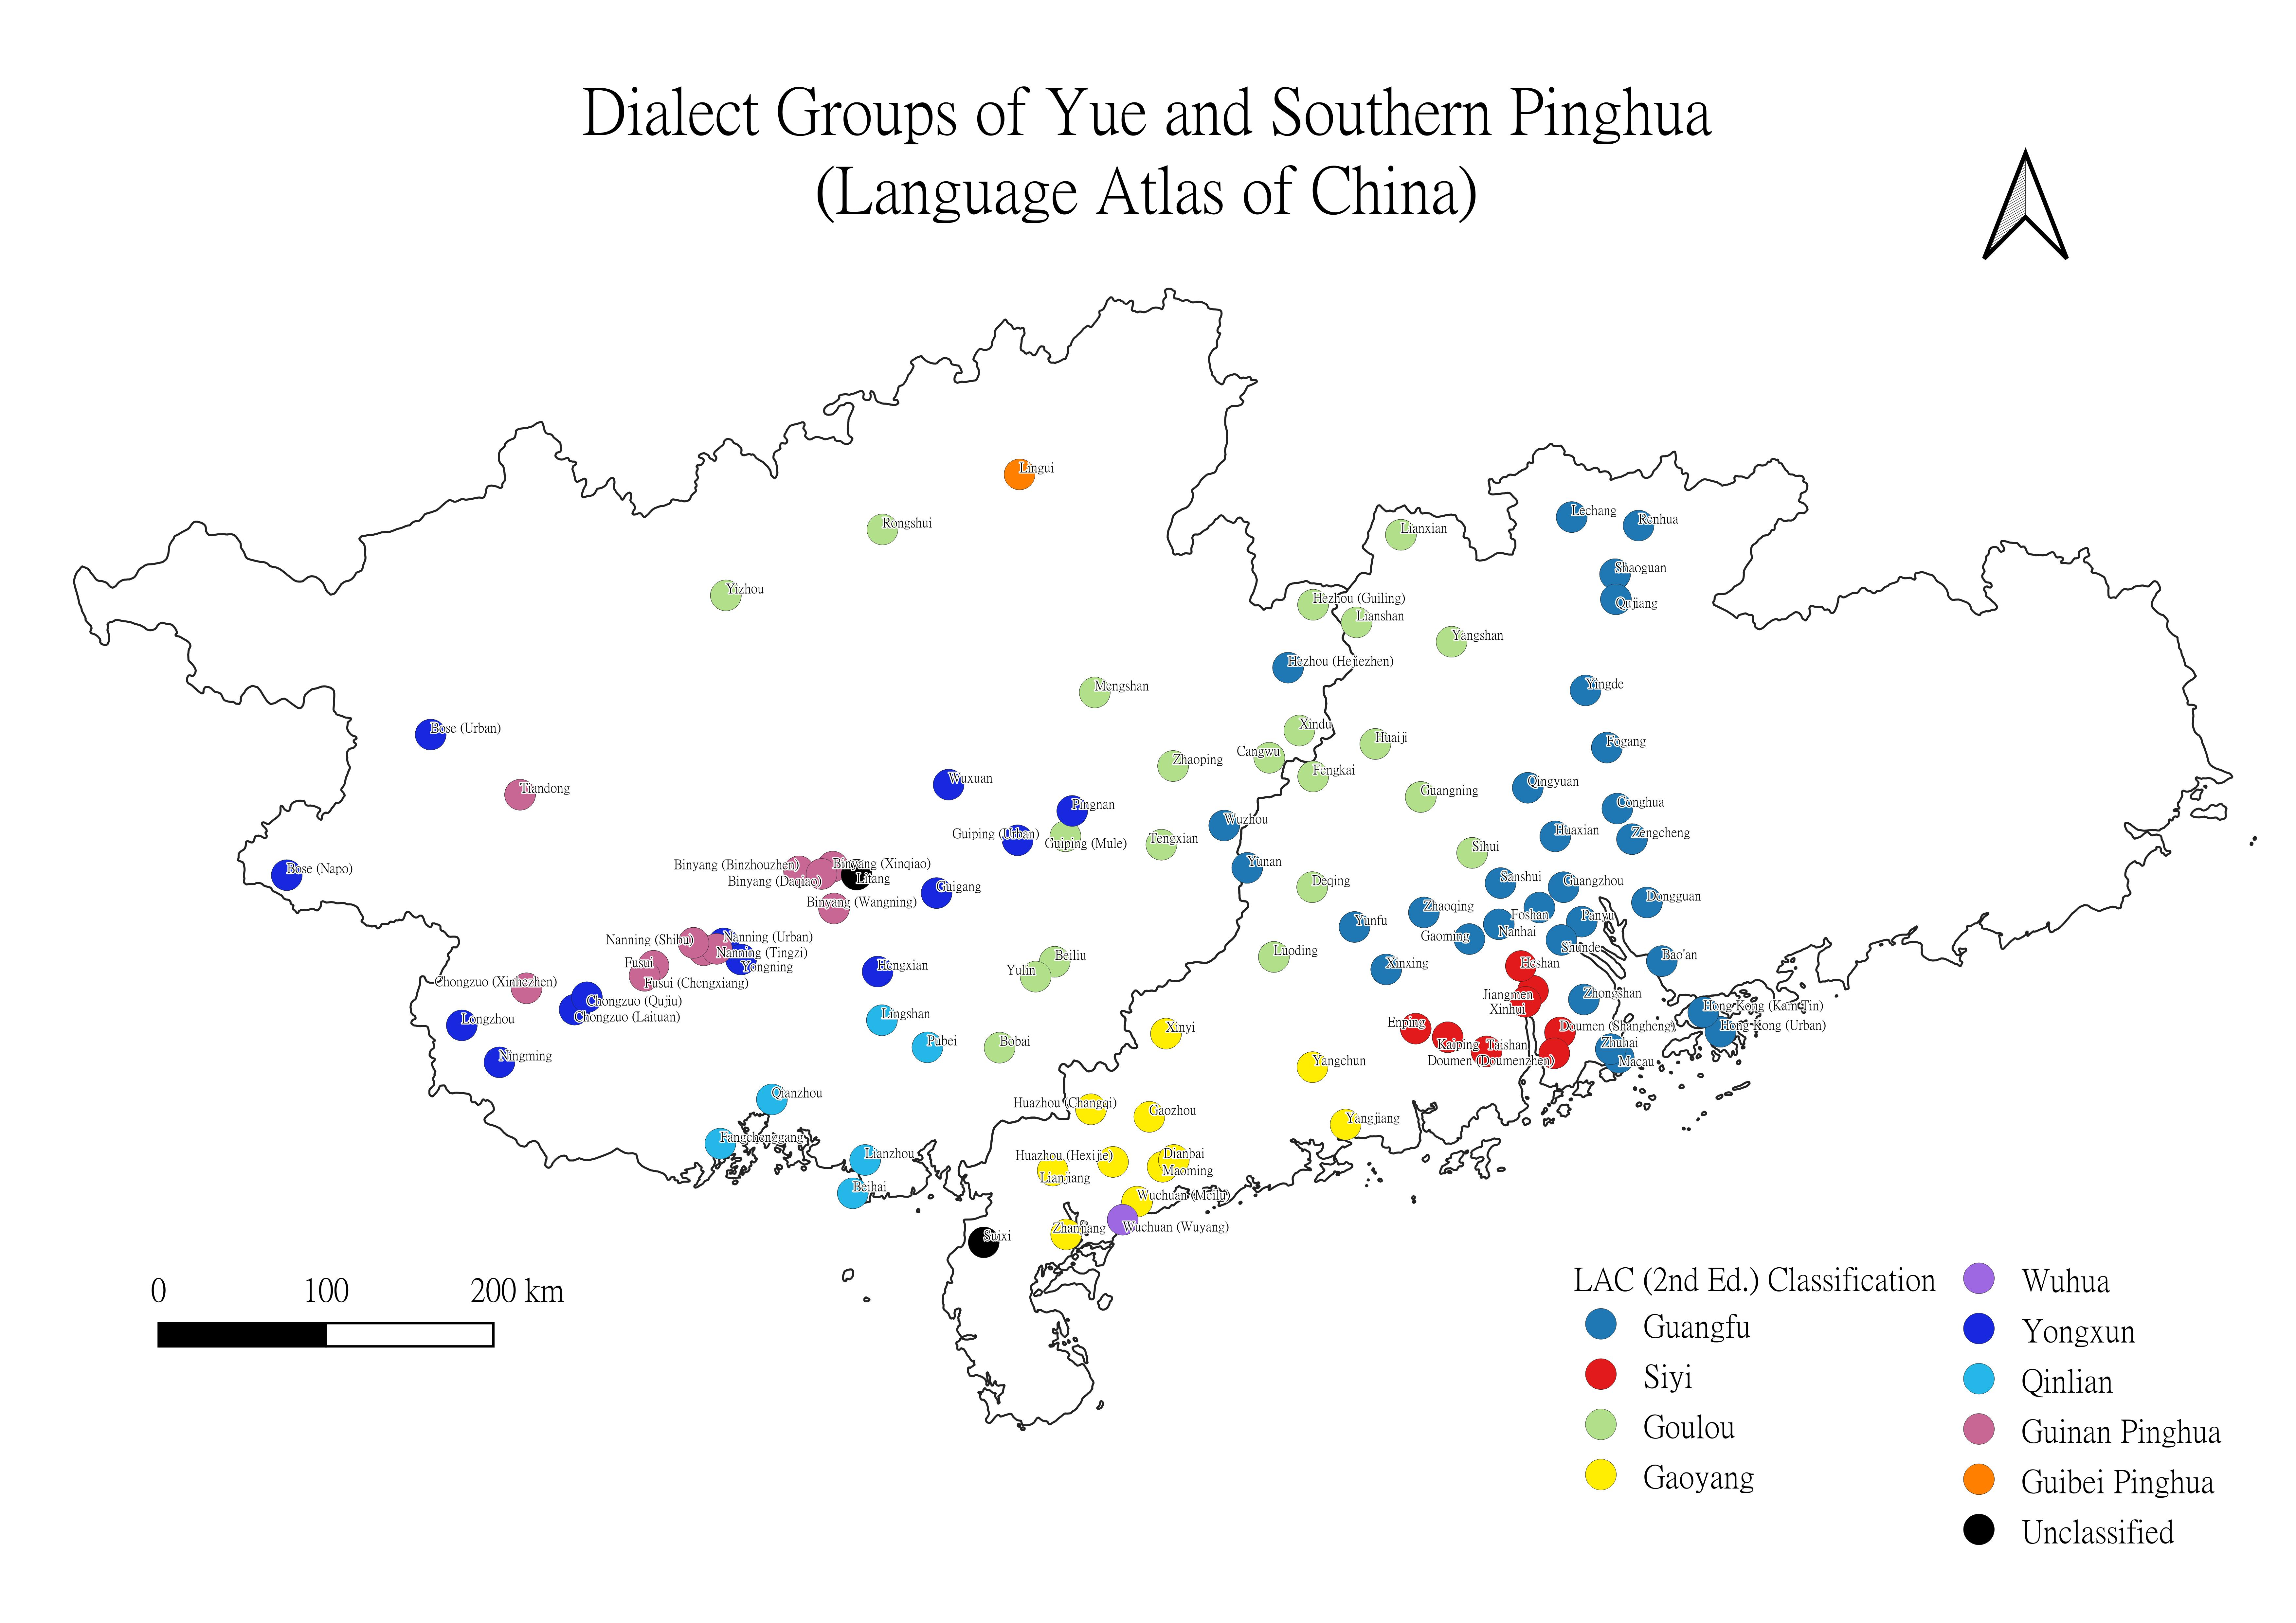
\includegraphics[width=\textwidth]{20240810 grafiken sung neu/Map 1_LAC_classification_ver4_labelled.jpeg}
 \caption{Dialect areas of Yue and Pinghua in Guangdong and Guangxi provinces (based on the Language Atlas of China 1st Edition)}
\label{fig:sung:1}
\end{figure}

Traditionally, Yue has seven dialect groups, whereas Pinghua has two major dialect groups (Northern vs. Southern). There have been several attempts in classifying the dialects within Yue. \citet{YueHashimoto1988} performed the most extensive comparison over a number of Yue dialects, with over 100 features. However, her study suffered from the lack of data in certain regions, leaving her classification incomplete. Other classifications were either focused on one area (e.g. \citealt{Zhan2002} for the Guangdong province only) or unknown criteria were used (e.g. \citealt{Zhan1981}, \citealt{Yuan2001}). The classification from the \textit{Language Atlas of China} (\textit{LAC} hereafter, 2nd Edition, \citealt{CASS2012}) covers the whole Yue-speaking region, and it stated clearly which criteria were used in the classification. A potential problem with the LAC classification is that very few features were used, and the motivation behind the choice of features has not been explained. However, since it is the only existing complete classification of Yue, it remains the representative of the traditional classification of Yue.

The status of Pinghua as a major branch of Sinitic languages has been controversial ever since its first proposal in the 1980s. Scholars have been arguing whether Pinghua belongs to Yue or not, and there have been proponents for both sides of the arguments. A group of scholars represented by \citet{LiangZhang1999}, \citet{Wei1996}, \citet{Li2000} cited in \citet{Tan2012} focused more on the differences (of features) between Pinghua and Yue, and argued that Pinghua should be independent from Yue. The opponents represented by \citet{Wu2001}, \citet{Tan2000} and \citet{Liang1997}, cited in \citet{Tan2012} examined a bunch of features and they mostly argued that a sub-branch of Pinghua, Guinan (Southern) Pinghua, is actually very similar to Yue, therefore it should be grouped under Yue. \citet{Liang1997} made an even more radical claim that the whole Pinghua branch should be merged with Yue after examining seven features.

One of the reasons why the status of Pinghua is controversial is that each scholar focused on a different set of features, some on the differences (e.g.  the reflex of Middle Chinese *kʰ{}- is often a [kʰ{}-] in Pinghua, but [h-] in Yue, \citet{Li2000}: 36), while others on the similarities (e.g. the retention of codas -p, -t, -k, \citet{Wu2001}: 137). 

\subsubsection{Segmental dialectometric classification of Yue and Pinghua}
\label{sec:sung:4.1.2}
Our preliminary dialectometric result on the segmental variation (using classic Levenshtein distance) of Yue and Pinghua somewhat resembles the opponents of the Yue-Pinghua dichotomy, that Northern Pinghua is very different from the rest of the Yue and Southern Pinghua dialects (see \figref{fig:sung:2}). 

   
\begin{figure}
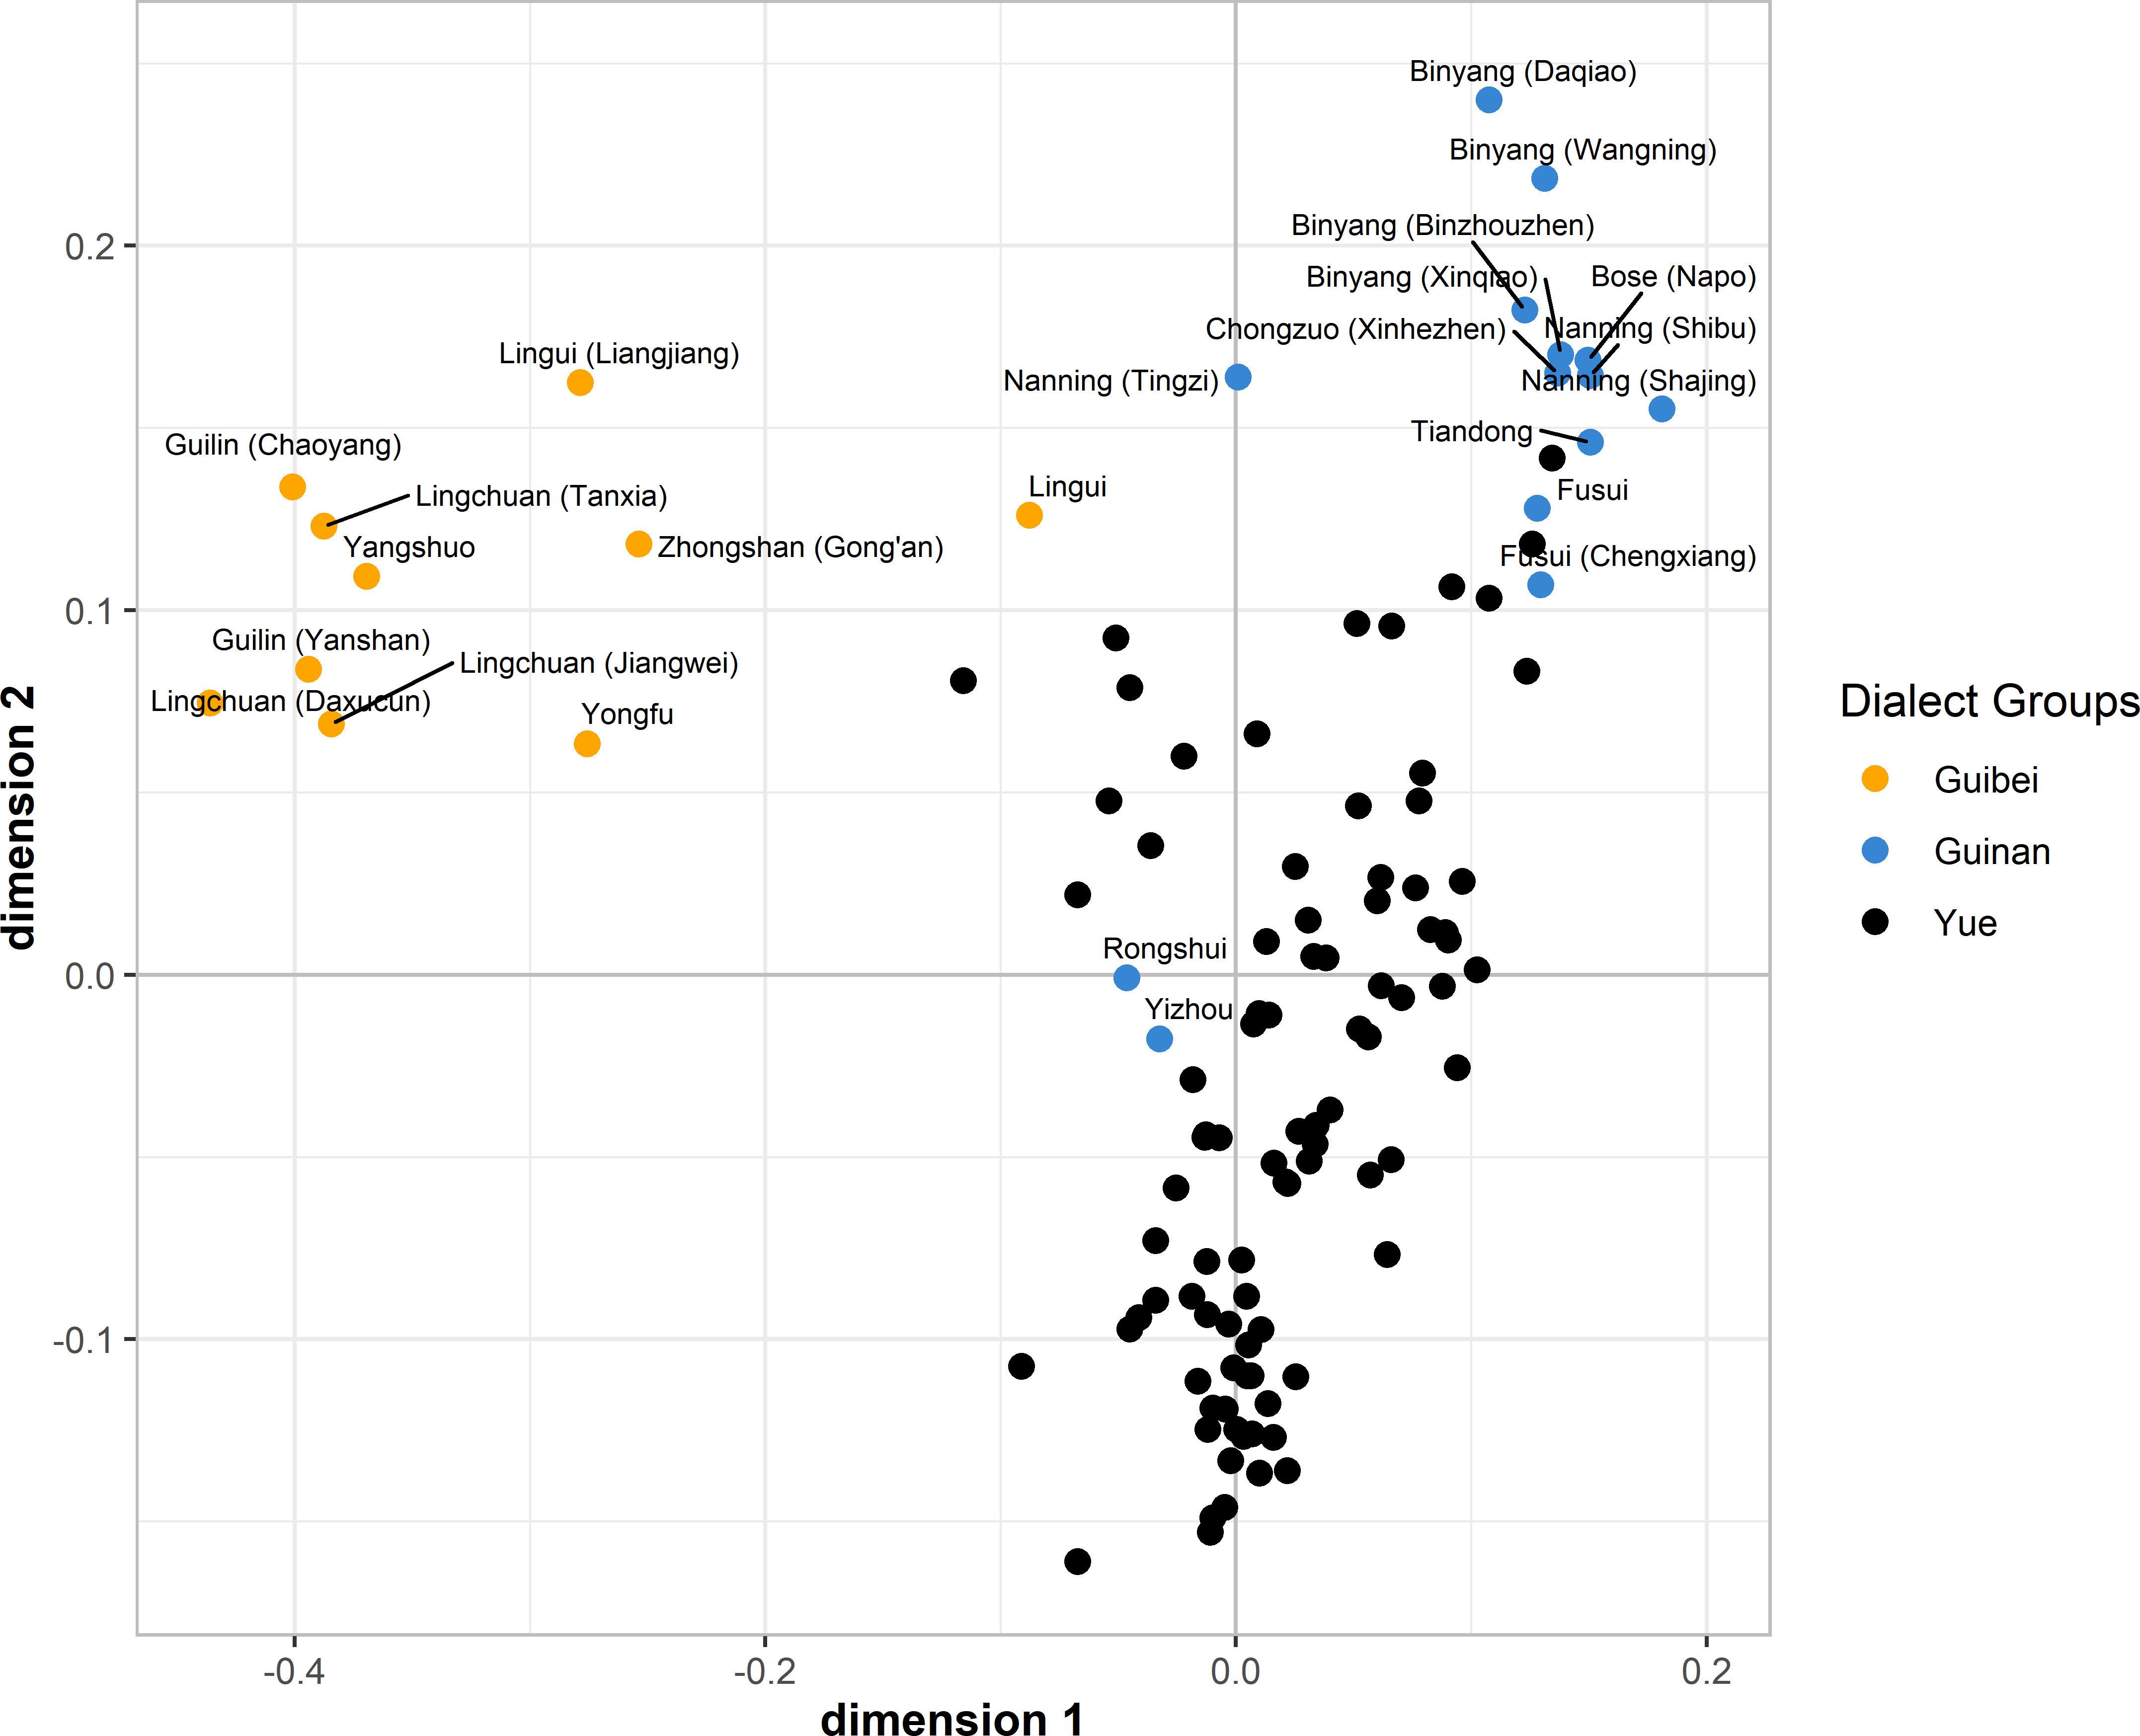
\includegraphics[width=\textwidth]{sung-img002.png}
\caption{MDS plots of 113 Yue and Pinghua dialects according to LAC, r\textsuperscript{2} = 0.59}
\label{fig:sung:2}
\end{figure}

\figref{fig:sung:2} is a multidimensional scaling plot which reduces dimensions and approximates the distances calculated between all dialects in a 2D plot. The axes, labelled as dimension 1 and 2 represent underlying patterns which explains the greatest amount of variance found in the aggregated dialect distances. We can see that most of the orange dots (traditionally classified as Northern Pinghua) are located on the left (with high negative values in the first dimension). There is one exception, i.e. the Lingui dialect, which is located much closer to 0 in dimension 1, and also towards the rest of the dialects. Furthermore, there seems to be no continuum between the Northern Pinghua dialects and the rest of the dialects, which suggests abrupt boundaries between Northern Pinghua and the Yue continuum (in black). 
This result resembles the traditional analysis.
To gain an understanding of how well the current methods in measuring tonal distances are, we have decided to focus on the Yue continuum, and remove the Northern Pinghua varieties.
Like removing outliers in other statistical analyses, the Yue continuum (including Southern Pinghua) can then become less skewed due to the Northern Pinghua as outliers (in other words, less squished in dimension one), so that tonal variation can be interpreted more easily.
%Since this result resembles the traditional analysis of Northern Pinghua, we have decided to remove Northern Pinghua from our dataset, which then leaves the Yue continuum (which consists of Southern Pinghua) in order to gain more insights without the noise (due to high heterogeneity) from the Northern Pinghua dialects. 
Note that Lingui is now treated as part of Southern Pinghua based on its similarity with the rest of the dialects.

\subsubsection{Data}
\label{sec:sung:4.1.3}
%\begin{CJK*}{UTF8}{gbsn}
The data used in this chapter is digitised by \citet{sung-etal-2024-new}.
%das letzte Zeichen gibt es iwie nicht ... es wird immer inkorekt ausgegeben, egal, was man schreibt
%\end{CJK*}

A dialect survey is the published result of the data collected during fieldwork, like a linguistic atlas, but in tabular form \citep[105--106]{Francis1983}. This is a typical method of publication in Chinese dialectology. The data used in this study only consist of IPA transcriptions of monosyllabic words, since not all dialect surveys have polysyllabic words recorded.\footnote{A modified version of the IPA is used in Chinese dialectology, with a number of non-standard characters such as the apical vowel [ɿ] which roughly represents [z̩], [’] for aspiration, [\textsc{a}] and [\textsc{e}] for roughly [a̠] and [e̞]/[ɛ̝] (between [e] and [ɛ]) respectively \citep{Handel2015}.} Tones, using \citegen{Chao1930} tone letters, are also included in the transcriptions.

In total, data from six dialect surveys (\citealt{ZhanCheung1987, ZhanCheung1994, ZhanCheung1998, Shao2016, Xie2007, ChenLin2009, ChenLiu2009}) were extracted and digitized. These dialect surveys were conducted between the 1980s and 2010s and each of them contains transcriptions of more than 3000 items. Additional data from localities which the surveys did not cover came from mostly homonymic syllabaries in published sources (\citealt{Liu2015, Zhong2015, Huang2006, Chen2009, Yang2013, Tan2017, Shi2009, ChenWeng2010}).\footnote{A list of (monosyllabic) words organized by their pronunciation; words are grouped by their rhymes, then their onset, and finally by their tone} The localities and the data sources can be found in the map in \figref{fig:sung:3}.

  
\begin{figure}
% 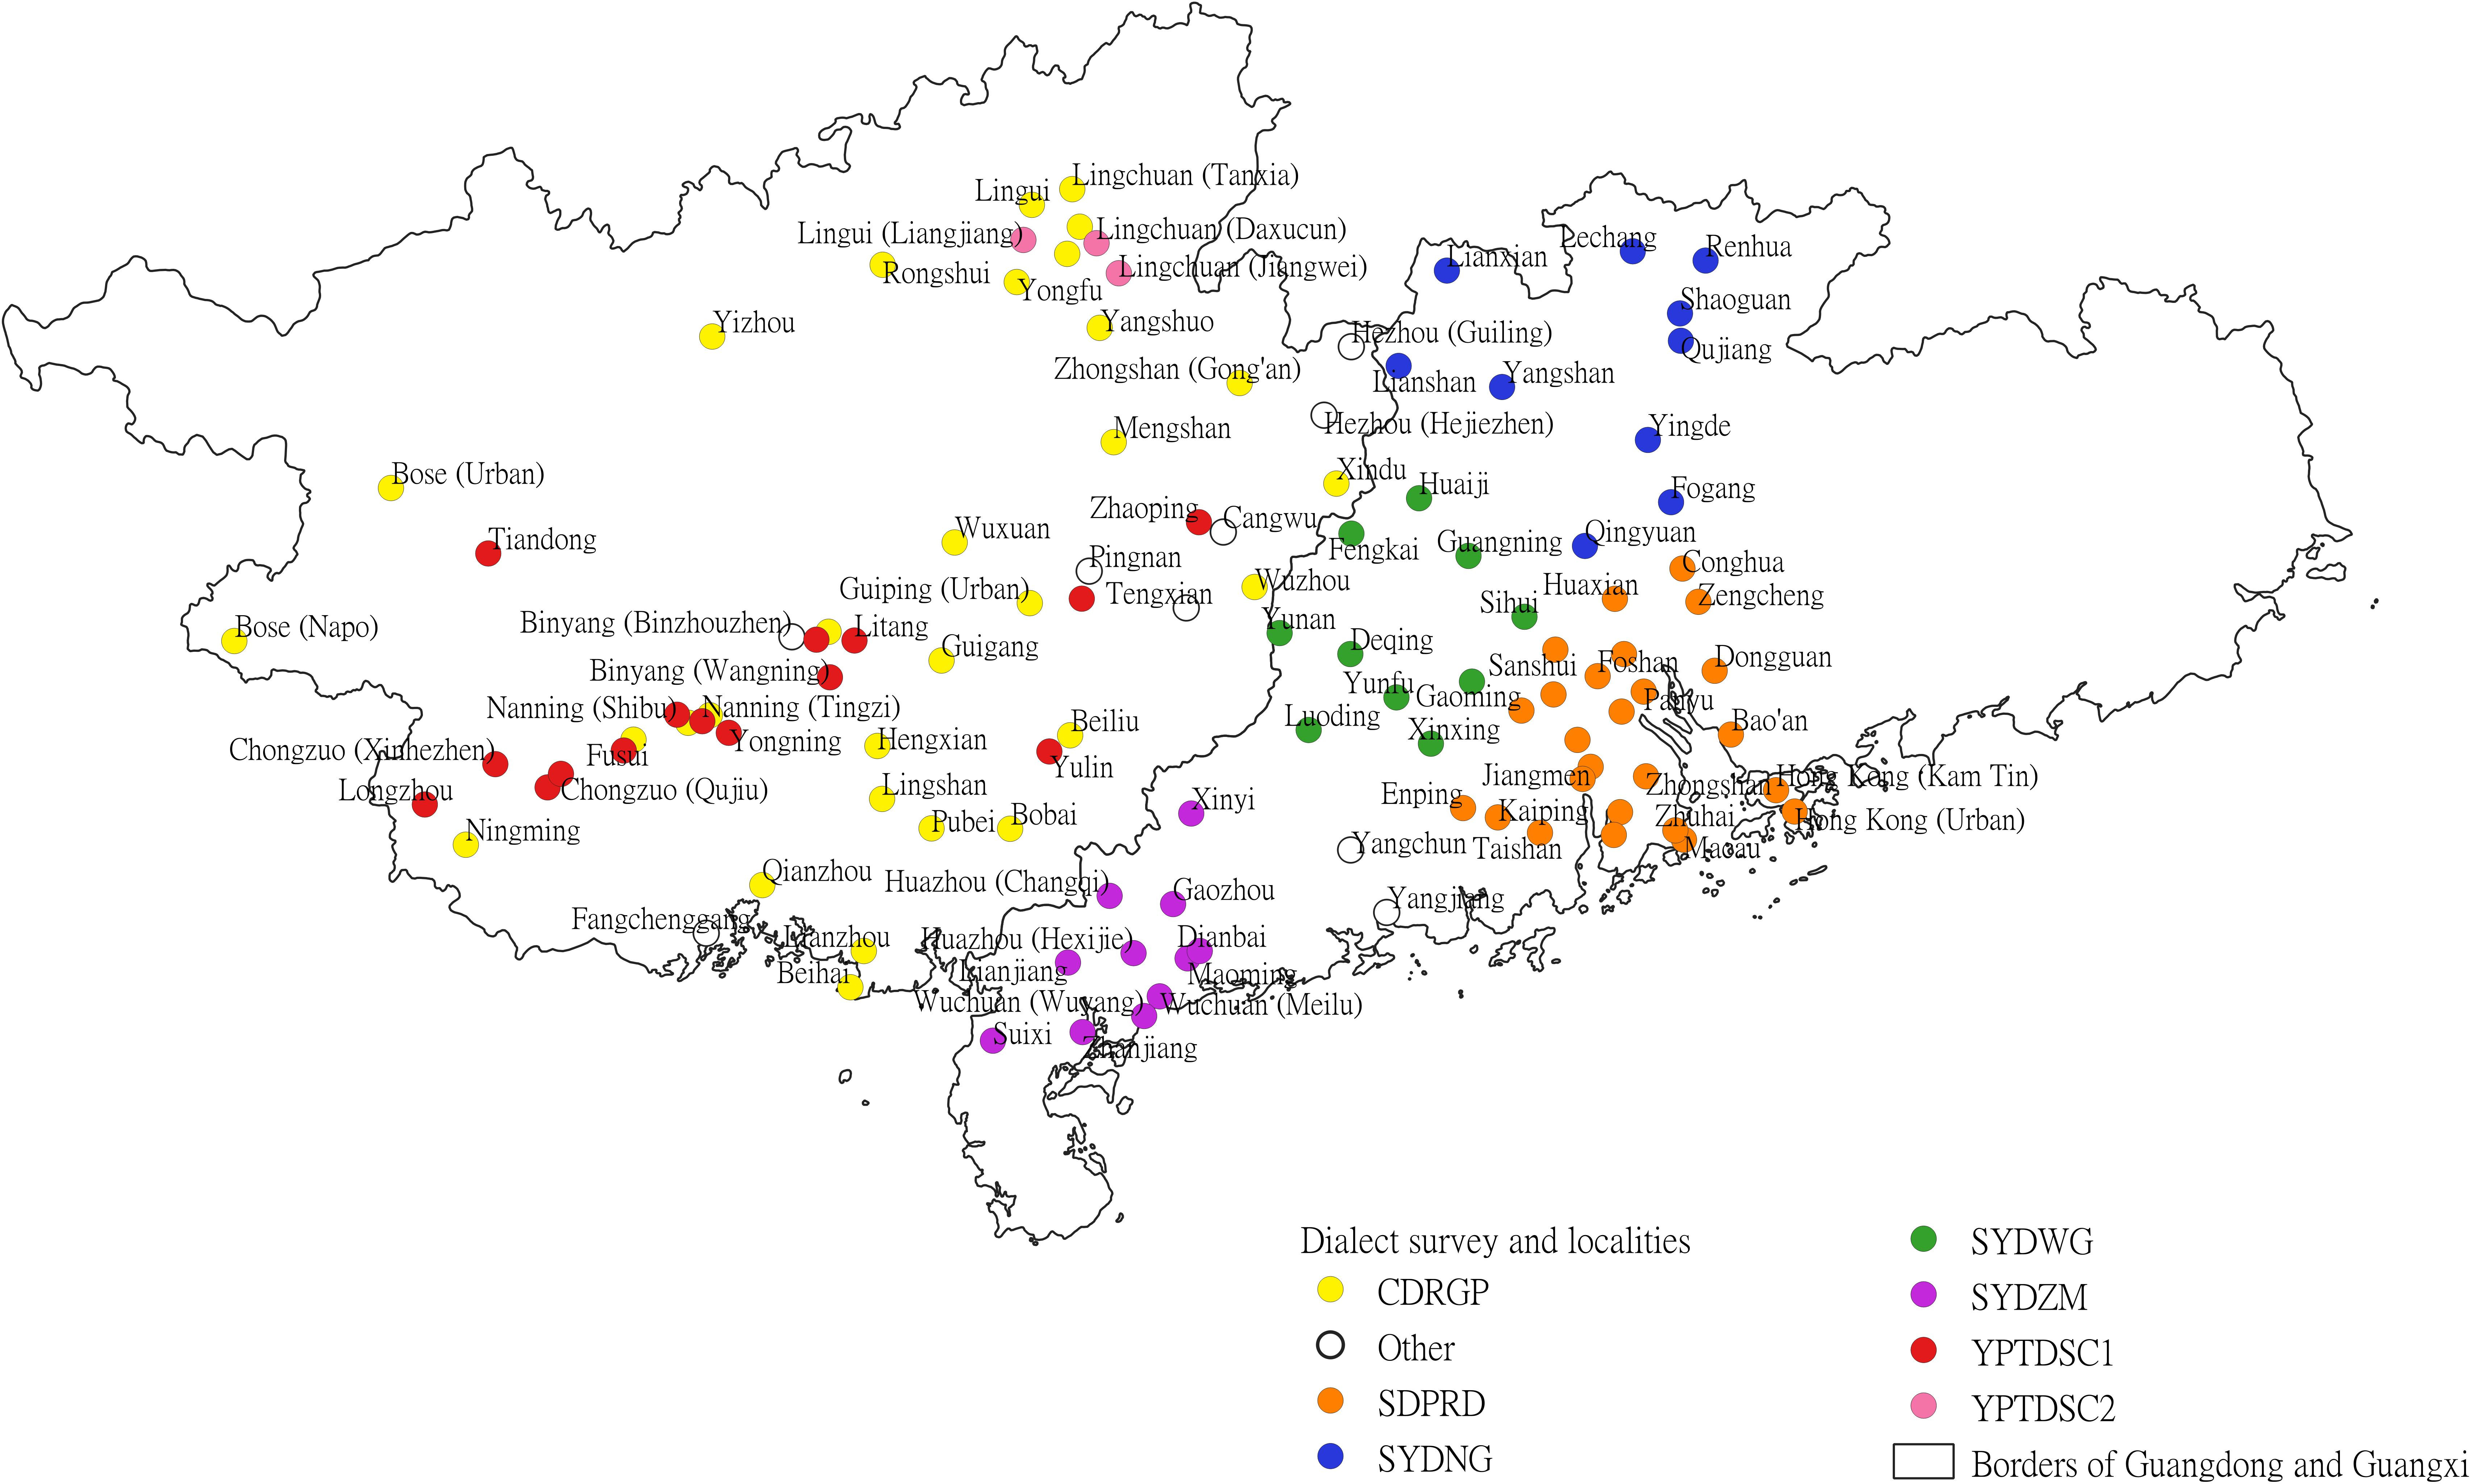
\includegraphics[width=\textwidth]{sung-img003.jpeg}
\caption{Localities and their respective sources}
\label{fig:sung:3}
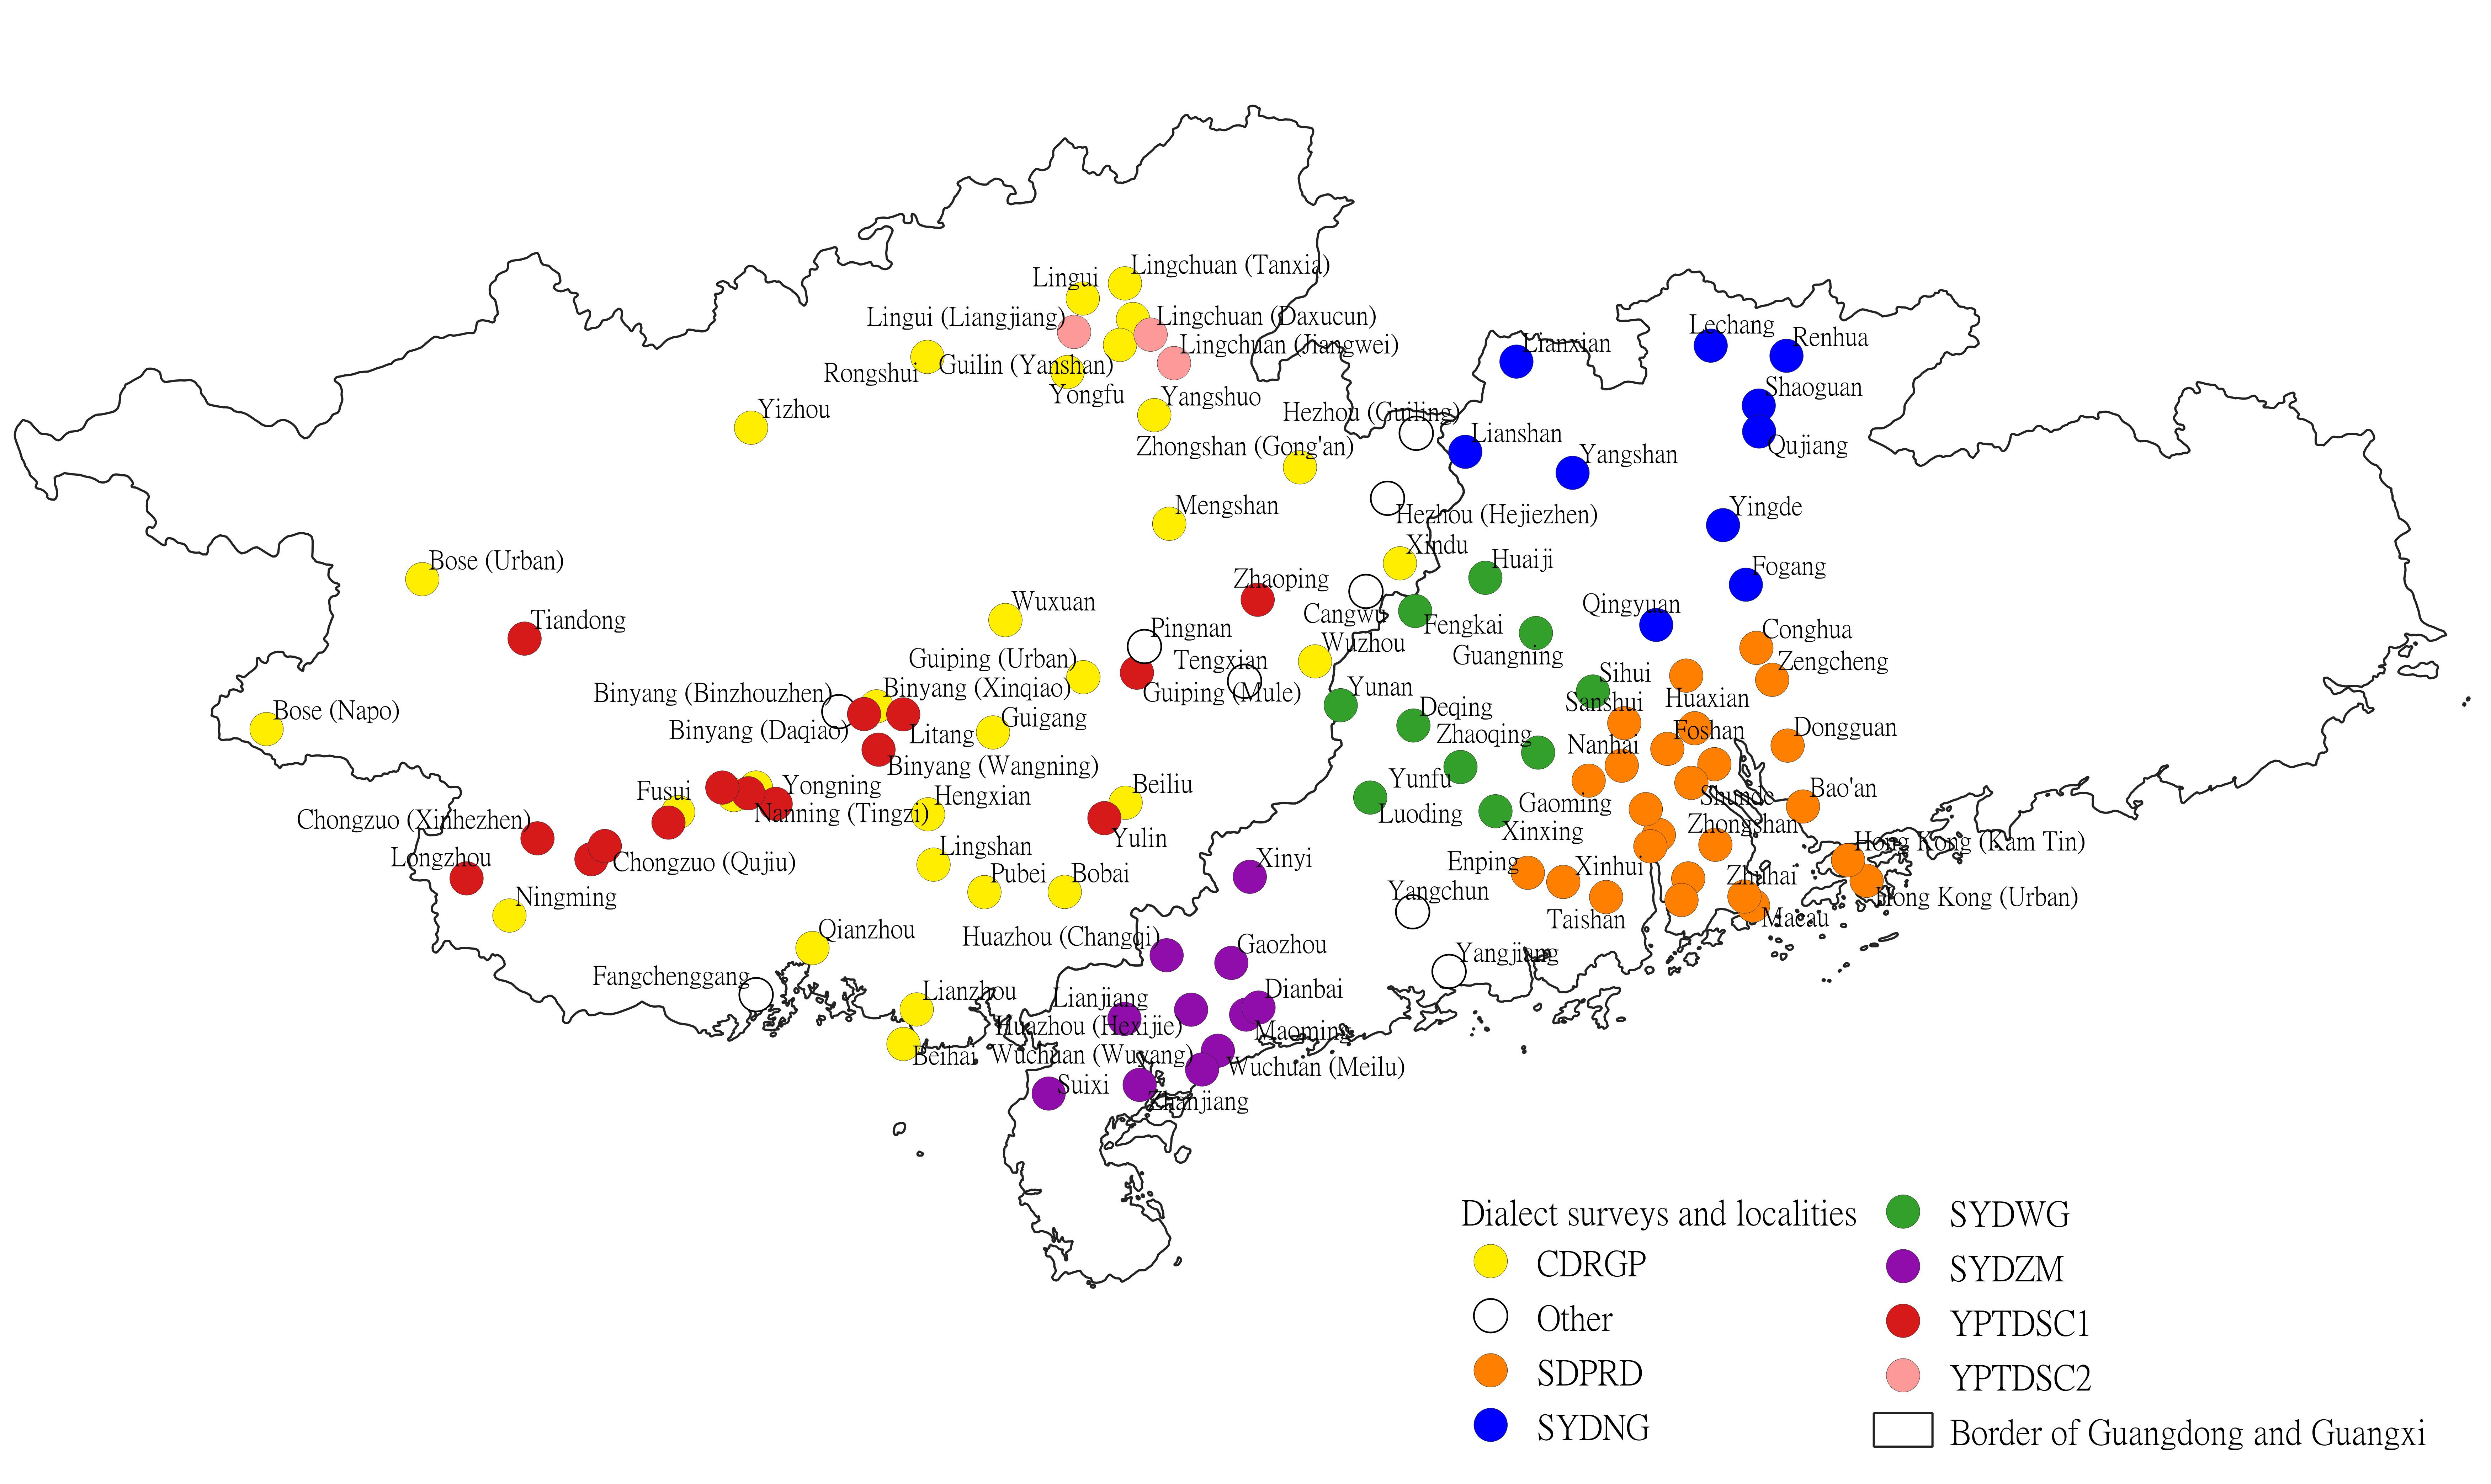
\includegraphics[width=\textwidth]{20240810 grafiken sung neu/Figure 3_locality_map_update_August2024.jpeg}
\end{figure}

Around 130 (monosyllabic) words\footnote{The word list is based on around 80 words from the Swadesh list, and the rest consists common words include an expansion in the domain of numbers, animals, directions, colours, as well as items which contain some notable Yue phonological features. The additional items in complementary to the Swadesh list is used to balance out some missing features that are not found in the Swadesh list.} are extracted and digitized from the original sources. The exact number of words per variety in the database varies as not every dialect contains the same number of transcribed words. The database contains 104 Yue and Southern Pinghua varieties (after removing the Northern Pinghua localities).

\subsection{Methodology}
\label{sec:sung:4.2}
We evaluate each tone distance measures based on i) number of tones distinguished, ii) comparison with perceptual dimensions (\citealt{GandourHarshman1978}), iii) local incoherence, iv) comparison with traditional classification, and v) comparison with segmental classification (dialectometry).

An ideal tone distance measure is able to distinguish all the tones found in the data. By computing the distances between all the tones in the data, we can visualize these distances on an MDS plot, and inspect how much overlap there is between the converted tone representations, i.e. how much do tones share the same representation under each method.  We also interpret the first two dimensions and check whether they match \citegen{GandourHarshman1978} perceptual dimensions of tones. Previous studies in dialectometry have validated their methods through comparing the linguistic distances with perceptual distances (e.g. \citealt{GooskensHeeringa2004}) and we apply the same approach in this study. For tones, \citet{GandourHarshman1978} and \citet{Gandour1983} have repeatedly found average pitch and direction as the most important dimensions in tone distance perception of native speakers from several tone languages. An ideal tone distance measure should also yield similar dimensions in the tone distances that each method produces.

Local incoherence is another external validation method used in dialectometry. Previous studies have shown that dialects closer to each other tend to be more similar than distant ones (the \textit{Fundamental Dialectological Postulate}, \citealt{NerbonneKleiweg2007}). This pattern has been found not only within dialectal variation, but also in other domains (in Geography, it is known as \textit{Tobler’s First Law of Geography}, \citealt{Tobler1970}). The idea behind local incoherence is to measure how much dialectal variation (in terms of the distances between the nearest dialects in any locality) matches the tendency stated above, when using a particular method. Since the optimal score is 0, a tone distance calculation method that gets a small local incoherence score is considered as a more suitable method.
\largerpage
Lastly, we want to know how similar or different the classifications generated by each method compare to the traditional and segmental classifications (from segmental dialectometry). The comparison can inform us whether tones behave similarly to segments as well as whether tones were used in the classification of dialects in the LAC \citep{CASS2012}, which may not have been explicitly stated. 

The comparison between the tonal classifications and the traditional classification or the segmental classification requires additional steps. Firstly, cluster analysis (Ward’s method) was performed on the segmental classification as well as the classification for each tone distance measure. The traditional classification in the \textit{Language Atlas of China} originally gives ten different groups. However, in our dataset one of them consists of only two dialects (Suixi and Litang under ‘Unclassified'\footnote{The LAC did not include this locality in their classification.}; the other two groups consist of one dialect (Huazhou (Hexijie) under ‘Wuhua’) and Lingui under 'Guibei Pinghua'). We have merged these two dialects with the Gaoyang dialect group, whereas Litang and Lingui now group with Guinan Pinghua, based on their geographical proximity in order to avoid clusters consisting of only one element.

To compare the similarity of classification (dialect groups) between each cluster solution, we have chosen to use the Adjusted Rand Index as an indicator to measure how much each cluster overlaps between a Reference Classification and an Observed Solution.\footnote{In the literature, the reference classification is known as the Gold Standard. However, since the classifications we are using are not the absolute correct solution in our context (since there is no one ‘correct’ solution in dialectology), we use an alternate name instead.} The Adjusted Rand Index (ARI hereafter) is a method used for comparing two different clustering solutions (with chance correction, \citealt{HubertArabie1985}), which derived from the Rand Index \citep{Rand1971}. We are assuming that the traditional classification and the segmental classification are Reference Classifications, and the classification generated with each tone distance measure are the Observed Solutions, which are compared against the Reference Classification. If two classifications completely overlap, the score is 1, if they only overlap on the chance level, the score is 0. We are using the ARI scores for the comparison instead of regression for the following reasons. Firstly, the classification in the LAC is not empirically supported, which means we do not have a solid classification to compare to yet (see \sectref{sec:sung:3.1}). This study also does not include a regression analysis to see how much each method can add to the explained variance to the segmental distances. Tones as a separate linguistic level has not been studied in dialectometry, and this current study aims to fill this gap.

The classification maps for the Reference classification and each of the tone distance measure can be found in the appendix.

\section{Results}
\label{sec:sung:5}
As described in \sectref{sec:sung:2}, there are 4 tone distance measures that are found in the literature which are also easy to replicate. Firstly, we calculate the pairwise distances between all the dialects by calculating the tone distances for each lexical item (see \sectref{sec:sung:2} for the details of each method). We then calculate the aggregate pairwise distance between each dialect in the data by summing all the lexical tone distances divided by the total number of comparisons in the pair. This procedure is repeated for all the dialects in the data. For each method, the aggregate pairwise distances are stored in a distance matrix. These matrices are then used for the further analyses in the following sub-sections.

\subsection{Tone overlap and perceptual dimensions}
\label{sec:sung:5.1}
   
\begin{figure}
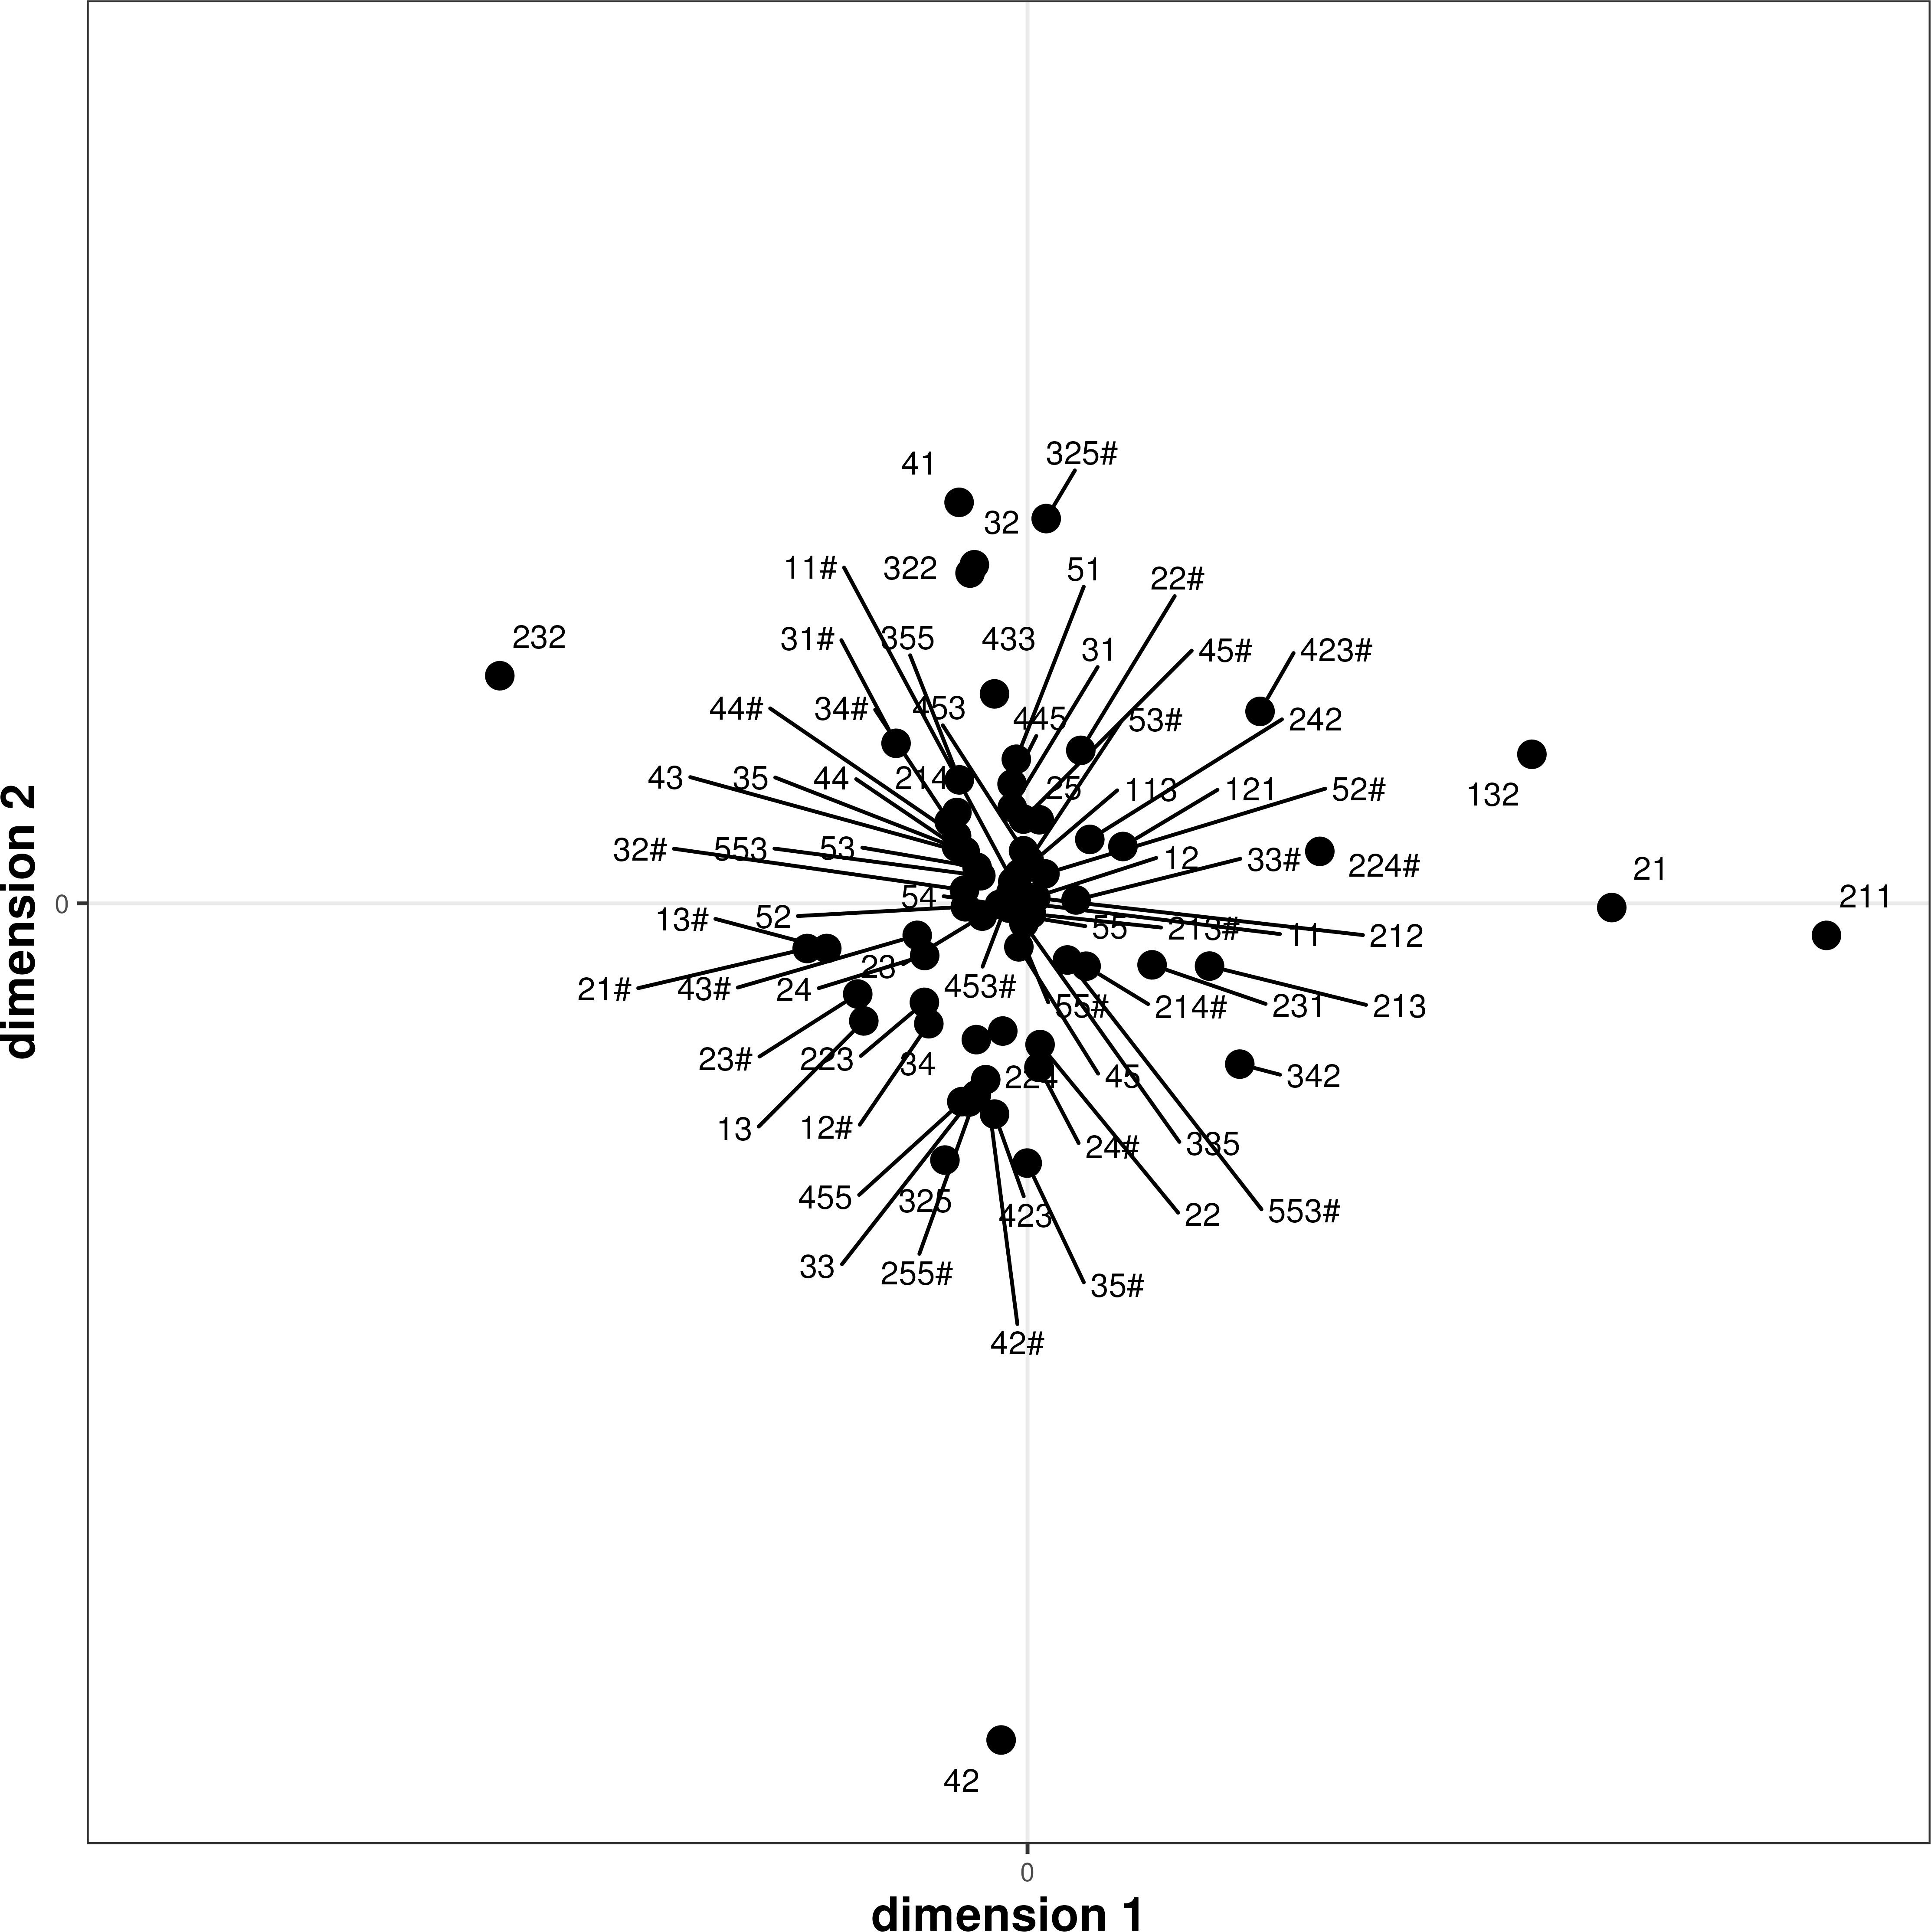
\includegraphics[width=\textwidth]{sung-img004a.PNG}
\caption{\label{fig:sung:4a}MDS plot for Binary comparisons (Classic MDS), r\textsuperscript{2} = n.a.}
\end{figure}

In this section, we will present Multidimensional Scaling (MDS) plots to visualize the distances between all the tones in the Yue data under different tone distance calculation methods introduced in \sectref{sec:sung:2}. MDS is a dimension reduction method which represents “measurements of similarity (or dissimilarity) among pairs of objects as distances between points in a low-dimension multidimensional space” (\citealt{BorgGroenen2005}: 3). In our case, an MDS plot would represent the distances between tones (represented by labelled points in the plot), and the further the points are from each other, the more different they are. The MDS plots for the tone distances calculated using each method are shown from Figures~\ref{fig:sung:4a}--\ref{fig:sung:7}.\footnote{Plots and explained variances were produced and calculated with \textit{LED-A} \citep{HeeringaEtAl2022}, except \figref{fig:sung:7}.}  Note that unless specified, the classical MDS has been used in the analysis.

   
\begin{figure}
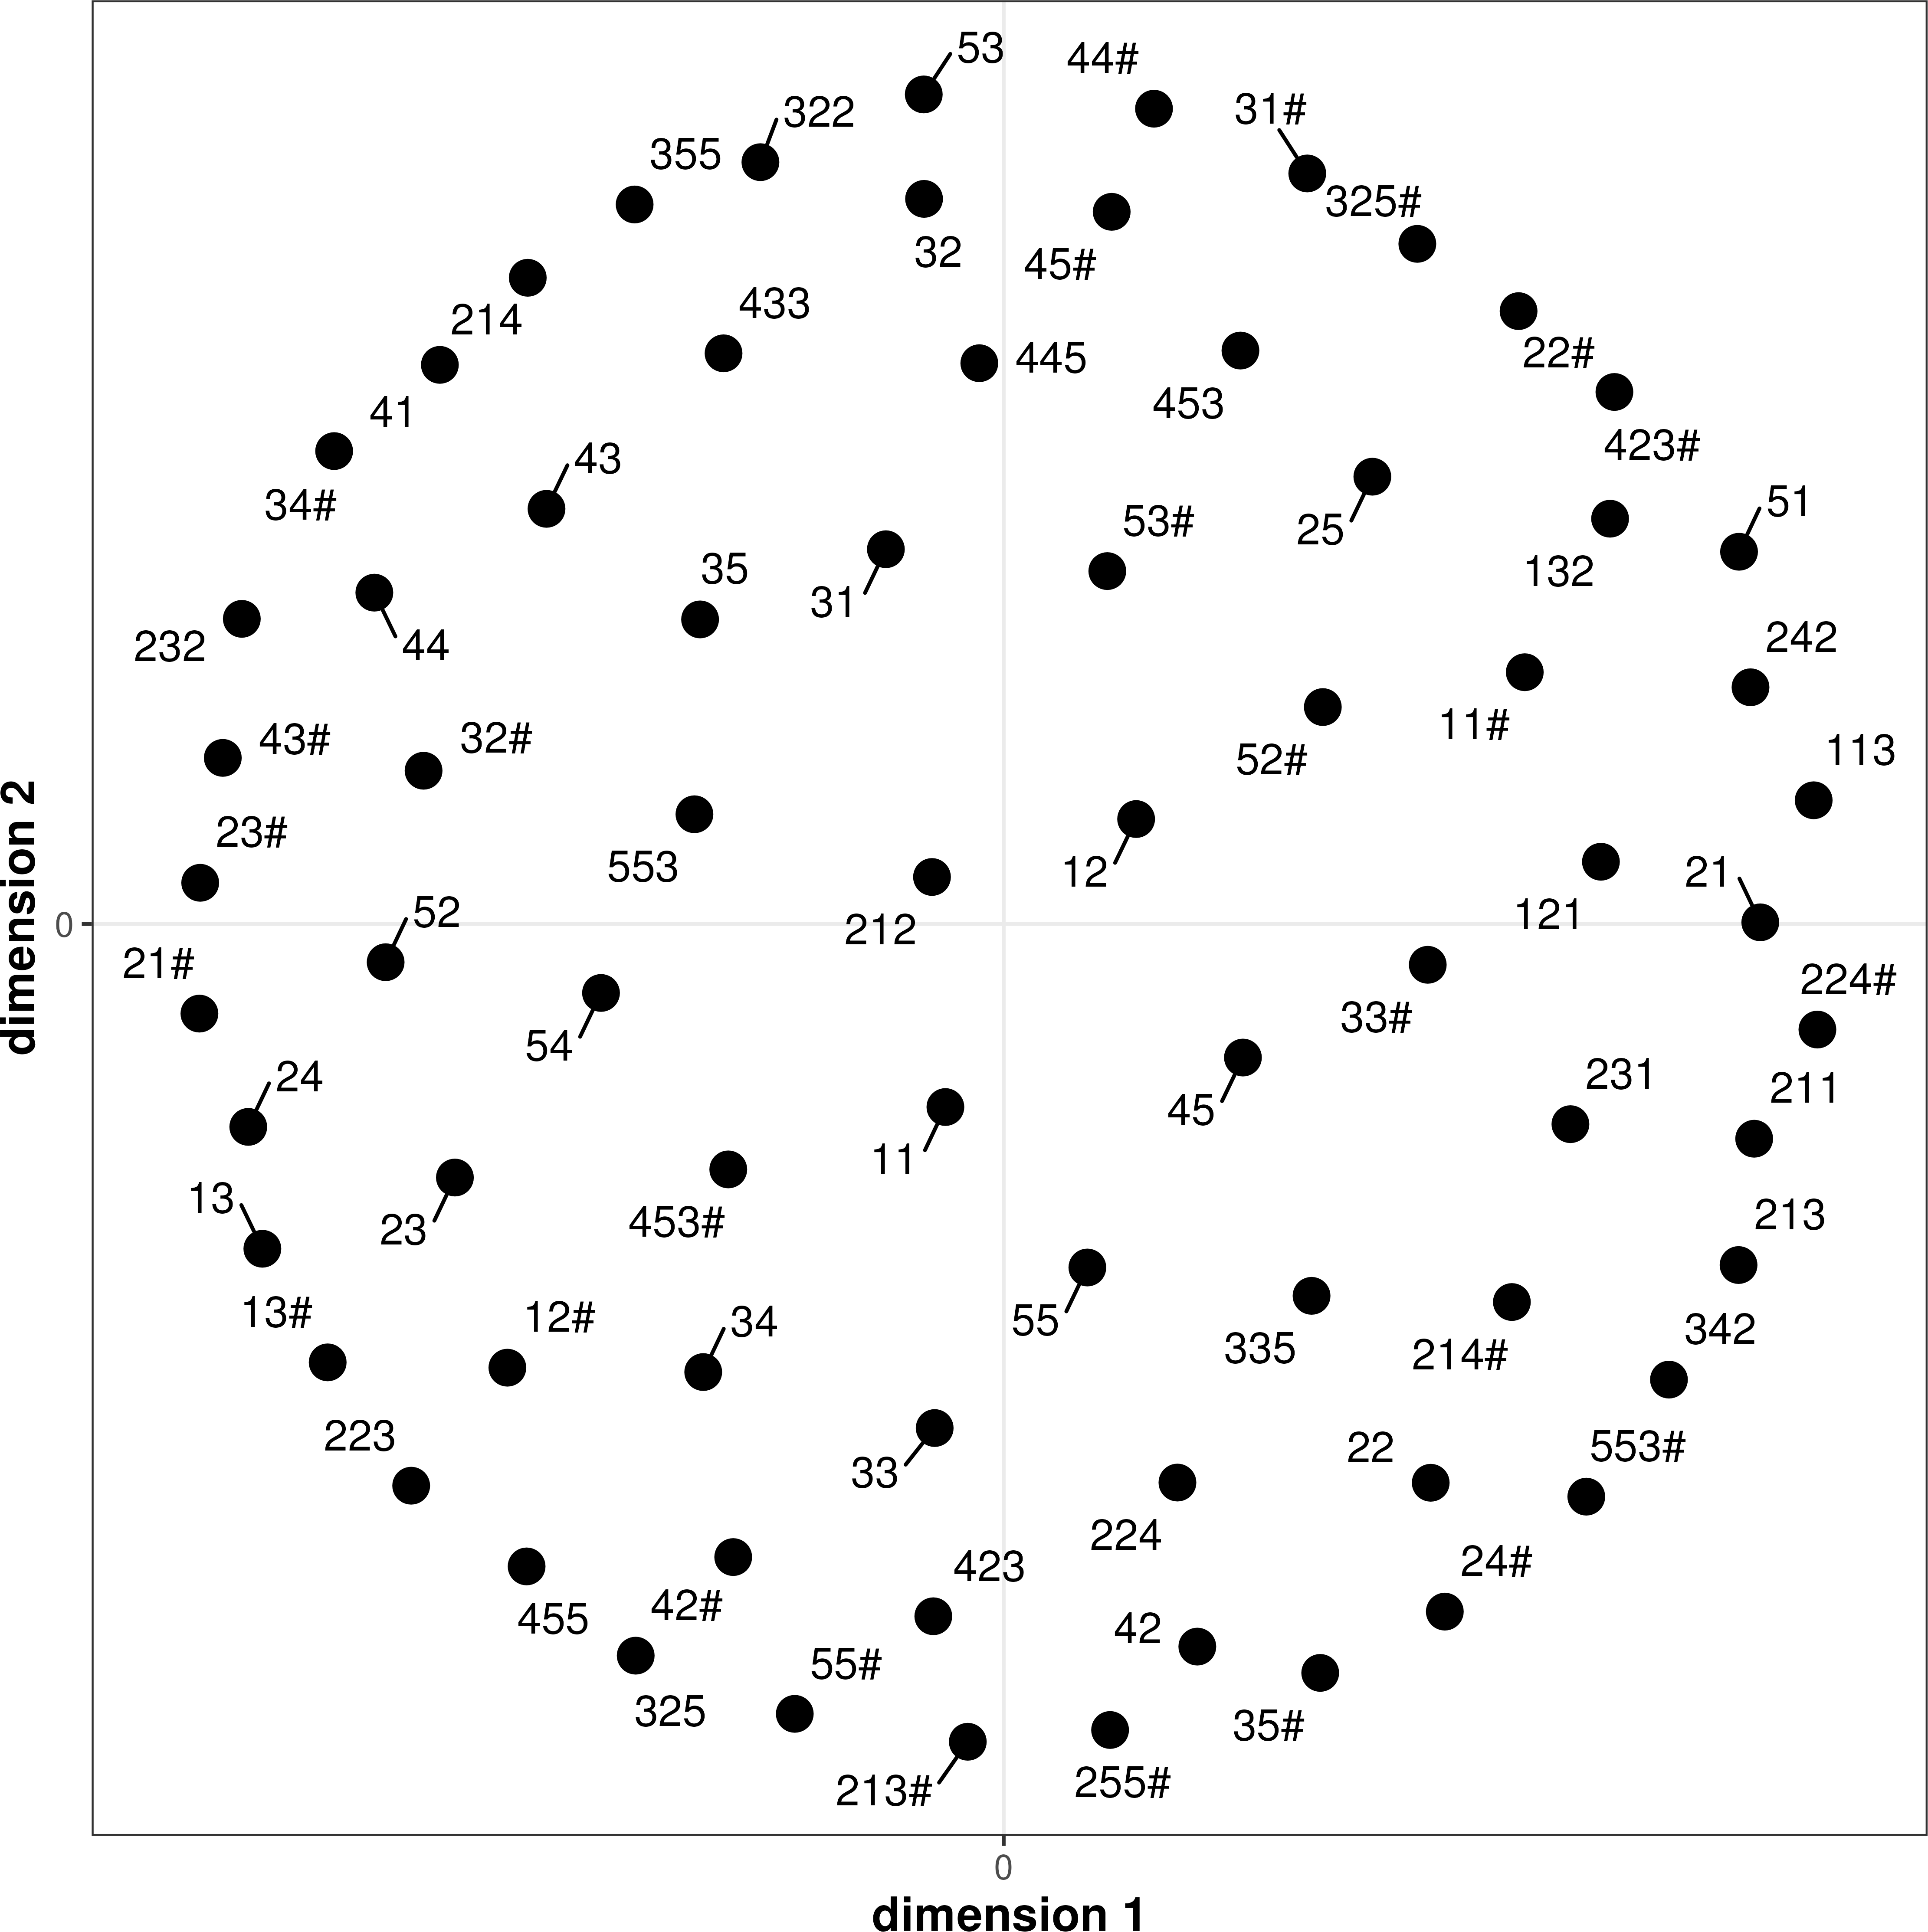
\includegraphics[width=\textwidth]{sung-img004b.PNG}
\caption{\label{fig:sung:4b} MDS plot for Binary comparisons (Sammon’s MDS), r\textsuperscript{2} = n.a.}
\end{figure}

The first evaluation on the tone distance calculation methods is based on the number of overlapping representations of tones in the dataset. An MDS plot is useful in visualizing tone overlaps, which are indicated by the total number of dots in the plot and the additional lines pointing at each overlapping representation in each plot. \citet{GandourHarshman1978} and \citet{Gandour1983} used the same technique to extract perceptual dimensions.

   
\begin{figure}
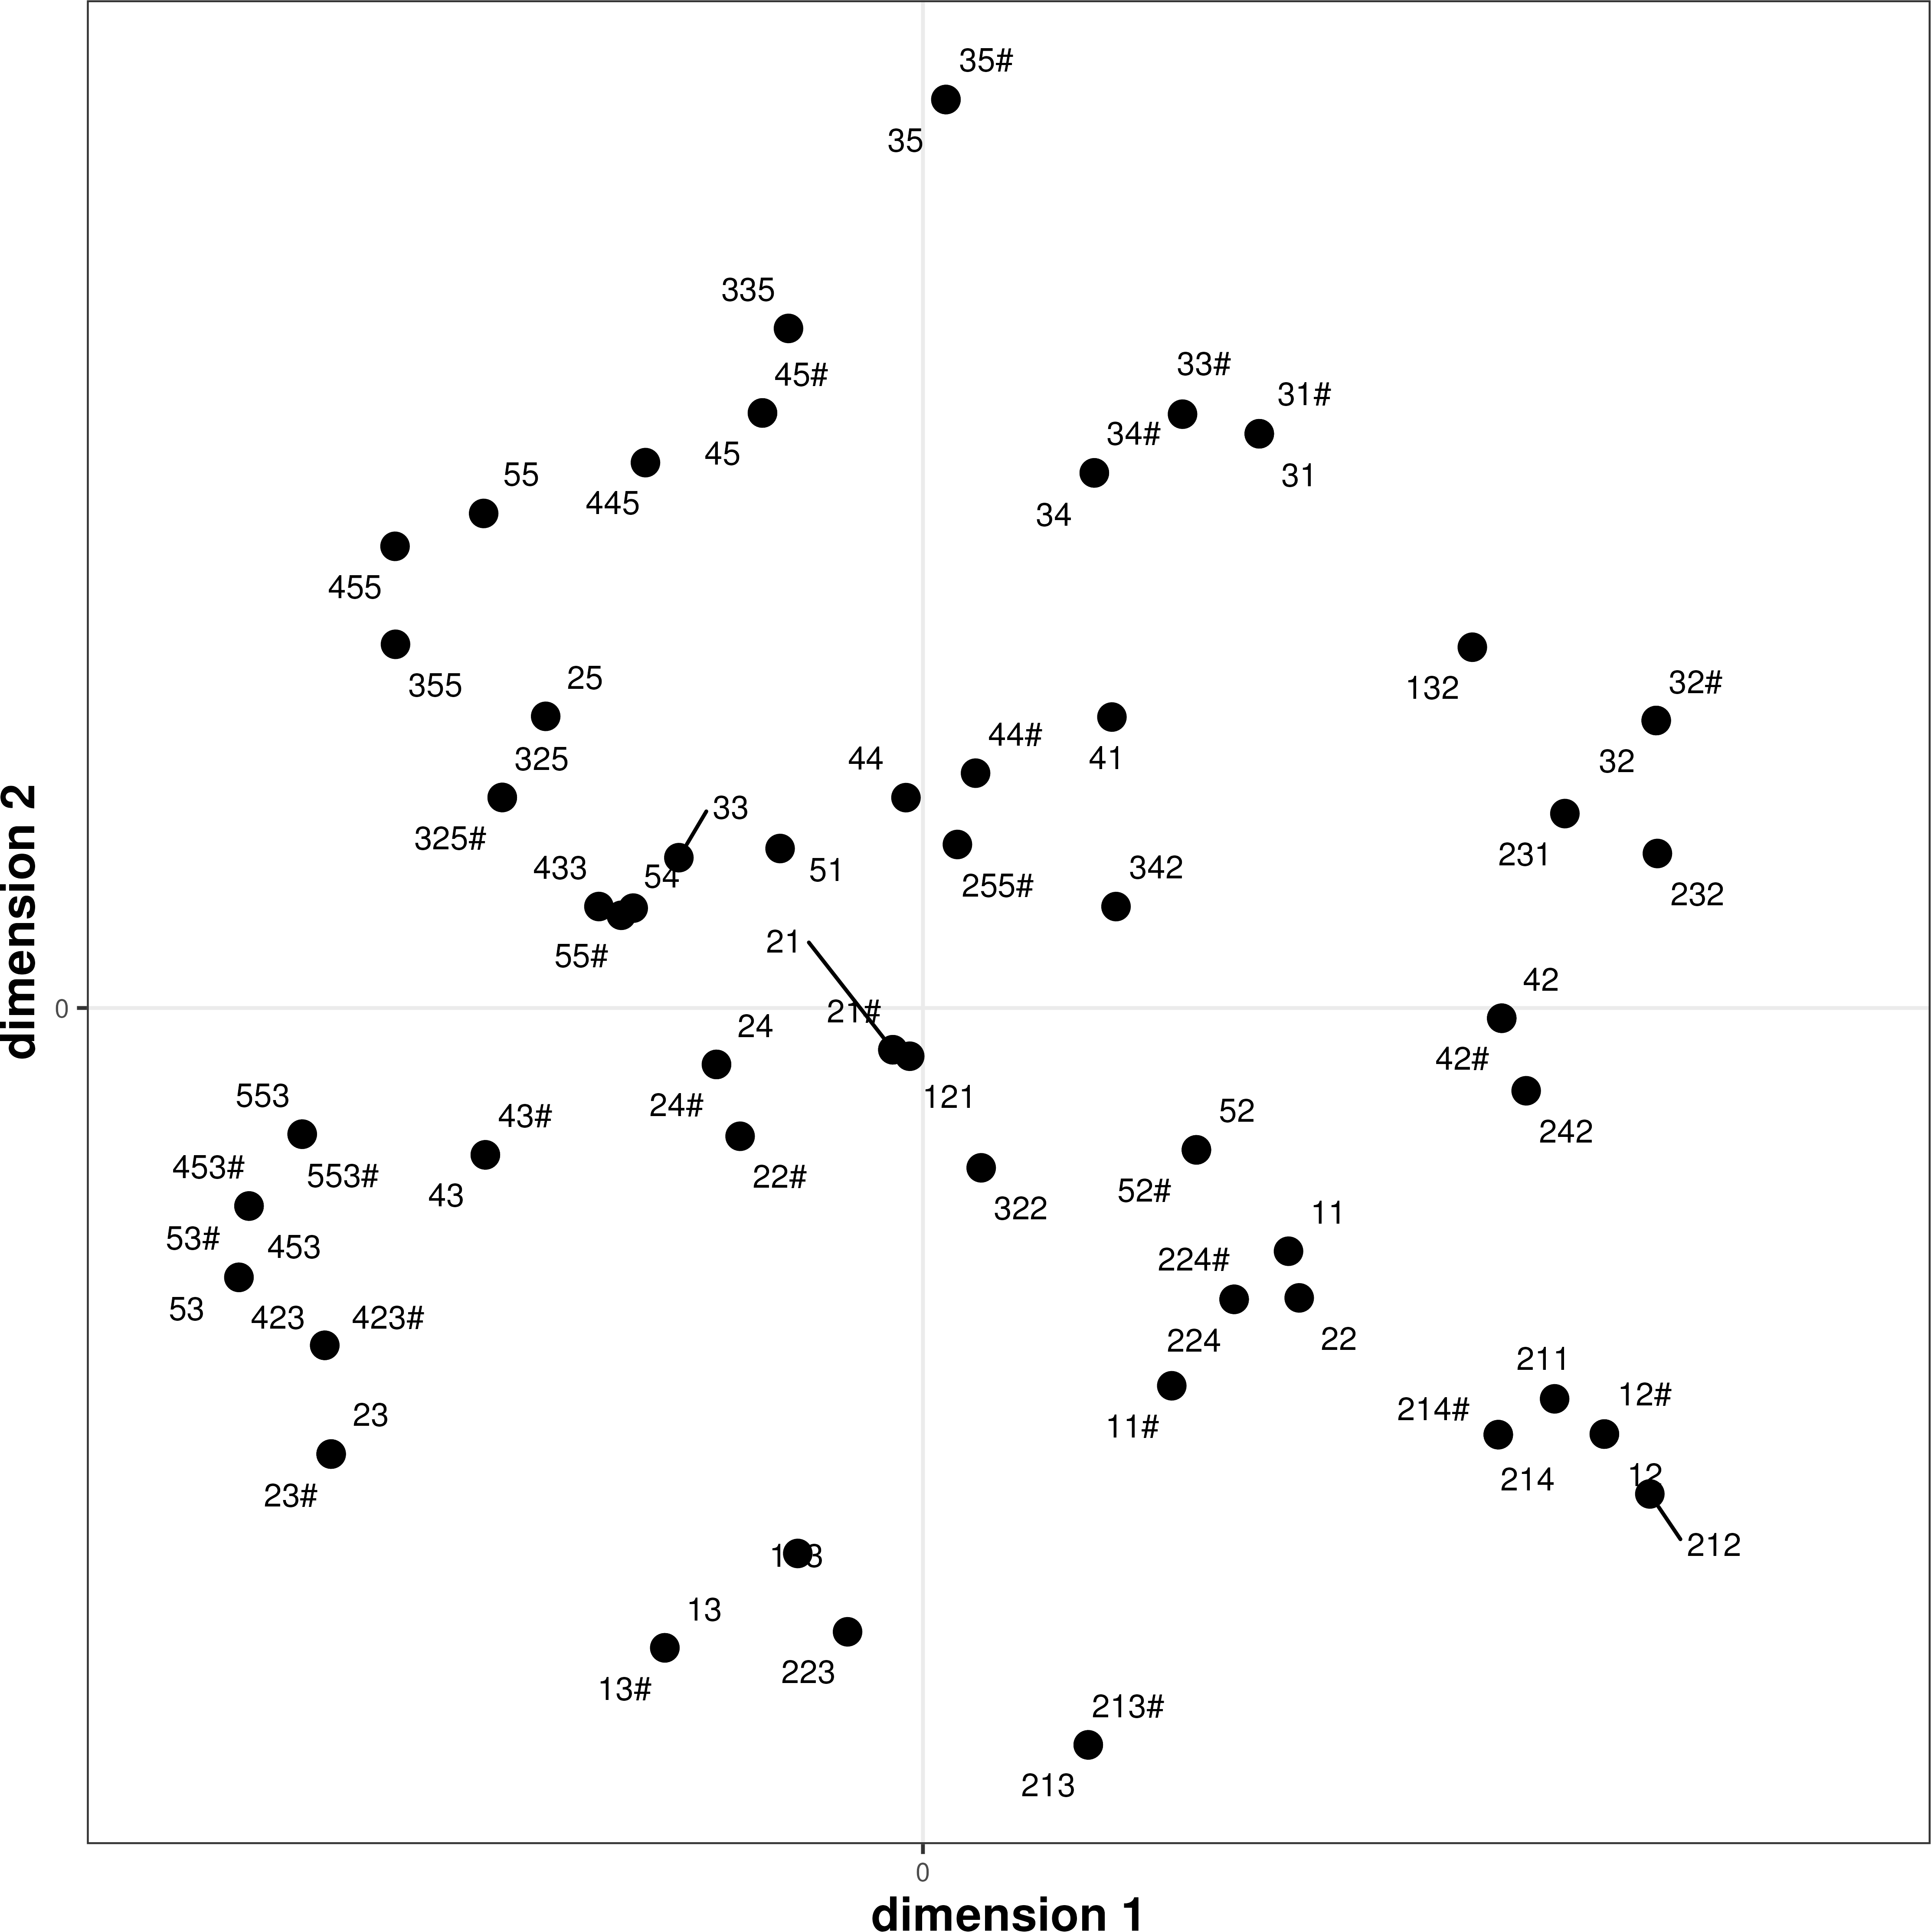
\includegraphics[width=\textwidth]{sung-img005.PNG}
\caption{MDS plot for Tone-to-string, r\textsuperscript{2} = 0.26}
\label{fig:sung:5}
\end{figure}

\tabref{tab:sung:7} summarizes the number of tones each method distinguishes from the original dataset, in both raw token and percentage. The total number of distinctive tones in the data is 73.


\begin{table}
\begin{tabular}{lrr}
\lsptoprule
         & Tones & Distinction \\
{Method} & {differentiated} & {rate}\\\midrule
Binary & 73 & 100\%\\
Tone-to-string & 52 & 71.2\%\\
OCO & 32 & 43.8\%\\
GH-T & 40 & 54.8\%\\
\lspbottomrule
\end{tabular}
\caption{Differentiation of tones under each tone distance measure}
\label{tab:sung:7}
\end{table}

   
\begin{figure}
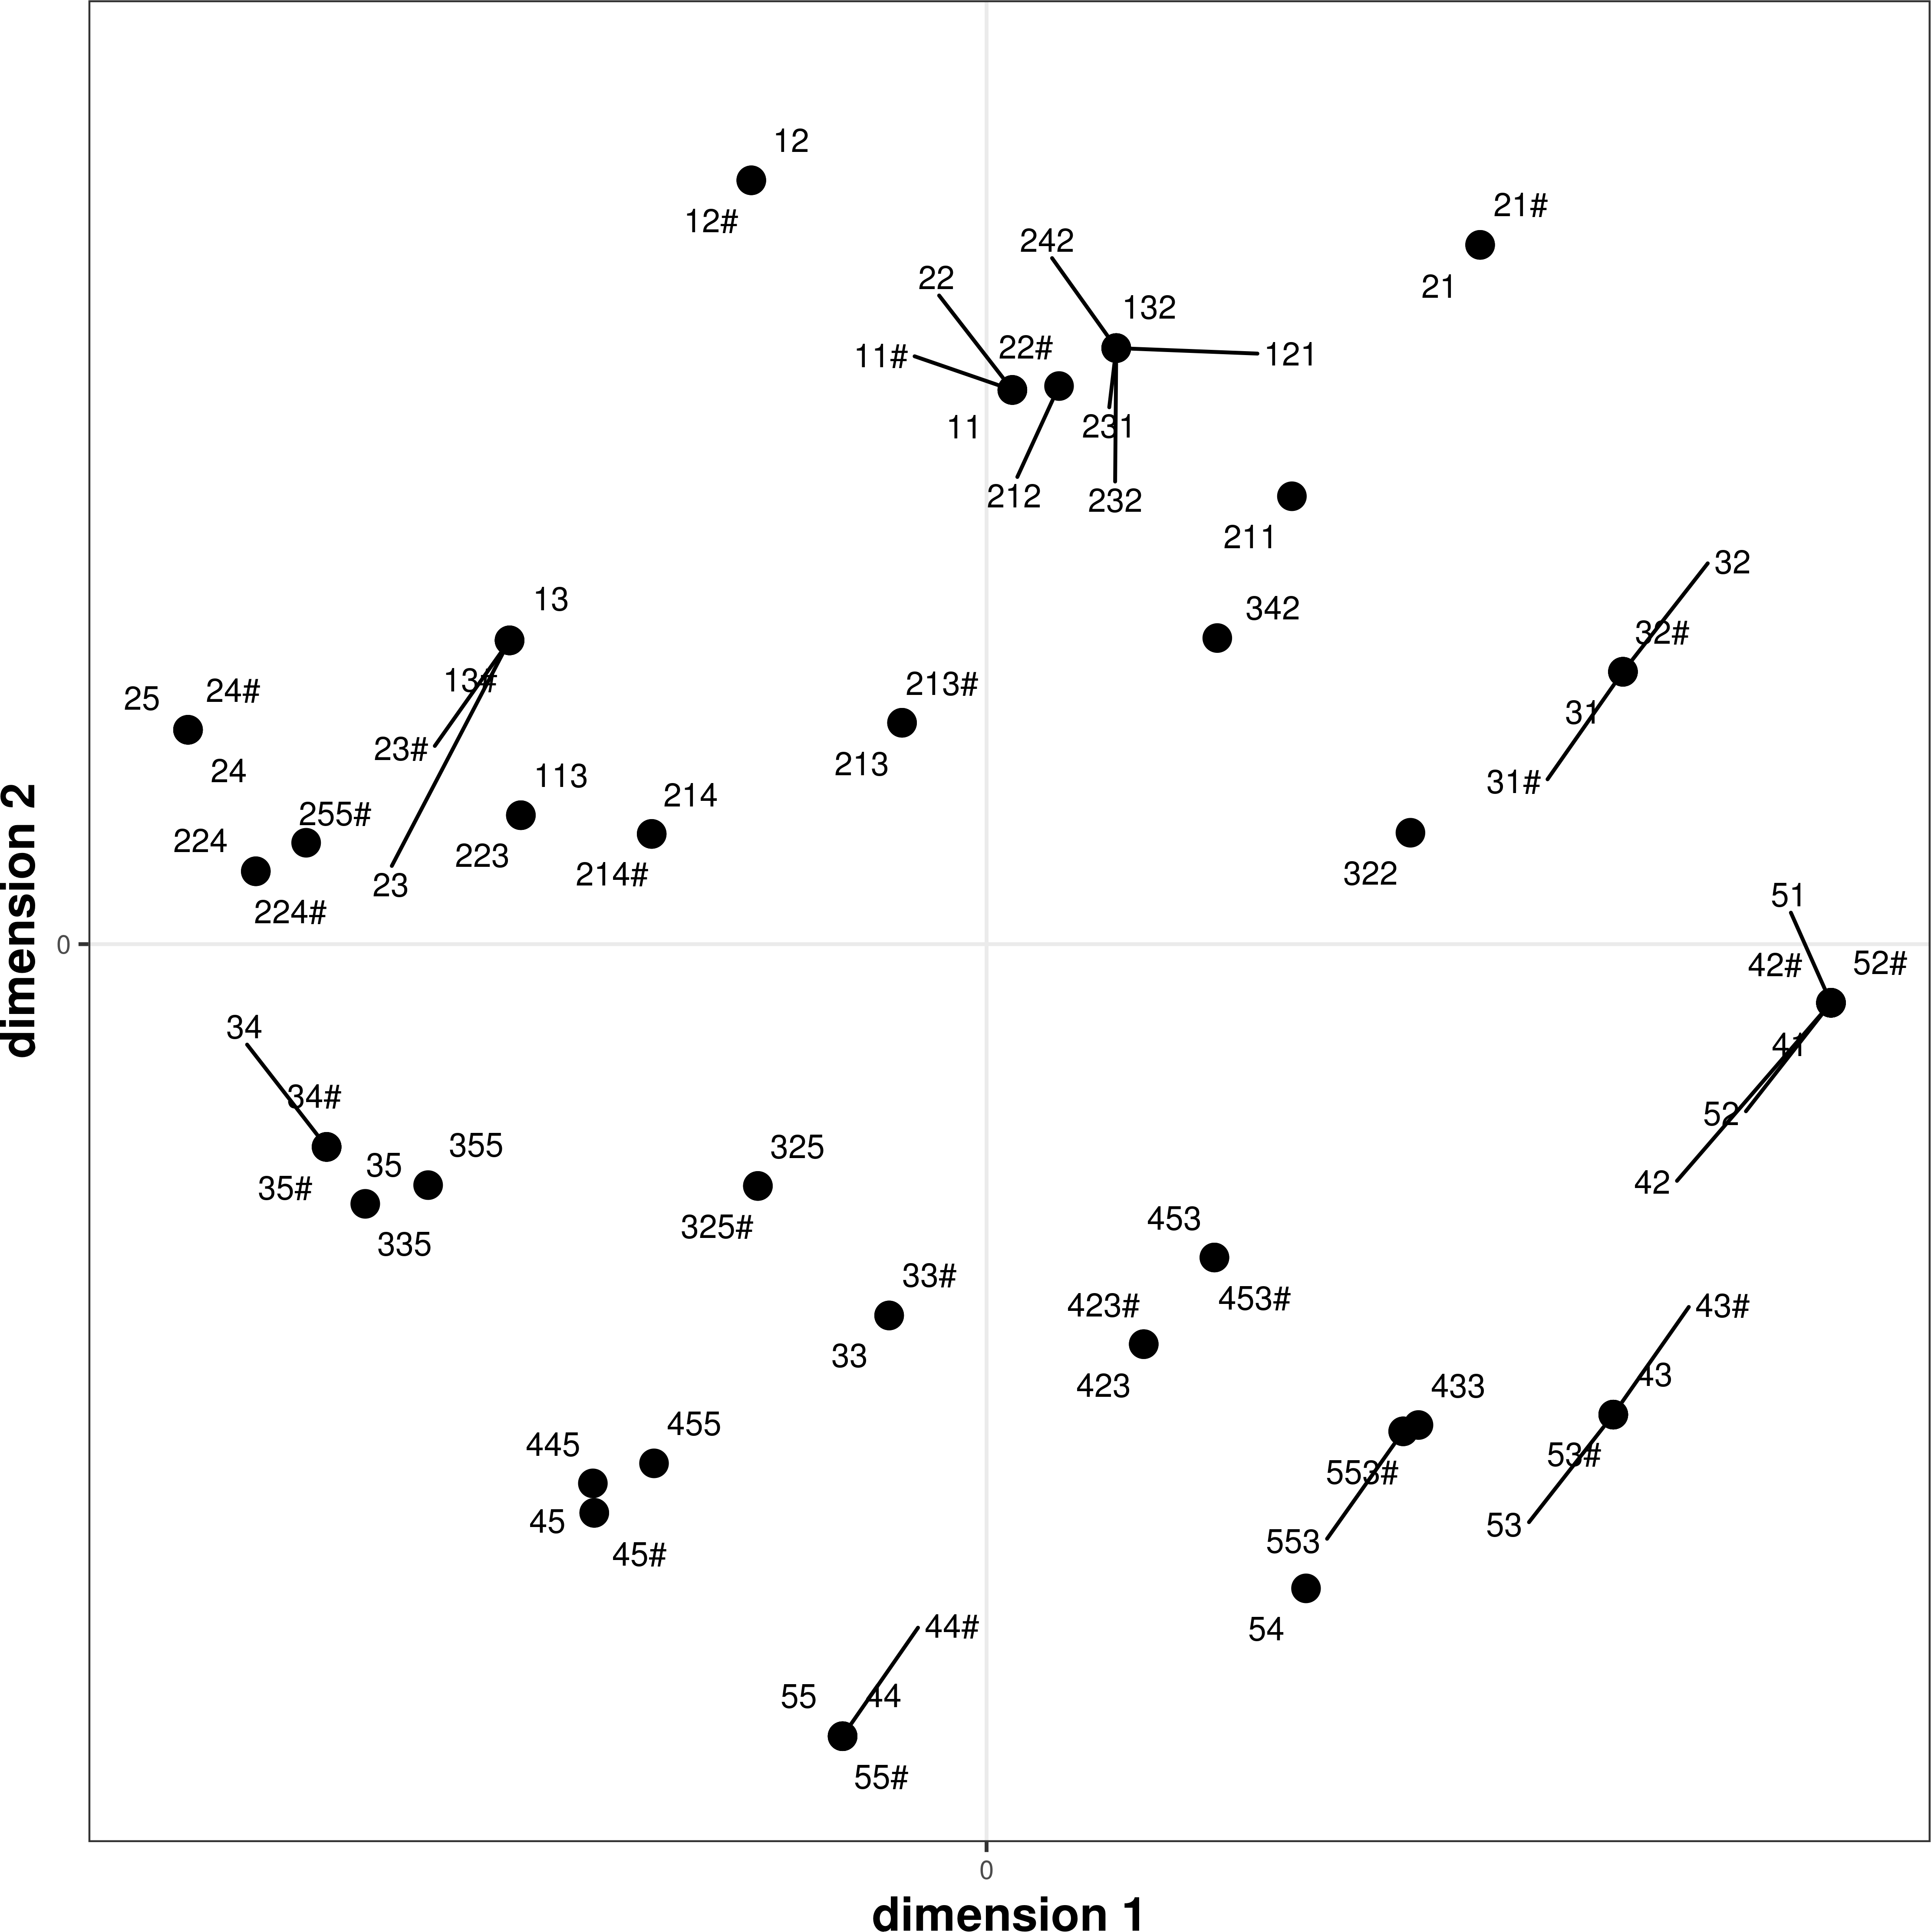
\includegraphics[width=\textwidth]{sung-img006.PNG}
\caption{MDS plot for OCO, r\textsuperscript{2} = 0.59}
\label{fig:sung:6}
\end{figure}

In \tabref{tab:sung:7}, we can see that the Binary method yields full distinction between all the tones in the data, and Tone-to-string can differentiate slightly over 70\% of the tones in the data. For GH-T, only 54.8\% of the tones can be differentiated, and lastly, OCO performs the poorest out of all methods, with under half of the tones in the data only.

The overlap of tones for the Tone-to-string method mainly occurs in cases where there is long and short distinction (indicated by the ‘\#’ in \figref{fig:sung:5}). Both \citet{YangCastro2008} and \citet{Tang2009} did not specify how they dealt with short phonetic tones, therefore, the current analysis has removed the short tone marker in the data. For the OCO method (\figref{fig:sung:6}), in addition to the lack of length distinction, the contrasts between several tones with similar contour have been collapsed. For example, we can see a cluster of six tones on the right consisting of 41, 42, 42\#, 51, 52, 52\# sharing the same OCO representation. This overlap is the result of collapsing a five-level contour transcription system into a three-level representation. Lastly, in the GH-T representation (\figref{fig:sung:7}), there are also overlapping tones with similar contours (e.g. the cluster at the top, consisting 42, 32, 43) or tones which share the same latter two digits (e.g. the cluster at the bottom consisting 23, 24, 224\#, 423\#). This is due to how tones are encoded with their features (see \tabref{tab:sung:5}) as well as how tones with two and three digits align (see \sectref{sec:sung:3.5}). A potential method in maximizing the distinctions of each method will be discussed in \sectref{sec:sung:5}.

  
\begin{figure}
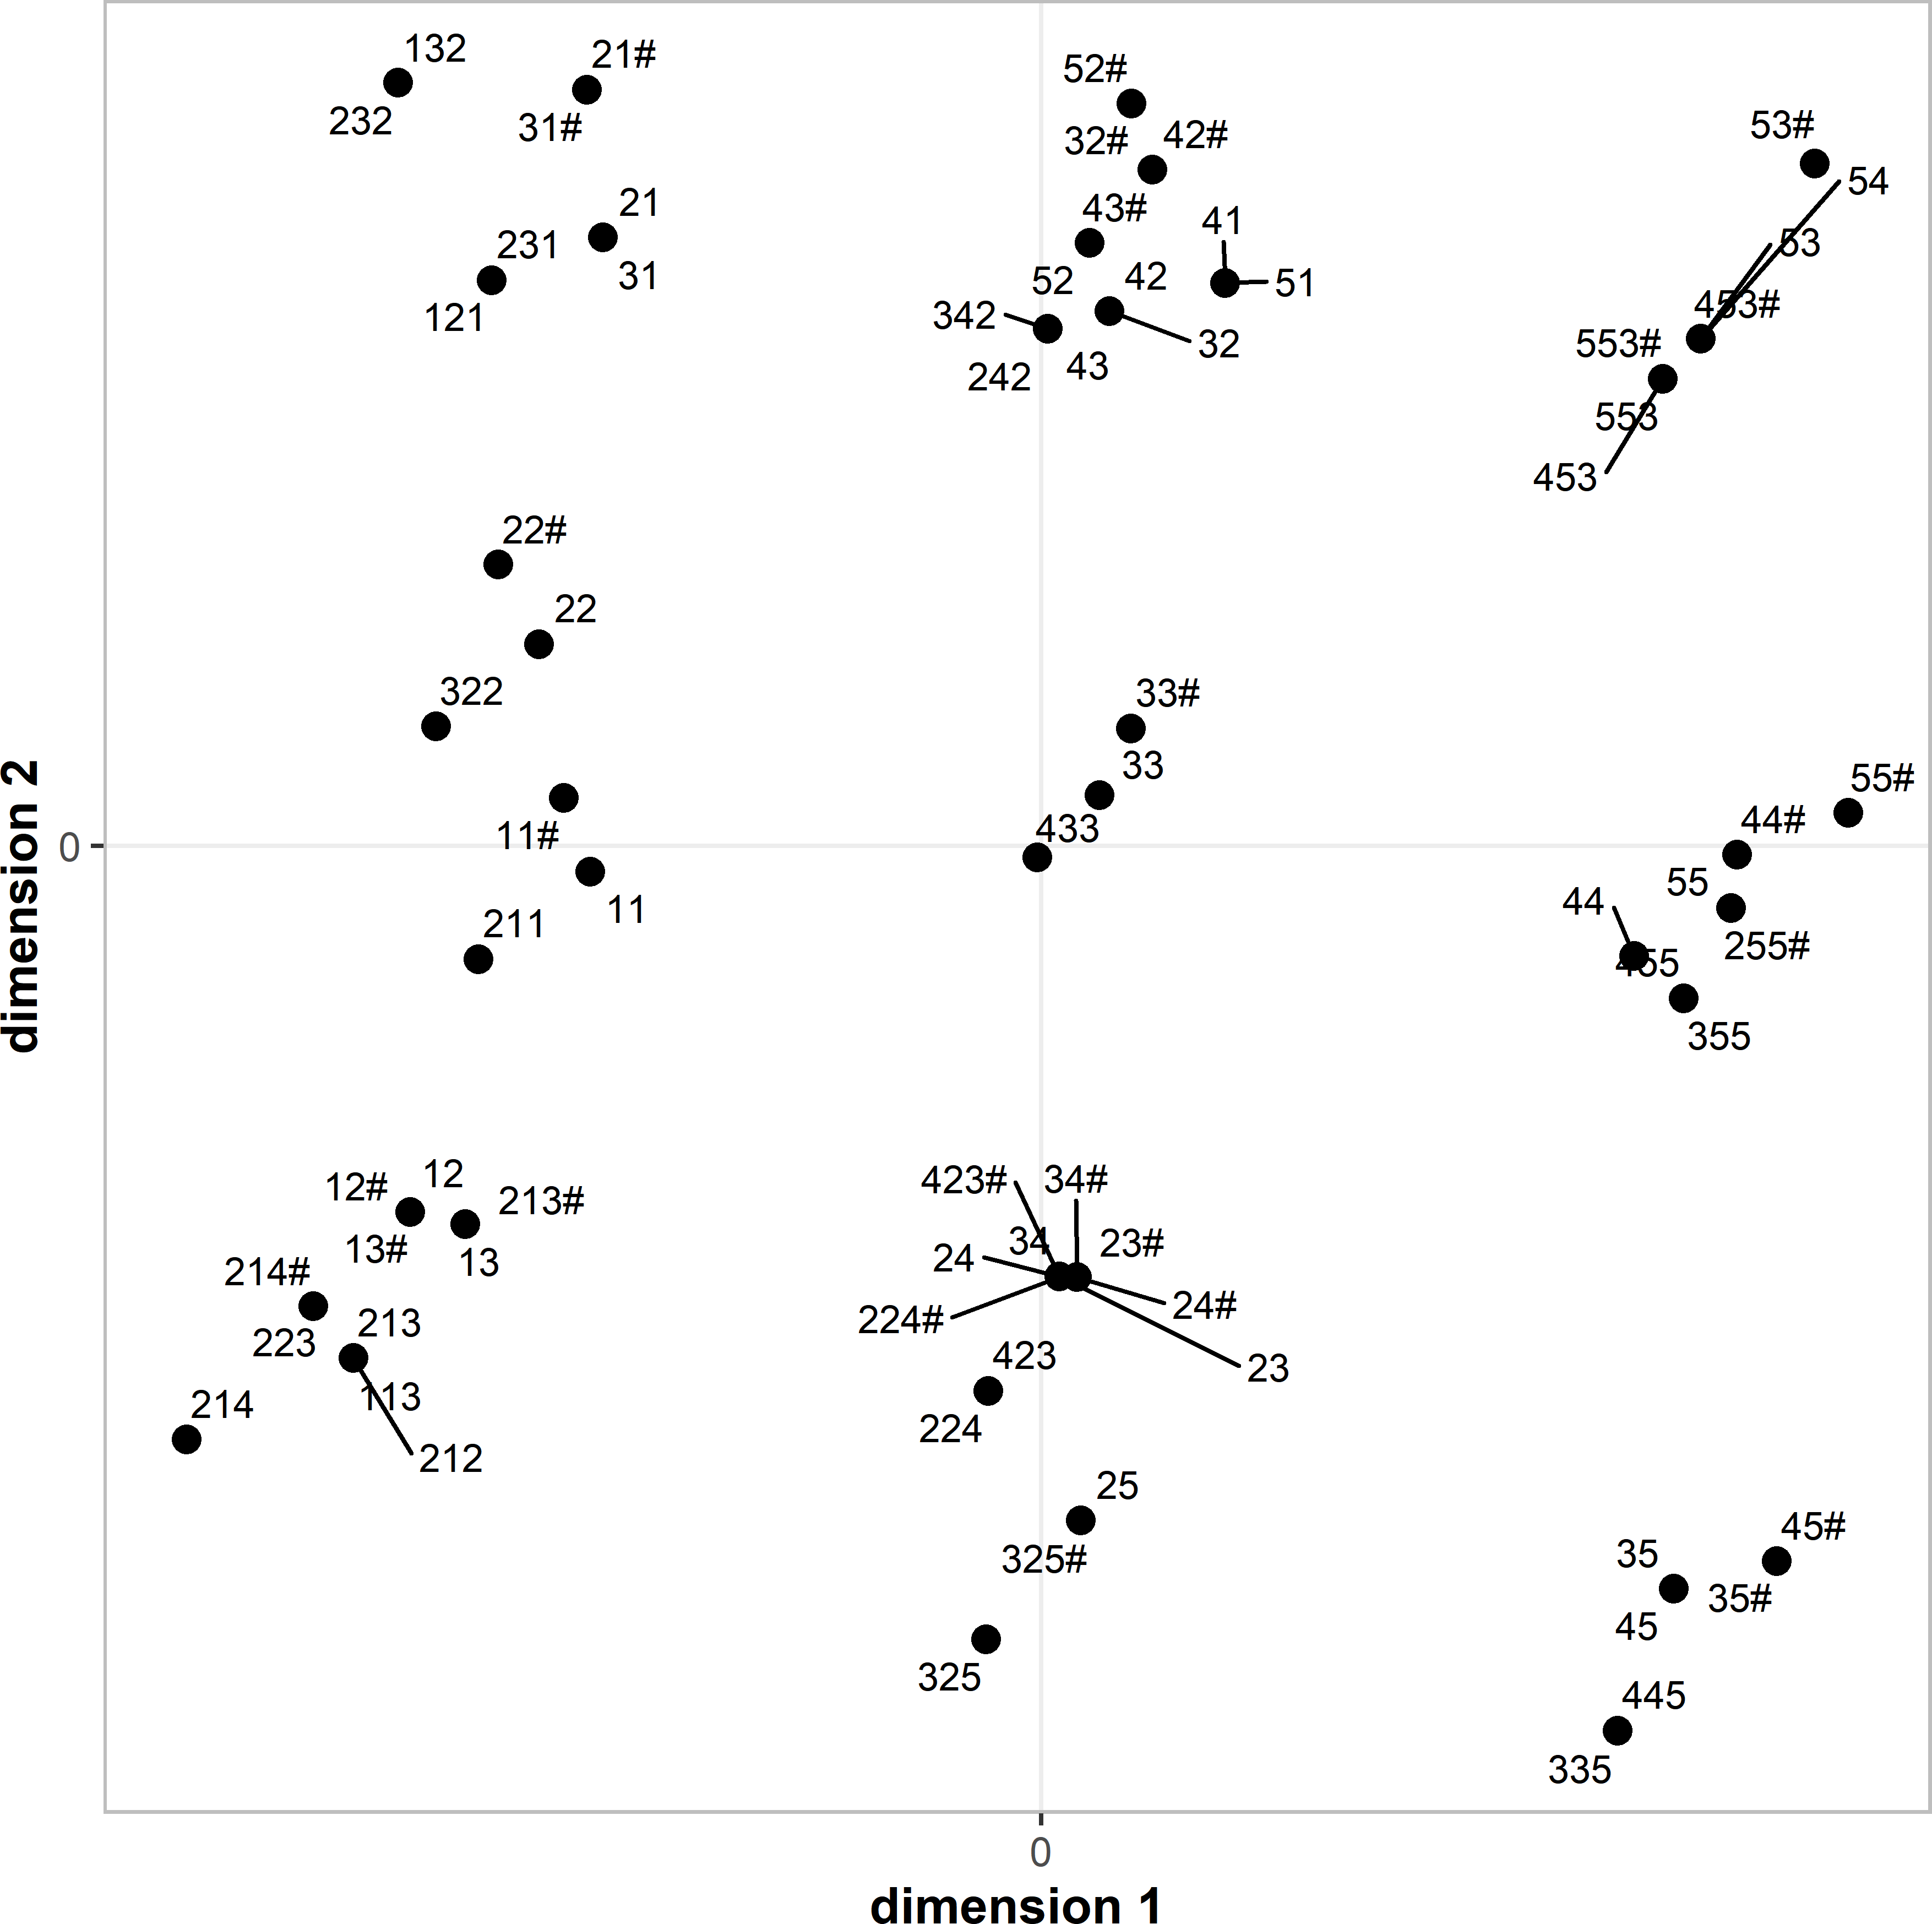
\includegraphics[width=\textwidth]{sung-img007.png}
\caption{MDS plot for GH-T, r\textsuperscript{2} = 0.74}
\label{fig:sung:7}
\end{figure}

\citet{GandourHarshman1978} and \citet{Gandour1983} have consistently found that cross-linguistically, the two major perceptual dimensions in tones are average pitch and direction. The first two dimensions extracted from the MDS plots are summarized in \tabref{tab:sung:8}.

\vfill
\begin{table}[H]
\begin{tabularx}{\textwidth}{Xrr}
\lsptoprule
{Method} & {Dimension 1} & {Dimension 2}\\\midrule
\citet{GandourHarshman1978}, \citet{Gandour1983} & Average Pitch & Direction\\
Binary & Uninterpretable & Uninterpretable\\
Tone-to-string & Uninterpretable* & Uninterpretable*\\
OCO & Direction & Average Pitch\\
GH-T & Average Pitch & Direction\\
\lspbottomrule
\end{tabularx}
\caption{Interpretation of the first two dimensions in the MDS plots of each tone distance measure}
\label{tab:sung:8}
\end{table}
\vfill\pagebreak

Firstly, the MDS plots for the Binary method requires some explanations. \figref{fig:sung:4a} is plotted using the Classical MDS and \figref{fig:sung:4b} is plotted using Sammon’s Mapping. Classical MDS was first used because the distance data is ratio data (\citealt{BorgGroenen2005}: 23). However, we realized that the plot in \figref{fig:sung:4a} does not make much sense. There is a central cluster, with some tones in isolation, e.g. 42, 211, but the nature of the binary method should not yield any clusters (as shown in the middle of \figref{fig:sung:4a}), since all the tones are equally distant to each other. Since the relationship between the tones may not be 2-dimensional\footnote{However, LED-A did not provide the explained variance value, nor did Gabmap work with this type of distance matrix (everything has a distance of 1 except itself).}, this gave us the motivation to go for Sammon’s Mapping (\figref{fig:sung:4b}), as it is designed for non-linear data structure \citep{Sammon1969}, and the plot resembles the distance matrix that we produced, where each tone is only similar (distance = 0) to itself, and all the tones are dispersed.

Summarized in \tabref{tab:sung:8}, the first two dimensions of the Binary method (\figref{fig:sung:4b}) are uninterpretable. One of the reasons could be because the distance matrix was constructed based on how all the tones in the data are equally different (except itself), so that the MDS plot is just displaying all the tones without taking into account the room of gradual similarity between the tones in the data (which the Binary method did not measure at all). The MDS plot for Tone-to-string (\figref{fig:sung:5}) is also uninterpretable if we only focus on Dimensions 1 and 2.\footnote{In terms of the procedures, it is possible to extract dimensions beyond dimension 2. With three and four dimensions, the cumulative explained variances are 0.40 and 0.55 respectively. However, if the first dimension, which has the highest variance explained for the distance matrix, is not even interpretable, the higher dimensions, which have lower explained variances, probably will not yield more insights and validity to the method.} However, tones in \figref{fig:sung:5} are clustered together loosely by the pitch level that the tone ends in. This suggests the plot is a product of the operations and calculations on the string (of the tone letters), instead of the actual linguistic component of the tones. The OCO representation (\figref{fig:sung:6}) shows a clearer picture than the previous two methods. For Dimension 1, we can see that on the right of the y-axis, the tone contours tend to be falling (e.g. 32, 52 and 53), and on the left, the contours tend to be rising (e.g. 12, 25, 45). For the level tones, they somewhat sit near the middle (y-axis). For Dimension 2, we can see that the tones above the x-axis tend to have a low onset, and their average pitches are mostly below 2.5. On the other hand, the tones under the x-axis are the opposite. Lastly, the GH-T plot (\figref{fig:sung:7}) shows nine clear clusters across the plot. The first dimension also shows average pitch differences; if we look at the dots around the x-axis, we can easily identify that the low-level tones are clustered on the left, mid-level tones are clustered in the middle, and high-level tones on the right. The second dimension also quite clearly suggests direction. If we focus on the dots around the y-axis, we will discover that the clusters of tones go from falling to level to rising, starting from the top.

\subsection{Local incoherence}
\label{sec:sung:5.2}
Local Incoherence shows how different/ similar a dialect is to its nearest dialects (see \sectref{sec:sung:4.2}). The local incoherence scores of each of the methods are calculated using \textit{Gabmap} \citep{Nerbonne2011, Leinonen2016}. The results are shown in \tabref{tab:sung:9}.


\begin{table}
\begin{tabular}{lr}
\lsptoprule
{Distance measure} & {Local incoherence}\\
\midrule
OCO & 4.51\\
Tone-to-string & 3.63\\
Binary comparison & 3.74\\
GH-T & 4.36\\
Segments (classic Levenshtein) & 2.10\\
\lspbottomrule
\end{tabular}
\caption{Local Incoherence scores for each tone distance measure and segments. Lower values represent better fit to the Fundamental Dialectological Postulate.}
\label{tab:sung:9}
\end{table}

The optimal score of Local Incoherence is 0, and from \tabref{tab:sung:9}, we see that none of the tone distance measures gets closer to 0 than the segmental level. Within the tone distance measures, Tone-to-string gets the lowest score, although it is not much lower than Binary comparison. OCO appears to be the method that produces the highest local incoherence, compared to the more linguistically naïve methods, while GH-T sits in between Binary and OCO.

In general, all tone distance measures have higher local incoherence than segments. This suggests two possibilities. The first possibility is that none of these measures are currently good enough to capture geographical variation of tones. The second possibility is that tones behave differently from segments, i.e. tones do not follow the \textit{Fundamental Dialectological Postulate}. An additional contribution to a high local incoherence might come from similar varieties (Guangfu and Yongxun dialects, see Appendix Map 1) distributed in such a long distance apart, with the Yongxun dialects surrounded by dissimilar dialects in the west \citep{Sung2023}. In order to explore these possibilities further, the tone distance measure should be refined first, so that inherent problems of each measure can be eliminated from the investigation, and a smaller region (e.g. Guangdong) can be investigated, in order to avoid the irregularity of distance introduced by the Yongxun dialects in Guangxi.

\subsection{Adjusted Rand Index (ARI)}
\label{sec:sung:5.3}
The cluster solutions of each of the tone distance measures (calculated with \textit{Gabmap} \citep{Nerbonne2011, Leinonen2016}) are compared to the traditional taxonomy from the \textit{Language Atlas of China} as well as the segmental distances (also calculated with classical Levenshtein distance with \textit{Gabmap}\footnote{Another segmental distance measure, PMI Levenshtein (\citealt{WielingEtAl2011}), which automatically infers segmental distances from 0 to 1 (instead of purely 0 or 1 in classical Levenshtein) based on the co-occurrence of segments, is not used. This is because the segmental distances inferred do not resemble to their acoustic distances (e.g. vowels do not show height and backness), unlike other languages tested using the same method in \citet{WielingEtAl2011}.}) by using the ARI. ARIs indicate how much cluster solutions overlap with the Reference Classification (see \sectref{sec:sung:3.2}). Results are shown in \tabref{tab:sung:10}.



%
\begin{table}
% \footnotesize
% \begin{tabular}{lrrrrrr}
% \lsptoprule
%  & LAC & Segments & Binary & Tone-to-string & OCO & GH-T\\
%  \midrule
%  LAC & 1 & 0.43 & 0.07 & 0.18 & 0.20 & 0.13\\
%  Segments & 0.43 & 1 & 0.13 & 0.17 & 0.19 & 0.14\\
%  Binary & 0.07 & 0.13 & 1 & 0.42 & 0.32 & 0.34\\
%  Tone-to-string & 0.18 & 0.17 & 0.42 & 1 & 0.44 & 0.42\\
%  OCO & 0.20 & 0.19 & 0.32 & 0.44 & 1 & 0.50\\
%  GH-T & 0.13 & 0.14 & 0.34 & 0.42 & 0.50 & 1\\
% \lspbottomrule
% \end{tabular}

\begin{tabular}{lS[table-format=1.2,round-mode=places,round-precision=2] S[table-format=1.2,round-mode=places,round-precision=2] S[table-format=1.2,round-mode=places,round-precision=2] S[table-format=1.2,round-mode=places,round-precision=2] S[table-format=1.2,round-mode=places,round-precision=2] S[table-format=1.2,round-mode=places,round-precision=2] }
\lsptoprule
 & {LAC}& {Segments}& {Binary}& {Tone-to-string}& {OCO}& {GH-T}\\
\midrule
 LAC & 1 & 0.47397809 & 0.086816453 & 0.213968775 & 0.248830419 & 0.175446341\\
Segments & 0.47397809 & 1 & 0.128285354 & 0.170559653 & 0.191291009 & 0.136672274\\
Binary & 0.086816453 & 0.128285354 & 1 & 0.417229332 & 0.317176519 & 0.336109314\\
Tone-to-string & 0.213968775 & 0.170559653 & 0.417229332 & 1 & 0.437931329 & 0.424621696\\
OCO & 0.248830419 & 0.191291009 & 0.317176519 & 0.437931329 & 1 & 0.501917101\\
GH-T & 0.175446341 & 0.136672274 & 0.336109314 & 0.424621696 & 0.501917101 & 1\\
\lspbottomrule
\end{tabular}
\caption{ARI Similarity matrix between tone distance measures, traditional classification and segmental classification. Higher scores represent more overlap.}
\label{tab:sung:10}
\end{table}

The ARI score of 1 represents a complete overlap of cluster solutions between two classifications. In \tabref{tab:sung:10}, the highest ARI score belongs to the pair of OCO and GH-T. In fact, OCO, GH-T and the Tone-to-string method all share high resemblance in terms of the classifications they yield. In fact, they are even higher than the ARI between the traditional classification and the segmental classification.

When we set the Reference Classification to LAC, the closest classification to the traditional taxonomy is the classical Levenshtein segmental classification, with 0.47. In terms of tone classifications, OCO had a score of 0.25 followed by Tone-to-string with 0.21. Between the segmental classification and the tone distance calculation methods, OCO resembles segments the most, with an ARI score of 0.19, while Tone-to-string follows with an ARI of 0.17. Overall, the Binary method has the lowest ARI score with almost all classifications. Although OCO and Tone-to-string resemble the traditional and segmental classifications the most respectively, their ARI scores are rather low, suggesting rather dissimilar classifications.

\section{Discussion}
\label{sec:sung:6}
\subsection{Summary of results} \label{sec:sung:6.1}

The overall results are summarized in \tabref{tab:sung:11}.

\begin{table}
\footnotesize
\begin{tabularx}{\textwidth}{llllll}
\lsptoprule
{Method} & {Overlaps} & {Perceptual} & {Local} & \multicolumn{2}{c}{ARI}\\
& & dimensions & incoherence & & \\\cmidrule(lr){5-6}
& & & & Traditional & Segmental \\
& & & & classification & classification\\
\midrule
 Binary & \cellcolor[gray]{0.9}{None} & Uninterpretable & Intermediate & Lowest & Intermediate\\
%  \midrule
 Tone-to- & Intermediate & Uninterpretable & \cellcolor[gray]{0.9}{Lowest} & Intermediate & Intermediate\\
 string & & & & & \\
%  \midrule
 OCO & Highest & Resembles GH & Highest & \cellcolor[gray]{0.9}{Highest} & \cellcolor[gray]{0.9}{Highest}\\
%  \midrule
 GH-T & Intermediate & \cellcolor[gray]{0.9}{Identical to GH} & Intermediate & Intermediate & Lowest\\
\lspbottomrule
\end{tabularx}
\caption{Overall results of evaluation across 4 tone distance calculation methods}
\label{tab:sung:11}
\end{table}

\subsection{Which method to choose?}\label{sec:sung:6.2}

Each tone distance calculation method seems to do better than the others in one specific task.  OCO has shown the best result with respect to two evaluation measures, while others performed best in one task each. This does not automatically make OCO the go-to method for the dialect classification of tones, though. OCO suffers the most from the overlapping representations, whilst the Binary method could distinguish all tones. The Binary method, however, cannot differentiate similar vs. very distinct tones, which makes the whole distance calculation rather arbitrary. For this reason, the Binary method is not suggested to be used in dialectometry.

In terms of perceptual dimensions, OCO shows some resemblance to \citegen{GandourHarshman1978}'s findings, but the relative importance of the dimensions is not in the right order, as reflected in the MDS plot (see \tabref{tab:sung:6}). This aspect, however, could be fixed, so OCO has some potentials in this sense. 

Looking at local incoherence, the best performing method is Tone-to-string, but like the Binary method, this method is also linguistically naïve. In addition, it’s first two dimensions on the MDS are uninterpretable, hence this method is also not recommended in dialectometry. However, readers should be reminded that local incoherence should be taken as a grain of salt here, as mentioned in \sectref{sec:sung:5.2}: The possibility that tones do not behave like segments and the dialect islands (Yongxun dialects) in the Guangxi province surrounded by dissimilar dialects both might contribute to the higher local incoherence. 

As suggested in \sectref{sec:sung:5.3} and based on the observation that there is low resemblance between the traditional, segmental and tonal (OCO, GH-T) classifications, there is a possibility that the nature of tonal variation is different from segments. Therefore, we cannot simply use the ARI scores as a determining factor for choosing one tone distance calculation over another. OCO shares the highest ARI score with GH-T (and to some extent, the perceptual dimensions), which makes both methods valid to be used in dialectometry, given that some improvements are made (e.g. increase the distinction rate). However, there is one consideration which makes us favour one method over another – the ability to combine tonal and segmental analysis. The segmental analysis is done using Levenshtein Distance, as does the OCO representation. Ideally, the method for calculating tone distances is not limited to a tone-only analysis, but also a combined analysis with segments. This will not be possible with GH-T, since it requires a separate specification of tone features. For this reason, we argue that the OCO method should be chosen and further improved.

\subsection{Possible improvements}
\label{sec:sung:6.3}
The most fundamental problem OCO has is being unable to distinguish tones in the dataset (not even 50\%). The first thing we should do is to find a way to take duration into consideration, and secondly, modifying the three-level distinction into five, since having five levels seems to be the maximum used by any language \citep[20]{Yip2002}. Another issue which has been pointed out is that some tones, although they have different contours, are still yielding the same difference under OCO.\footnote{Thanks to J. Fruehwald for his comment at Methods in Dialectology XVII.} 

We illustrate this with two tone pairs, 53 vs. 31 and 12 vs. 31. The former pairs are Falling tones (with the same slope), only differing in pitch levels. The latter pair are Rising and Falling tones respectively, and they have different degrees of slope. Many linguists would agree that one tone should be more different from 31 than the other. If we use the OCO representation to calculate tone difference, we get the same distance for these two tones. This is illustrated in \figref{fig:sung:8}.

  
\begin{figure}
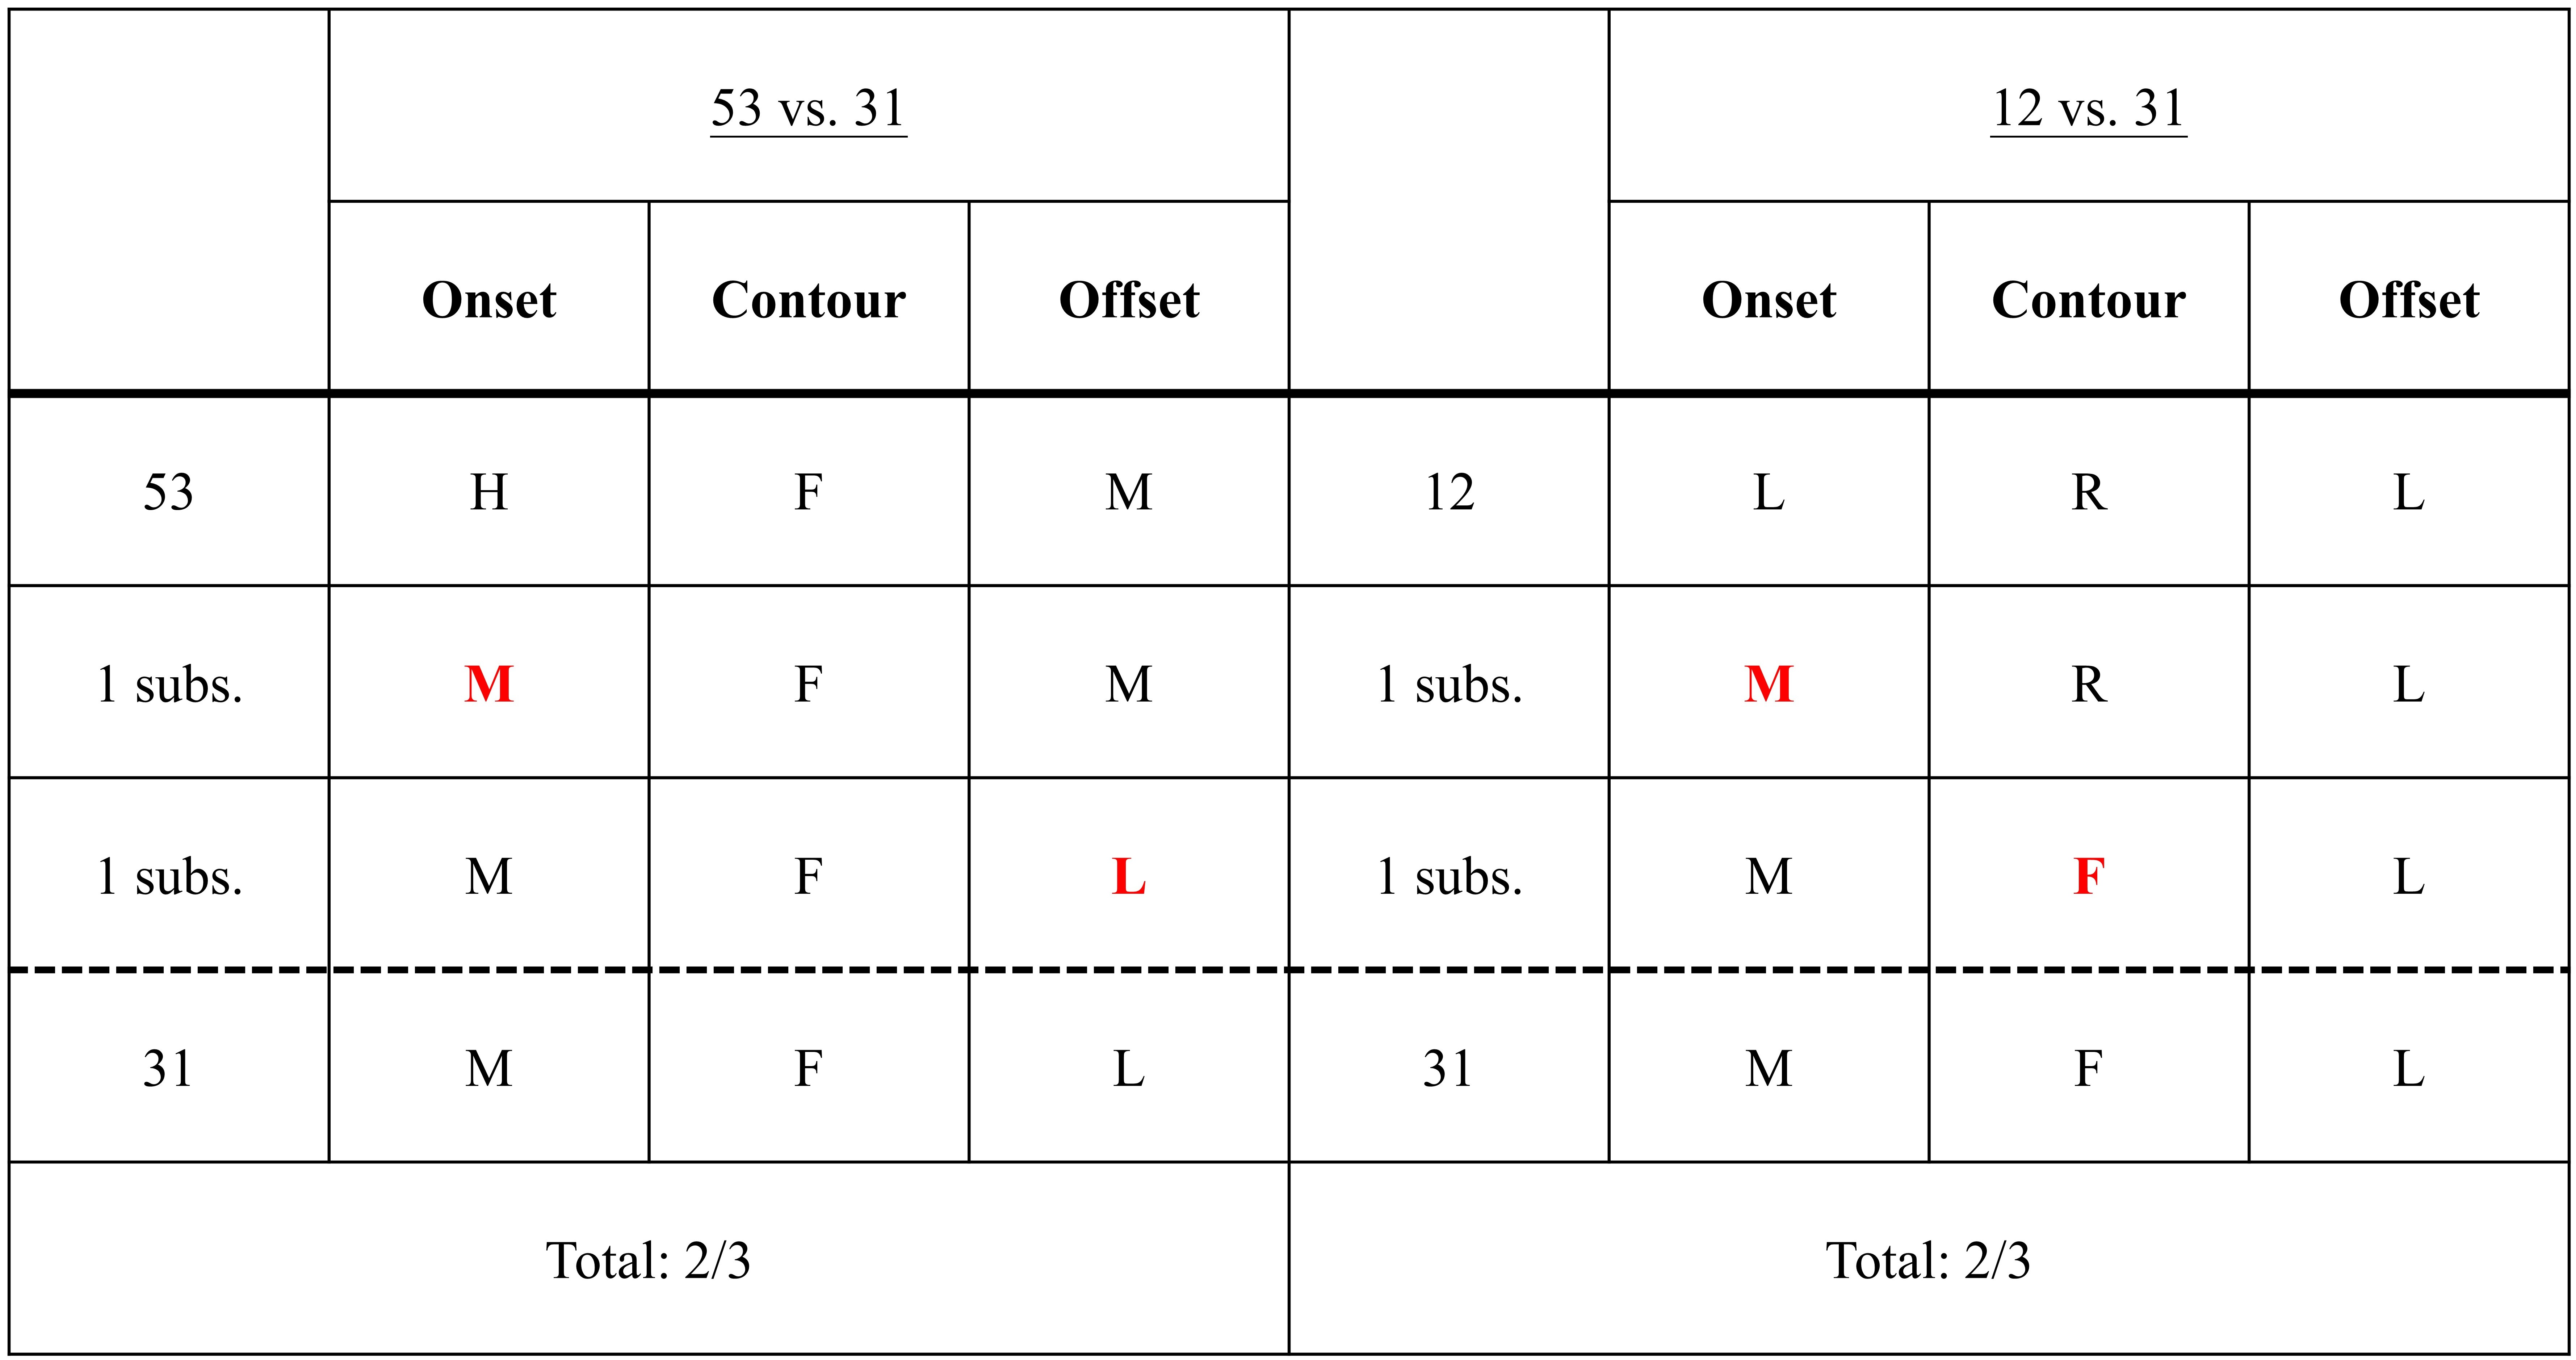
\includegraphics[width=\textwidth]{sung-img008.jpg}
\caption{Comparison of tones 53 and 12 with 31}
\label{fig:sung:8}
\end{figure}

As illustrated in \figref{fig:sung:8}, 53 vs. 31 only consisted of pitch differences, while 12 vs. 31 involves contour as well. However, using OCO representation this cannot be detected. In order to distinguish differences in these cases, perhaps weighting (onset, offset and/or contour) should be tested on each parameter\footnote{Reviewer 2 has suggested introducing \textit{steps} when dealing with substitution in the OCO representation. For example, if Onset or Offset has a High, then a substitution to Mid would be 1, but to Low would be 2. Similarly, for Contour, a substitution from Rising to Level would be 1, but to Falling would be 2.}. Alternatively, other features (based on perceptual cues, see \citealt{GandourHarshman1978}) shall be explored.

\subsection{Tonal variation in Yue and Pinghua}\label{sec:sung:6.4}

Lastly, we would like to make a remark on the patterns of tonal variation in the Yue and Pinghua-speaking so far. Although in general the ARI scores of the tone distances generated from each method and the segmental distances are relatively low, by visual inspection of the cluster maps (see Appendix), Tone-to-string, OCO and GH-T yield some clusters which resemble the segmental clusters, as well as the LAC a lot. For instance, Siyi dialects (consisting of 5 localities, Taishan, Kaiping, Enping, Xinhui and Doumen) can be identified, which align with both segmental and traditional classification. Another notable observation for the same methods is that we can see the East-most cluster (traditional Guangfu dialects) spread westward towards Guangxi. This pattern matches the segmental analysis, which can be explained by historical migration around 150 years ago (\citealt{Sousa2022}: 268). The other patterns are yet to be explained\footnote{Since the submission of this chapter, modifications of the OCO representation has been made and further analyses on tonal variation have been done. Please refer to \citet{sung2024exploring} for the follow up study.}.

To further understand the tonal variation of Yue and Pinghua (and any other tonal languages), therefore, we first need an improved way to calculate tone distances. That will allow us to find ways tones differ between dialects (e.g. is it gradual or abrupt?), to explore whether tones may behave differently from segments (as we have suggested in \sectref{sec:sung:4.2} with local incoherence) as well as the possibility of combining segments and tones in the same analysis.

\section{Conclusion}
\label{sec:sung:7}
Traditionally dialectology has focused on segments, and not much attention has been paid to tones, despite the wealth of data we have on tone languages, such as Sinitic languages. The limited research in exploring tone distance measures has only been tested on a small dataset. Hence, far from enough systematic comparison has been made on the existing methods for the purpose of dialect classification. This paper offers such systematic comparison, with a dataset which comprises of 104 dialects. Our results show that the OCO and GH-T representations make meaningful contributions to dialectometry, but they are not yet ready for the use in measuring tonal distances. We have suggested possible improvements and discussed the coherence problem between the tone distance calculation methods and tone changes.

Throughout the comparison, we repeatedly see that tones do not follow the same variation patterns as segments. Perhaps tonal variation really has a different nature in how it varies geographically. This is a rather unexplored area which awaits more research and improved methodology, and we hope that this paper is the first step in that direction.


\section*{Appendix}
\label{sec:sung:appendix}

\begin{figure}[H]
\rotatebox{90}{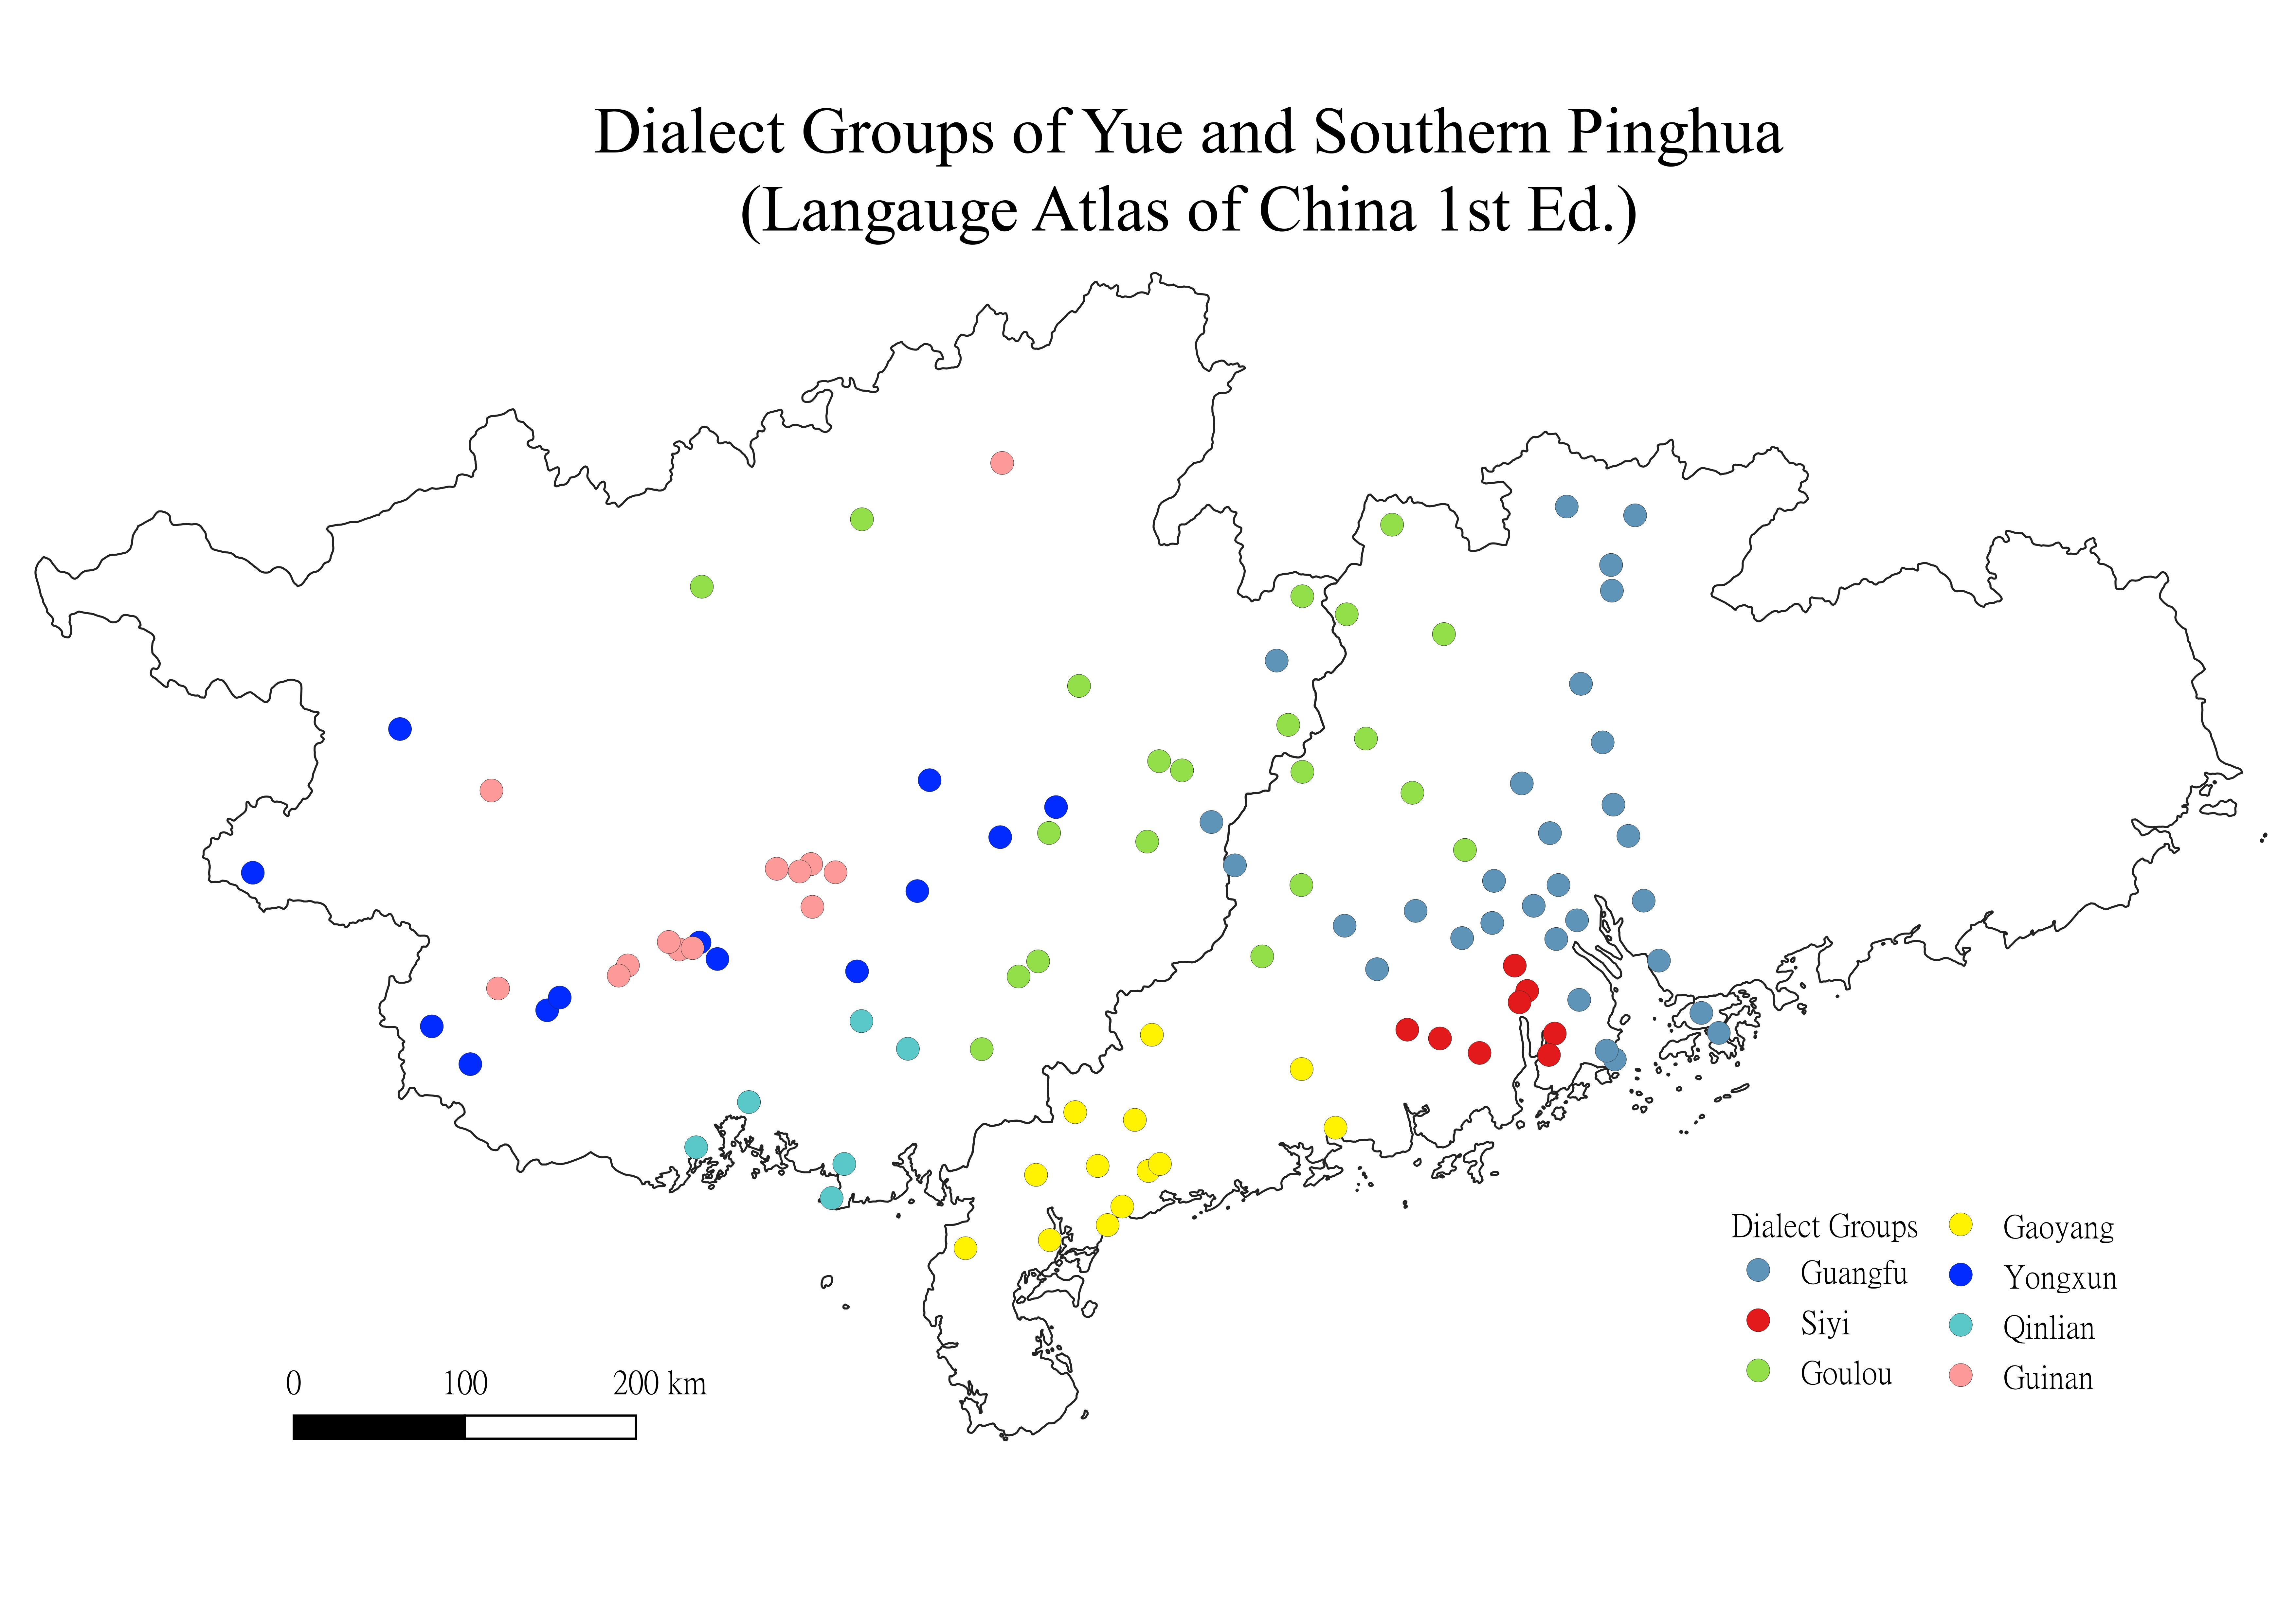
\includegraphics[width=16cm]{LAC_map_2025Feb.jpeg}}
\caption{\label{map:sung:1} Traditional classification of the dialects in the Yue-Pinghua data (based on Language Atlas of China)}
\end{figure}



\begin{sidewaysfigure}[H]
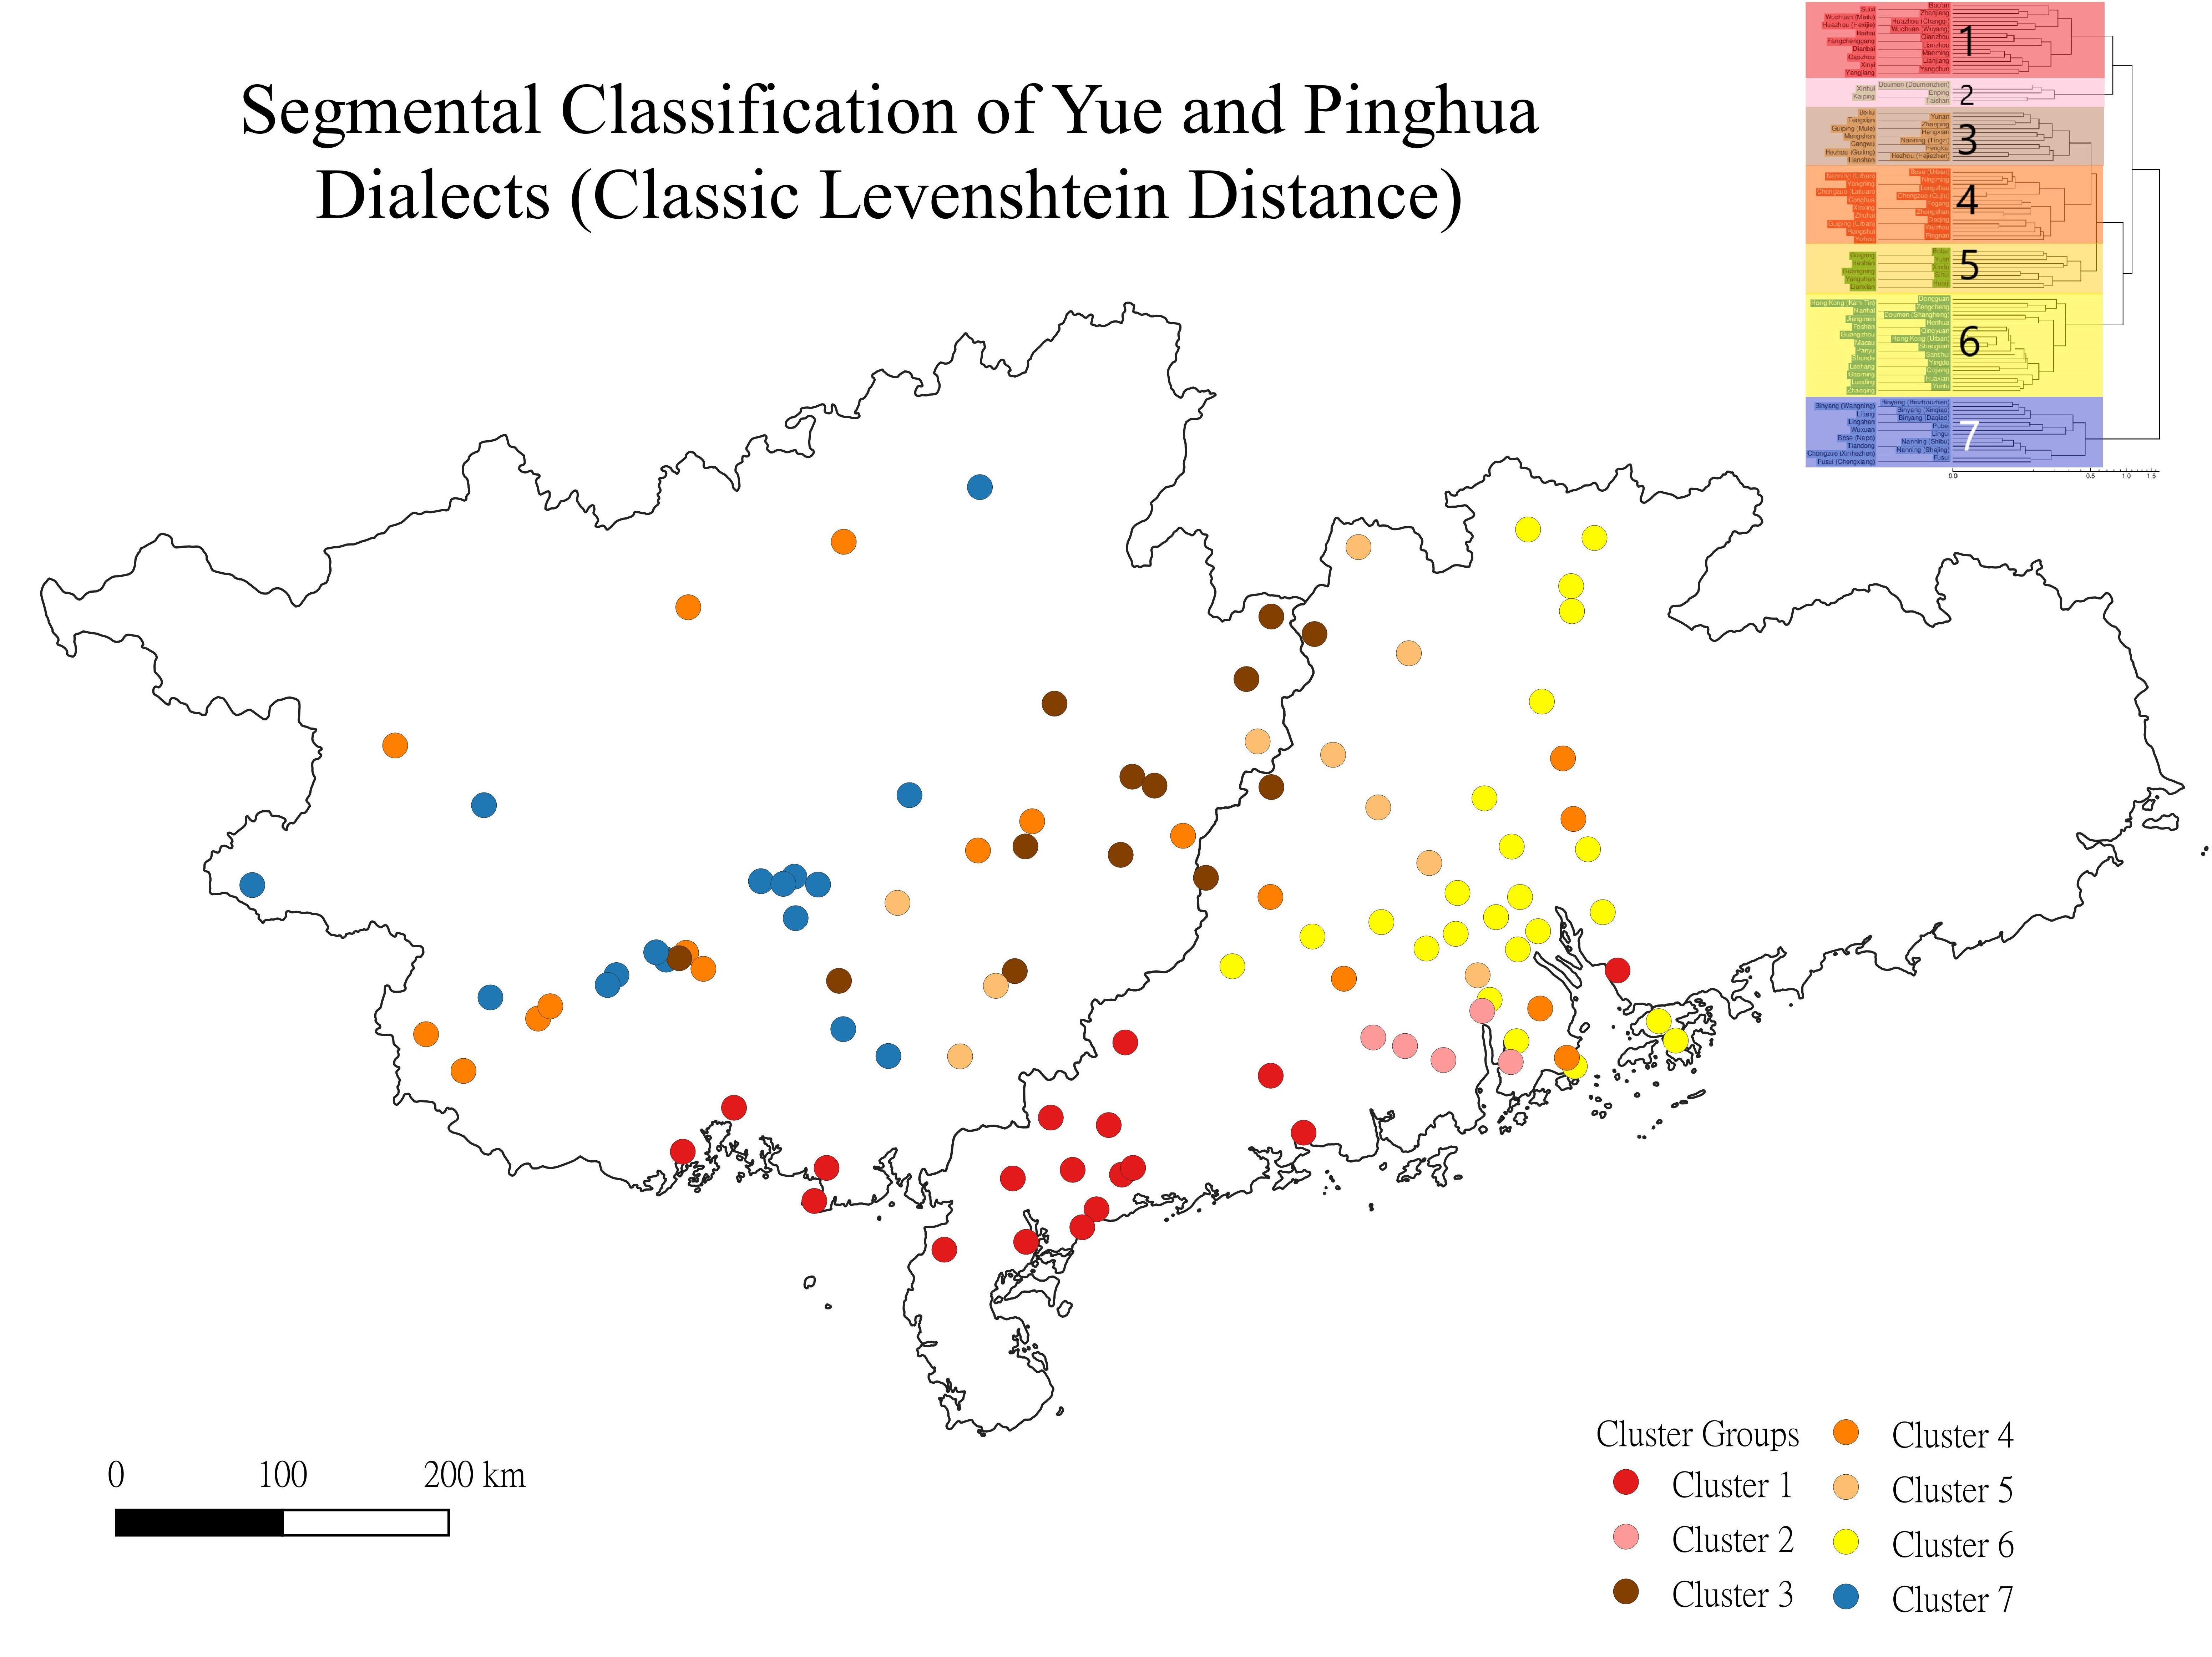
\includegraphics[width=16cm]{sung-map002_2.jpeg}
\caption{\label{map:sung:2} Cluster map (Ward’s method) of the segmental classification of the Yue-Pinghua data}
\end{sidewaysfigure}

 

\begin{sidewaysfigure}[H]
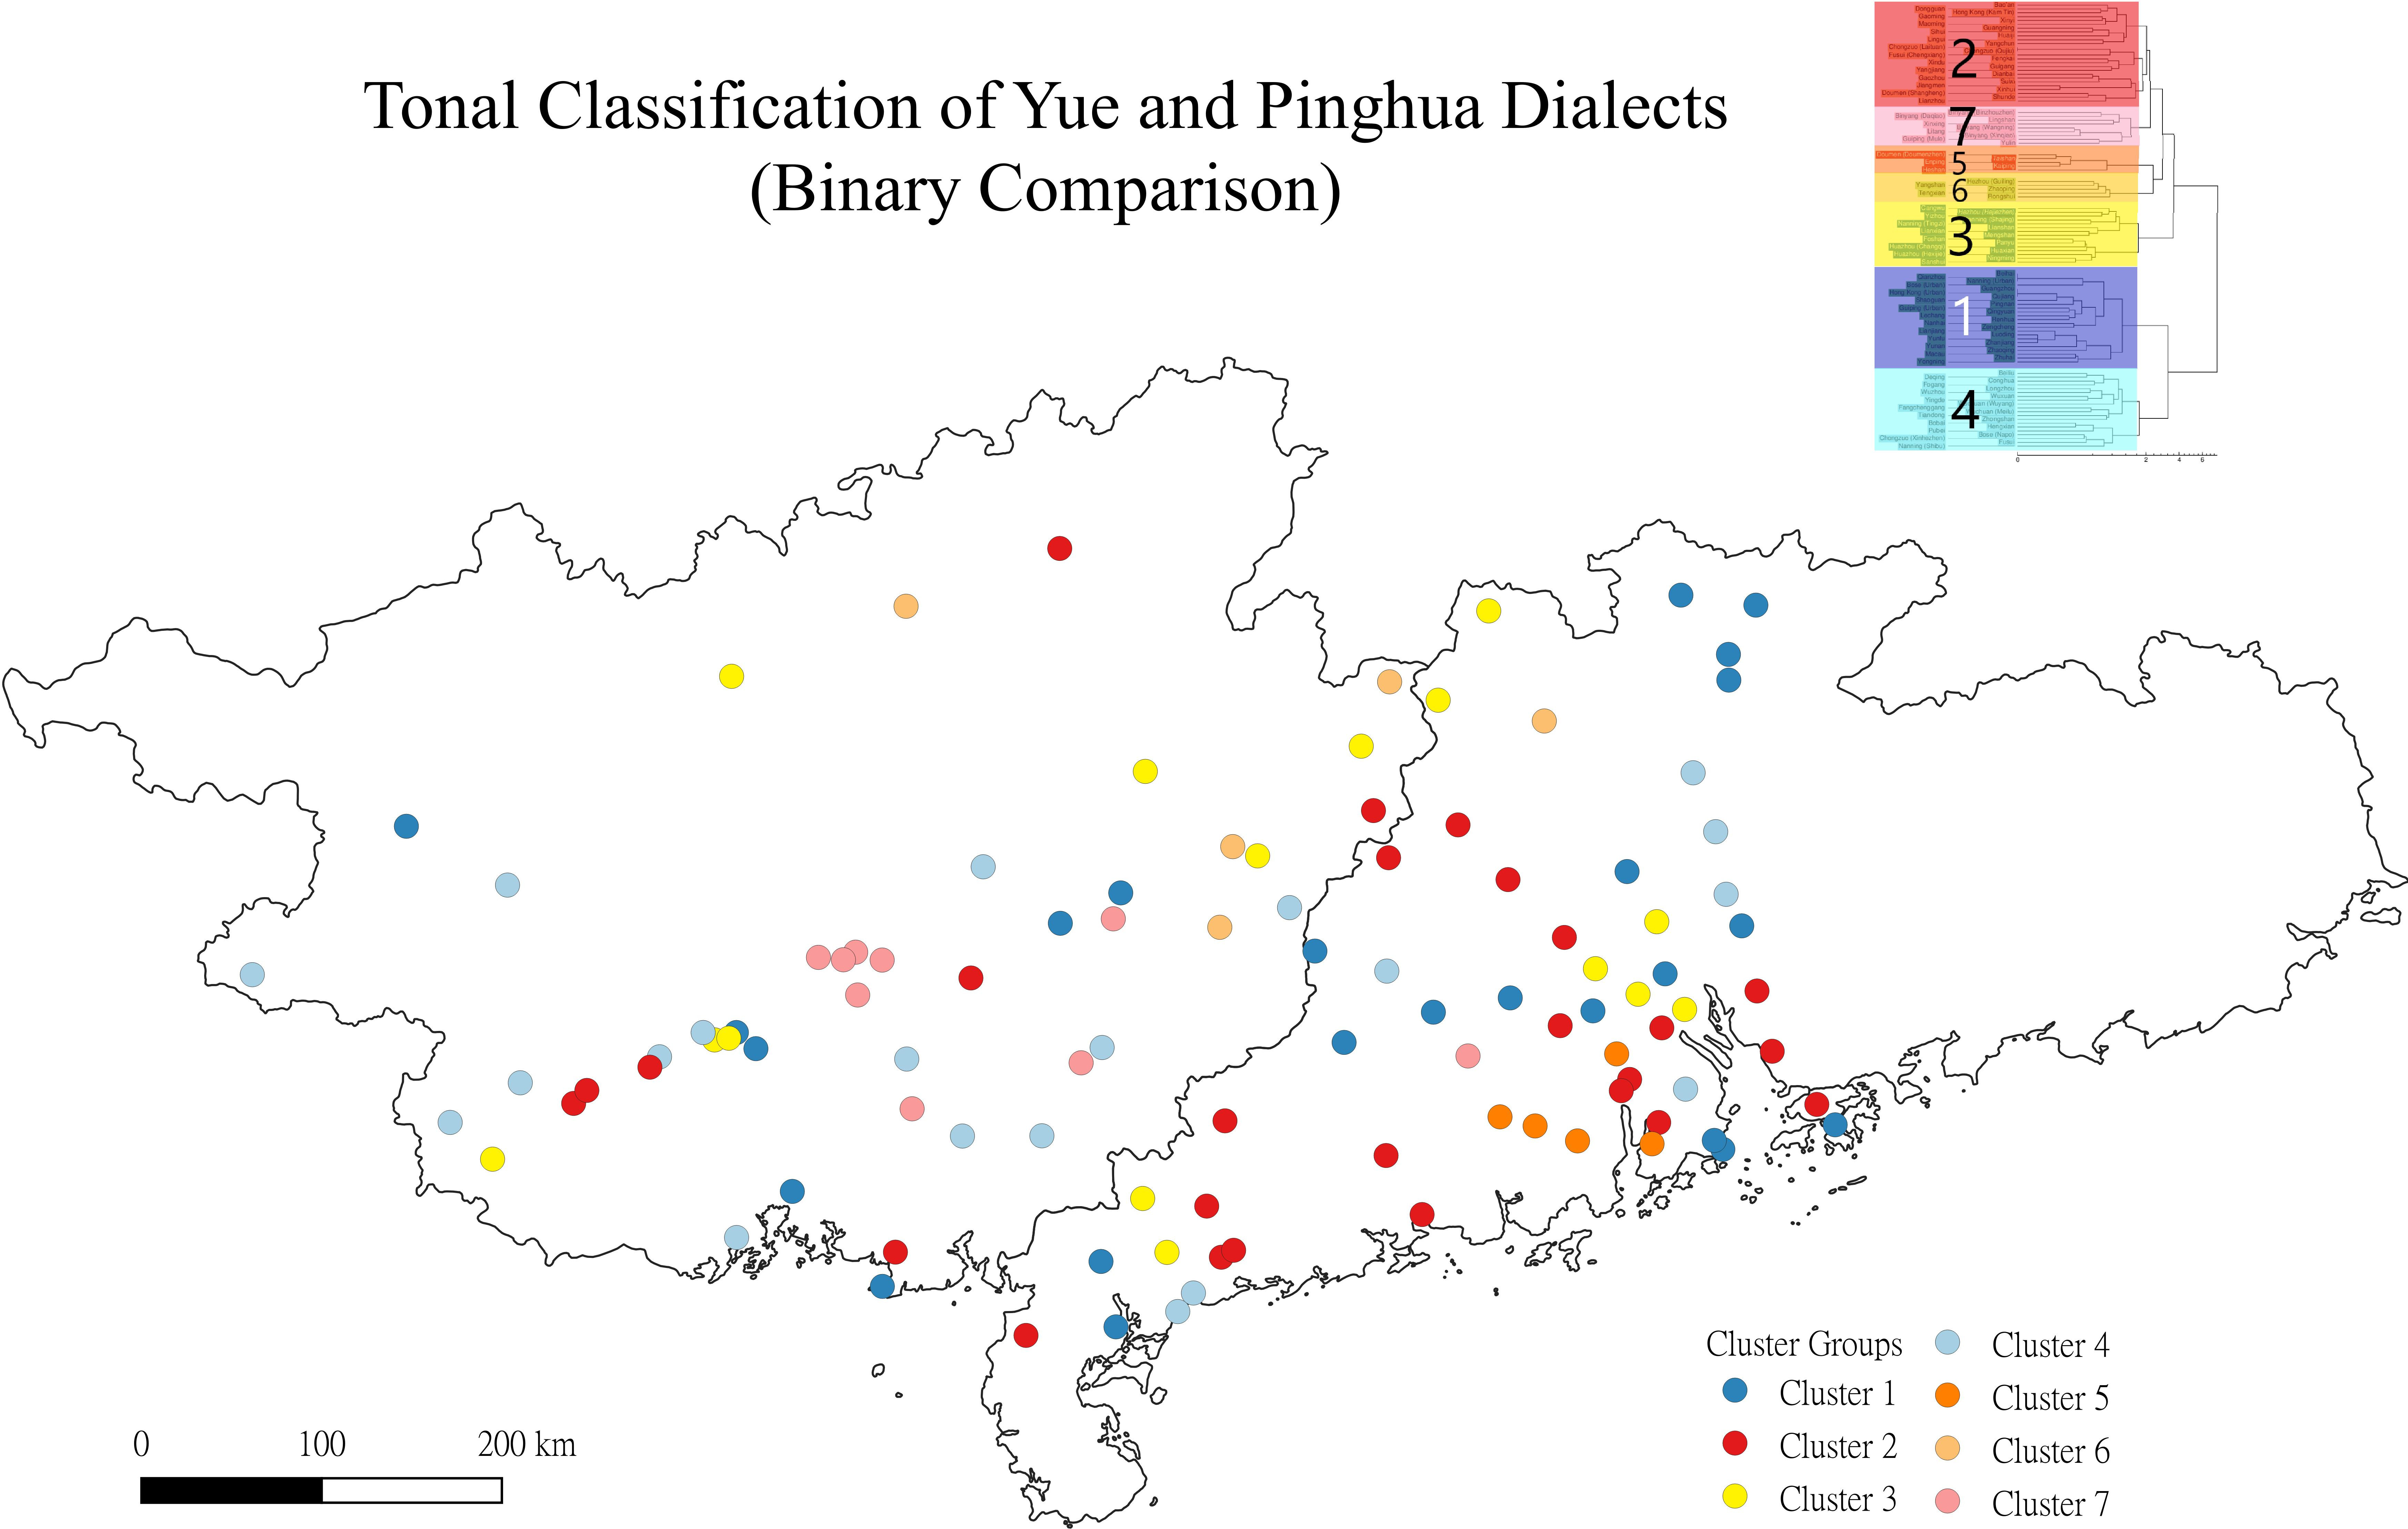
\includegraphics[width=16cm]{sung-map003.jpeg}
\caption{\label{map:sung:3bin} Cluster map (Ward’s method) of the tonal classification of the Yue-Pinghua data (Binary comparison)}
\end{sidewaysfigure}


\begin{sidewaysfigure}[H]
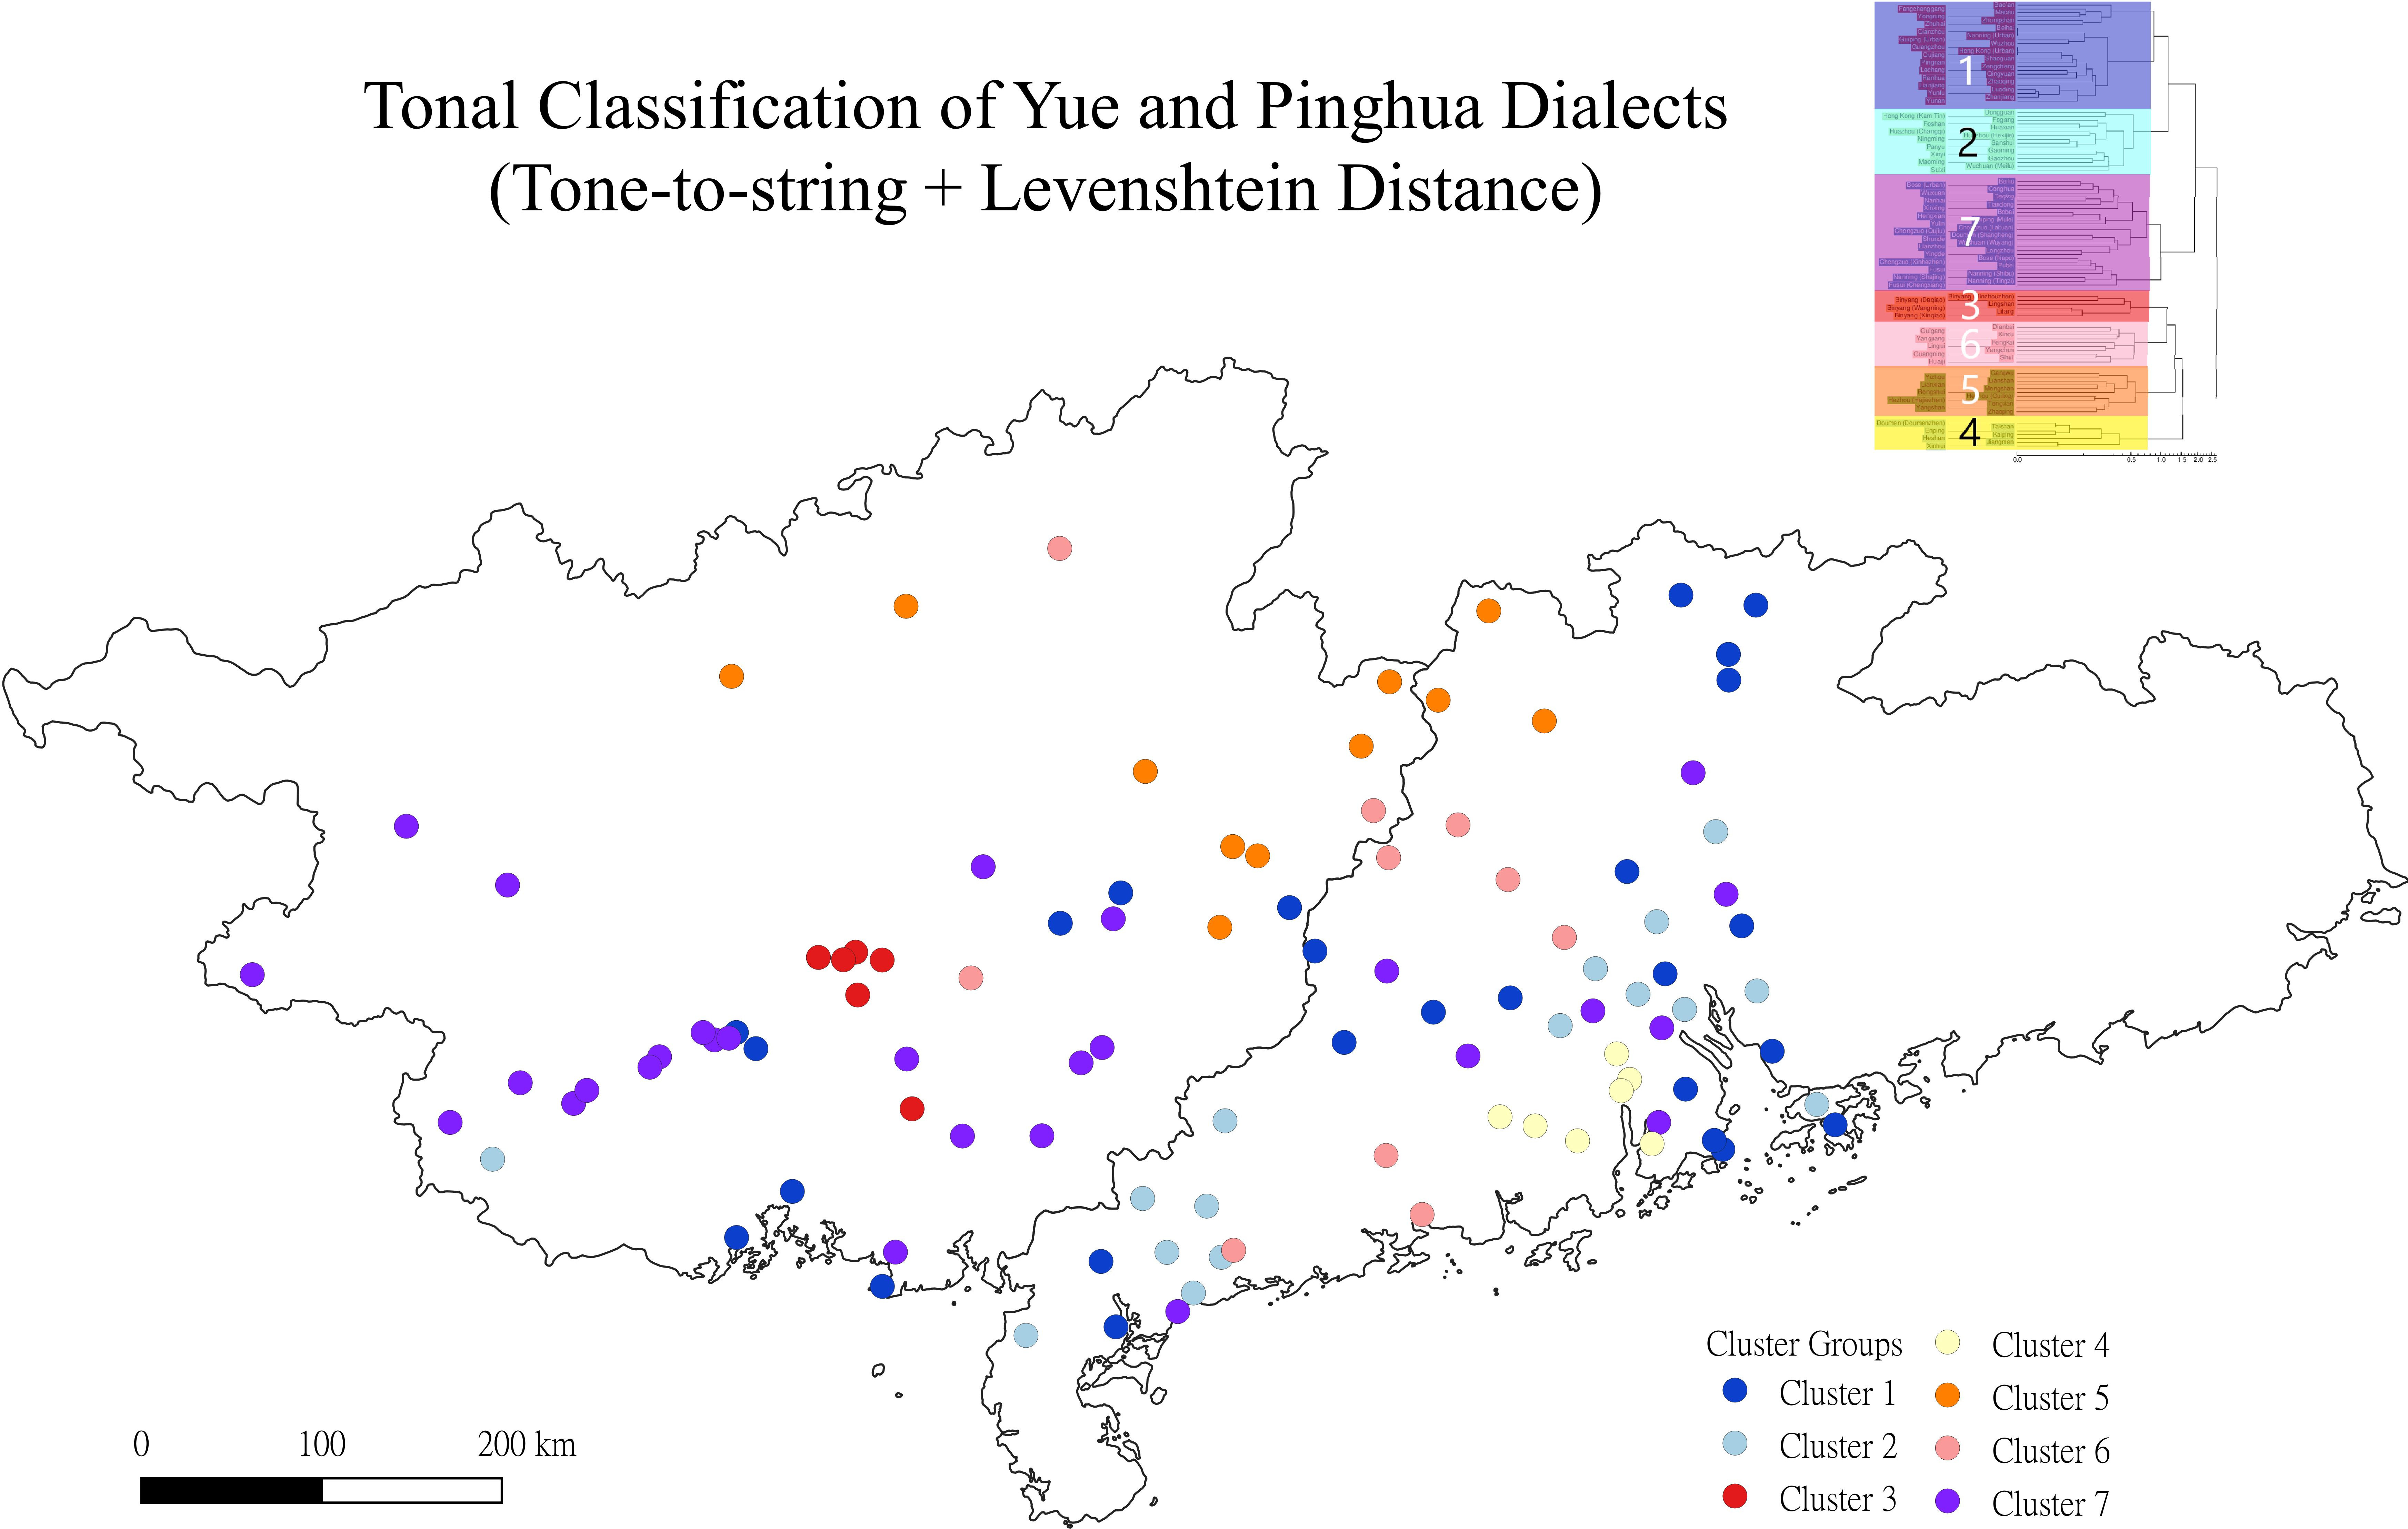
\includegraphics[width=16cm]{sung-map004.jpeg}
\caption{\label{map:sung:3lev}Cluster map (Ward’s method) of the tonal classification of the Yue-Pinghua data (Tone-to-string + Levenshtein distance)}
\end{sidewaysfigure}


\begin{sidewaysfigure}[H]
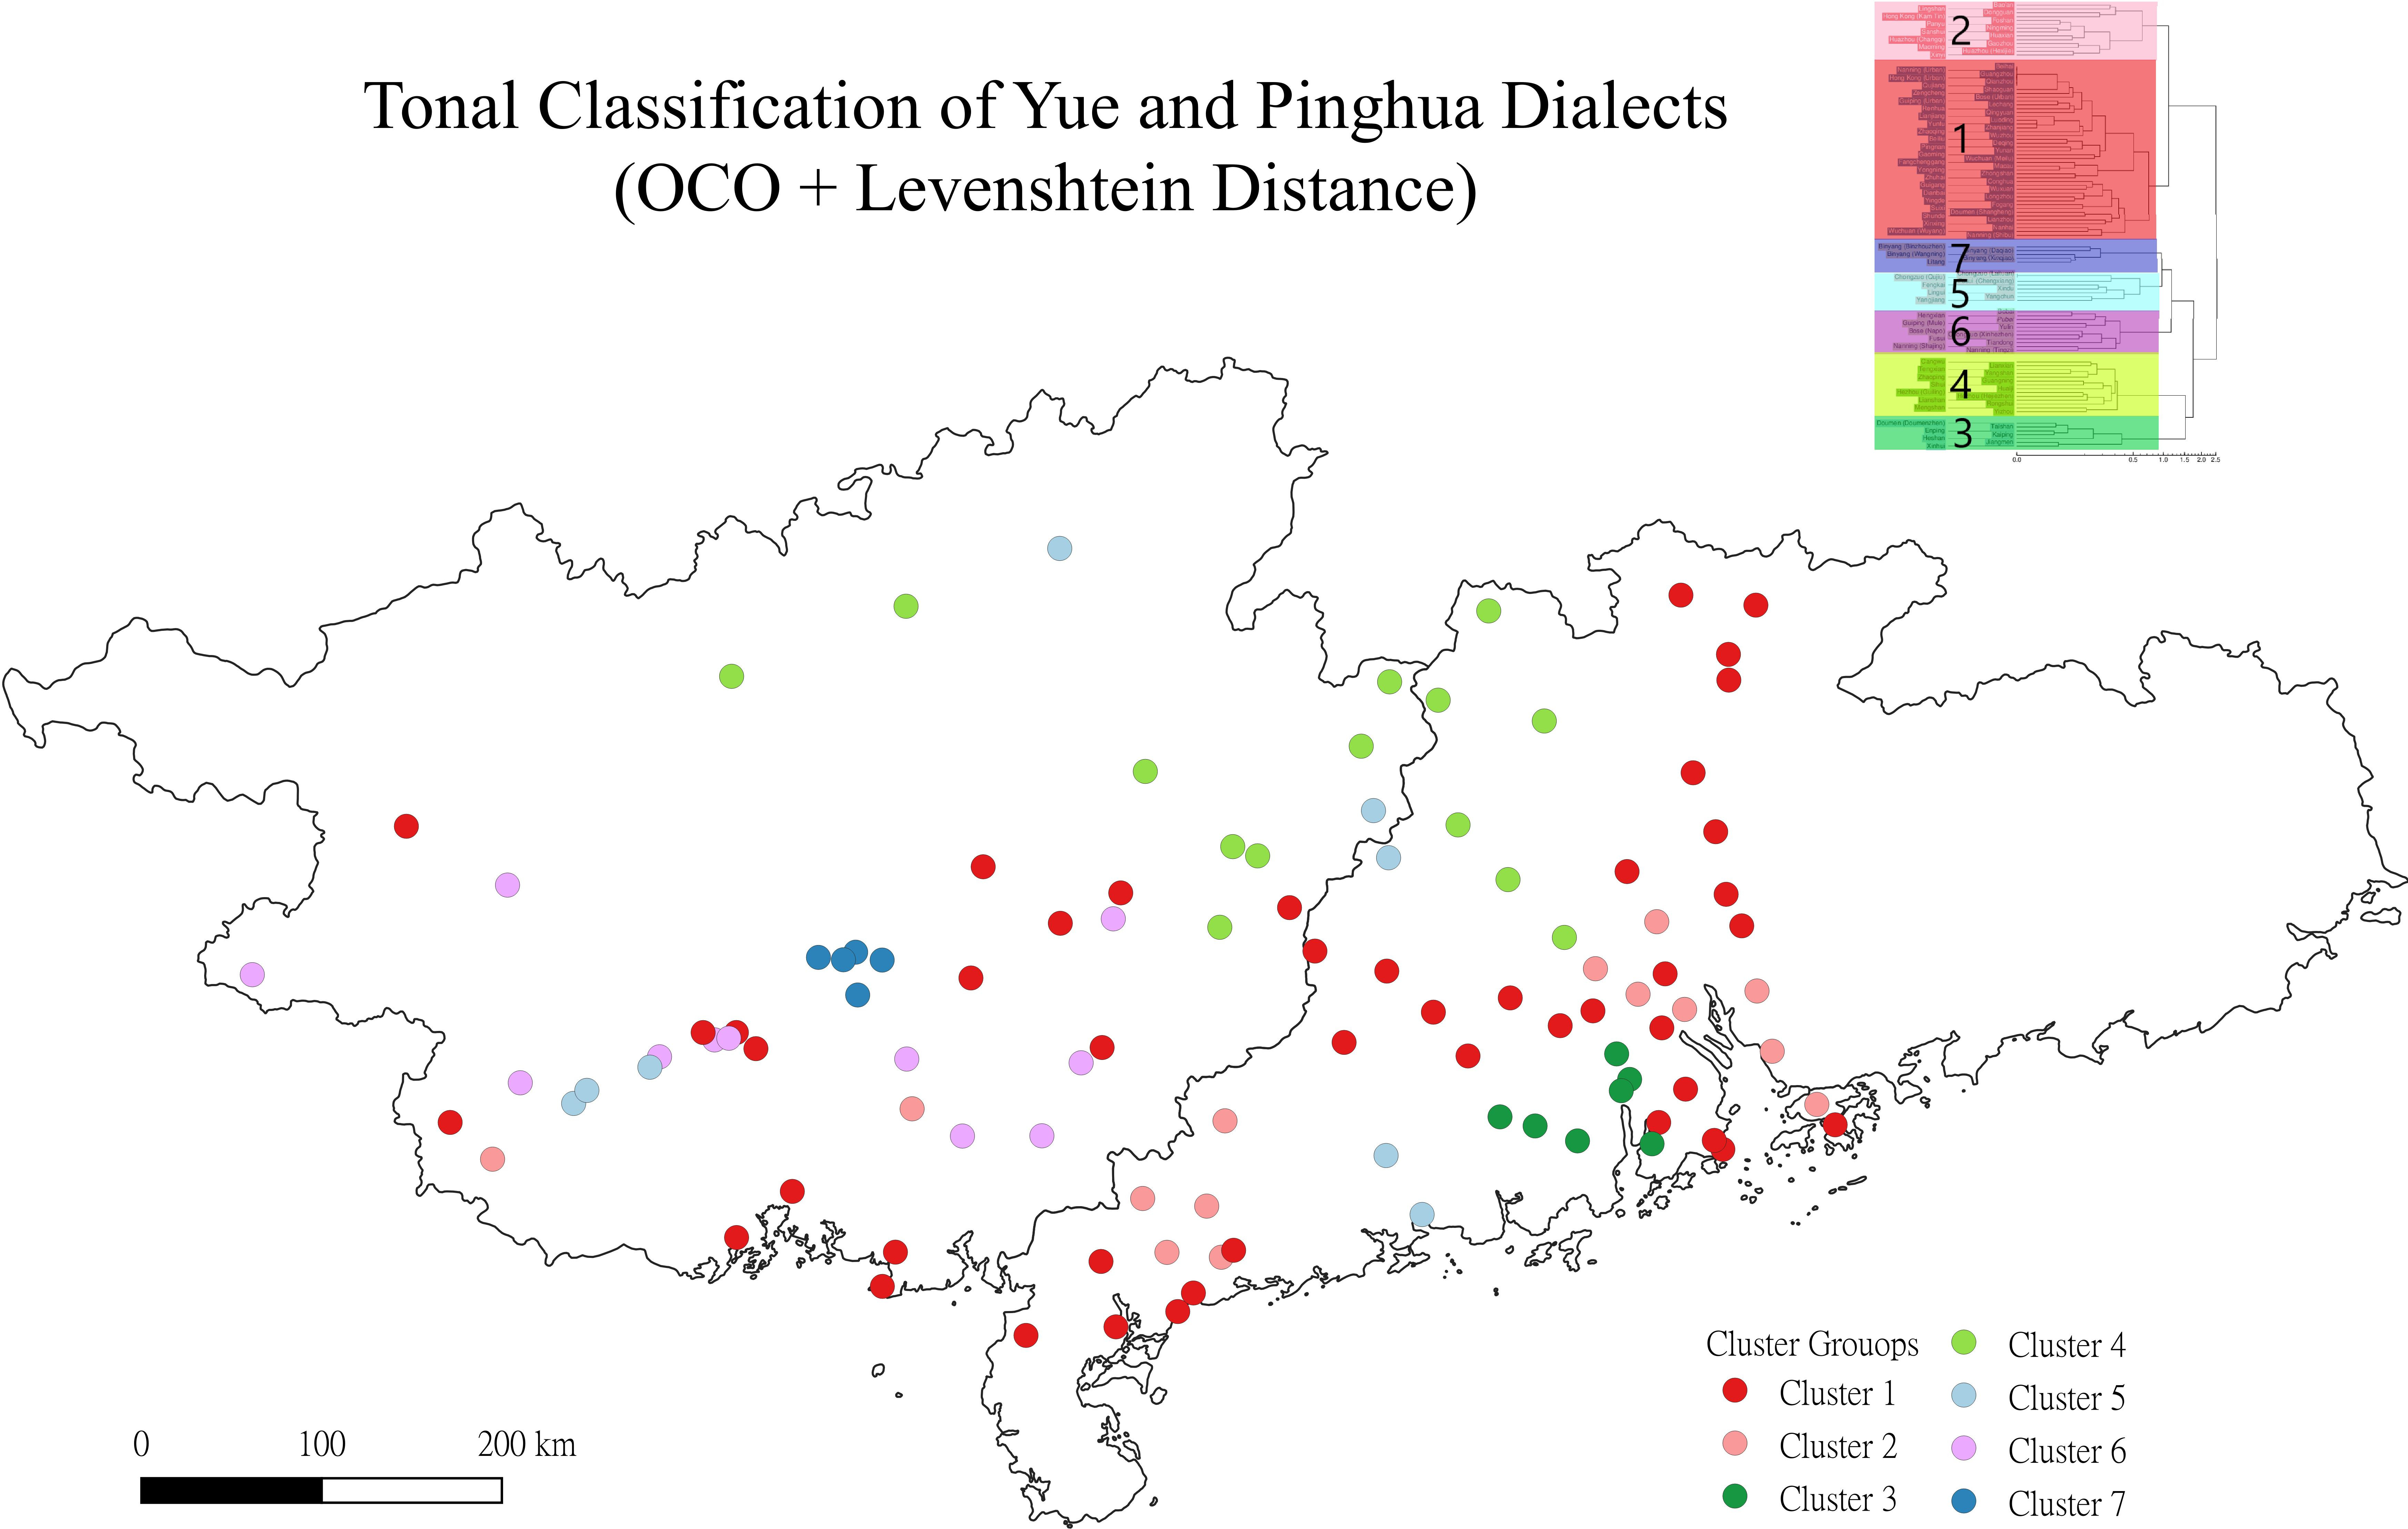
\includegraphics[width=16cm]{sung-map005.jpeg}
\caption{\label{map:sung:5} Cluster map (Ward’s method) of the tonal classification of the Yue-Pinghua data (OCO + Levenshtein distance)}
\end{sidewaysfigure}


\begin{sidewaysfigure}[H]
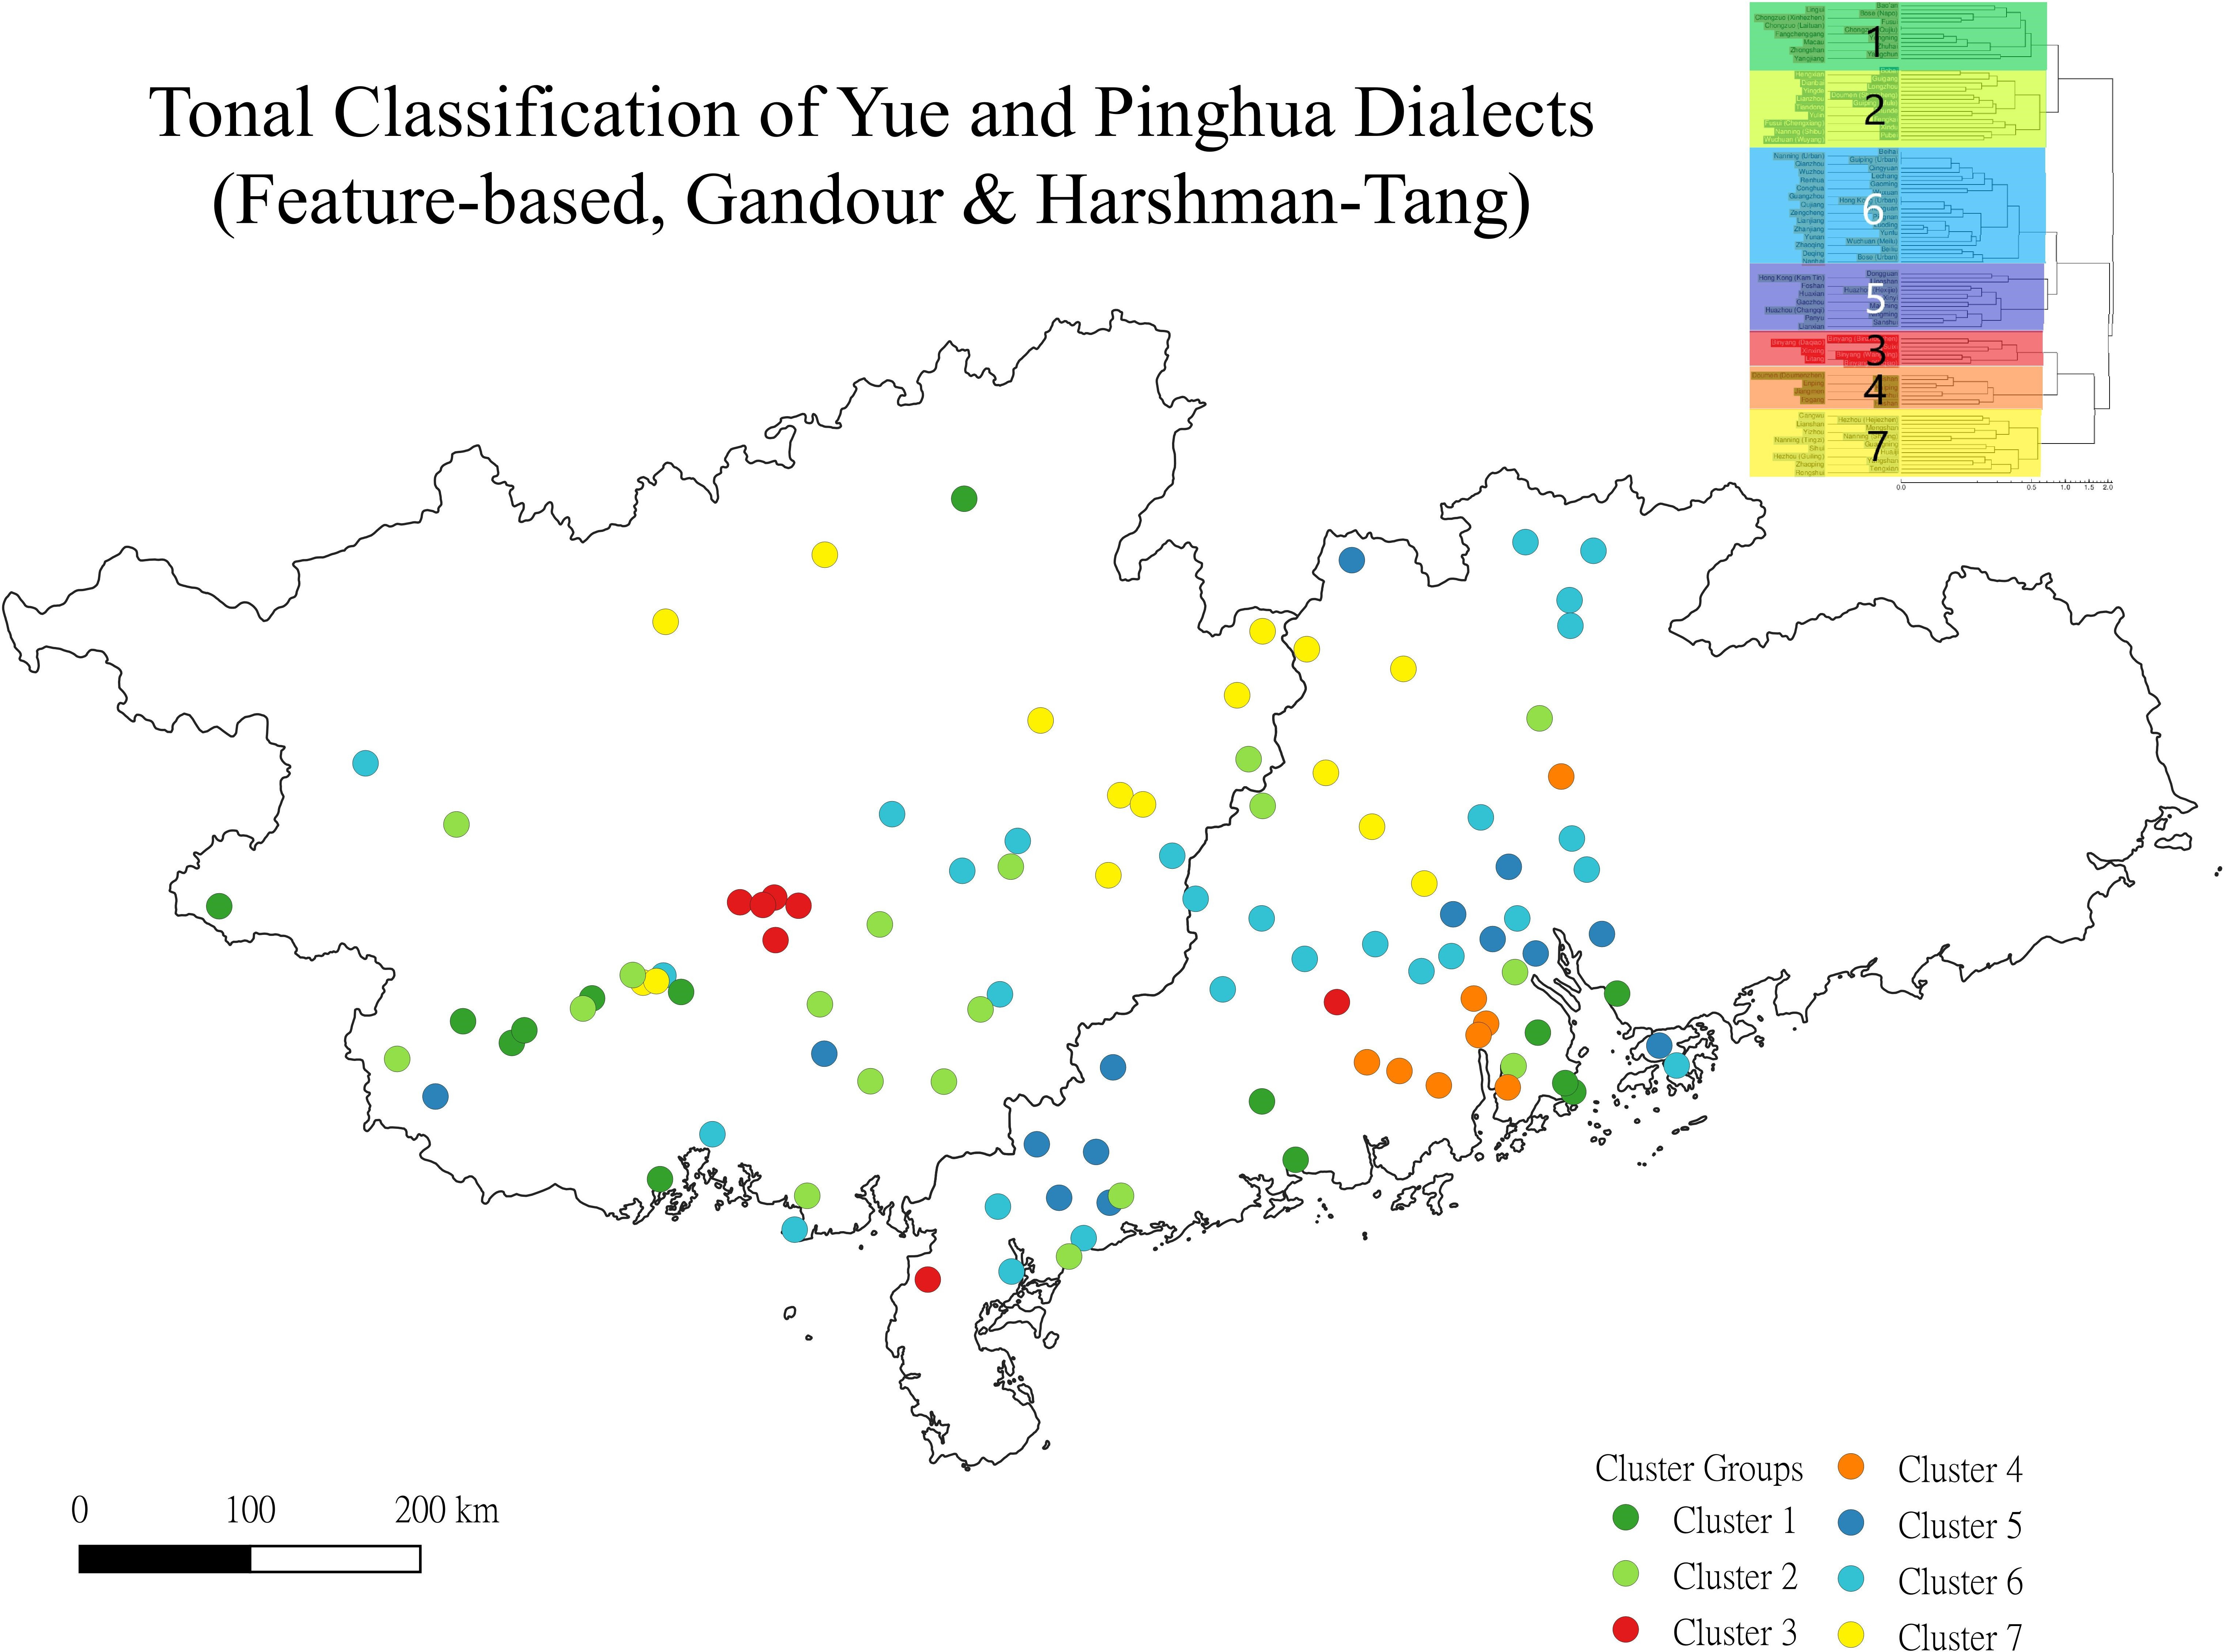
\includegraphics[width=16cm]{sung-map006_2.jpeg}
\caption{\label{map:sung:6} Cluster map (Ward’s method) of the tonal classification of the Yue-Pinghua data (GH-T)}
\end{sidewaysfigure}


\printbibliography[heading=subbibliography,notkeyword=this]


\end{document}
